%- - - - - - - - - - - - - - - - - - - - - - - - - - - - - - - - - - - -
%- - - - - - - - - - - - - - - - - - - - - - - - - - - - - - - - - - - -
%  QPLIB.tex
%- - - - - - - - - - - - - - - - - - - - - - - - - - - - - - - - - - - -
%- - - - - - - - - - - - - - - - - - - - - - - - - - - - - - - - - - - -

\newif\ifMPC
\global\MPCtrue

%- - - - - - - - - - - - - - - - - - - - - - - - - - - - - - - - - - - -

\ifMPC
 \documentclass[smallextended]{svjour3}
 \smartqed
 \journalname{Mathematical Programming Computation}
\else
 \documentclass[12pt,A4wide]{article}
\fi

\usepackage{url}
\usepackage{secdot}
\usepackage{color}
\usepackage{booktabs}
\usepackage{amsmath,amsfonts,amssymb}
\usepackage{amssymb}
\usepackage{amsmath}
\usepackage{multirow}
\usepackage{todonotes}

\usepackage{longtable}
\usepackage{enumitem}
\usepackage{calc}

%- - - - - - - - - - - - - - - - - - - - - - - - - - - - - - - - - - - -
% page size

\ifMPC
\else
 \setlength{\textwidth}{16 cm}
 \setlength{\topmargin}{0 cm}
 \setlength{\headsep}{0 cm}
 \setlength{\textheight}{24 cm}
 \setlength{\evensidemargin}{0cm}
 \setlength{\oddsidemargin}{0cm}
\fi

%- - - - - - - - - - - - - - - - - - - - - - - - - - - - - - - - - - - -
%- - - - - - - - - - - - - - - - - - - - - - - - - - - - - - - - - - - -

\def\NN{\mathbb{N}}
\def\RR{\mathbb{R}}
\def\Mcq{\mathcal{Q}}
\def\Mcl{\mathcal{L}}
\def\Mcm{\mathcal{M}}
\def\Mcn{\mathcal{N}}
\def\Mcb{\mathcal{B}}
\def\Mcr{\mathcal{R}}
\def\Mcu{\mathcal{U}}
\def\Mcx{\mathcal{X}}
\def\Mcz{\mathcal{Z}}

%- - - - - - - - - - - - - - - - - - - - - - - - - - - - - - - - - - - -
% Theorem-like environment definitions

\ifMPC
\else
\newtheorem{theorem}{Theorem}
\newtheorem{assumption}[theorem]{Assumption}
\newtheorem{corollary}[theorem]{Corollary}
\newtheorem{definition}[theorem]{Definition}
\newtheorem{lemma}[theorem]{Lemma}
\newtheorem{remark}{Remark}

\newenvironment{example}{\begin{EX}\rm}{\end{EX}}

\newenvironment{proof}[1][Proof]{\textbf{#1.} }{\ \rule{0.5em}{0.5em}}
%\renewenvironment{proof}{{\bfseries Proof}}{\qed}

\def\remark{\stepcounter{theorem}\par{\bf Remark}.
\ignorespaces}
\def\endremark{ \vbox{\hrule\hbox{%
    \vrule height1.3ex\hskip0.8ex\vrule}\hrule
   }\par}

\newenvironment{keywords}{\vspace{0.4in}\begin{quote}\small \em
{\bf Keywords\/}:}{\end{quote}}
\fi

%- - - - - - - - - - - - - - - - - - - - - - - - - - - - - - - - - - - -
%- - - - - - - - - - - - - - - - - - - - - - - - - - - - - - - - - - - -

\begin{document}

%- - - - - - - - - - - - - - - - - - - - - - - - - - - - - - - - - - - -
%- - - - - - - - - - - - - - - - - - - - - - - - - - - - - - - - - - - -

\title{QPLIB: A Library of Quadratic Programming Instances}

\ifMPC
\titlerunning{QPLIB}
\fi

%- - - - - - - - - - - - - - - - - - - - - - - - - - - - - - - - - - - -
%- - - - - - - - - - - - - - - - - - - - - - - - - - - - - - - - - - - -

\ifMPC
\author{Fabio Furini \and
        Emiliano Traversi \and
        Pietro Belotti \and
        Antonio Frangioni \and
        Ambros Gleixner \and
        Nick Gould \and
        Leo Liberti \and
        Andrea Lodi \and
        Ruth Misener \and
        Hans Mittelmann \and
        Nick Sahinidis \and
        Stefan Vigerske \and
        Angelika Wiegele
        }

\institute{Fabio Furini \at
           LAMSADE, Universit{\'e} Paris Dauphine, 75775 Paris, France.
           \email{fabio.furini@dauphine.fr}
%
\and
           Emiliano Traversi \at
           LIPN, Universit{\'e} de Paris 13, 93430 Villetaneuse, France.
           \email{emiliano.traversi@lipn.fr}
%
\and       Pietro Belotti \at
           Xpress-Optimizer team, FICO, Birmingham UK
           \email{pietrobelotti@fico.com}
%
\and       Antonio Frangioni \at
           Dipartimento di Informatica, Universit\`a di Pisa,
           Largo B. Pontecorvo 2, 56127 Pisa, Italy,
           \email{frangio@di.unipi.it}
%
\and       Ambros Gleixner \at
           Zuse Institute Berlin, Takustr. 7, 14195 Berlin, Germany.
           \email{gleixner@zib.de}
%
\and       Nick Gould \at
           STFC-Rutherford Appleton Laboratory, Chilton, Oxfordshire OX11 0QX,
           England.
           \email{nick.gould@stfc.ac.uk}
%
\and       Leo Liberti \at
           CNRS LIX, Ecole Polytechnique, 91128 Palaiseau, France.
           \email{liberti@lix.polytechnique.fr}
%
\and       Andrea Lodi \at
           Ecole Polytechnique de Montréal, Canada.               \email{andrea.lodi@polymtl.ca}
%
\and       Ruth Misener \at
           Department of Computing,Imperial College London, UK. \email{r.misener@imperial.ac.uk}
%
\and       Hans Mittelmann \at
           School of Mathematical and Statistical Sciences, Arizona State University,      Tempe, AZ 85287-1804, U.S.A.
\email{mittelmann@asu.edu}
%
\and       Nick Sahinidis \at
Chemical Engineering, Carnegie Mellon University, U.S.A. \email{sahinidis@cmu.edu}
%
\and       Stefan Vigerske \at
           GAMS Software GmbH, c/o Zuse Institute Berlin, Takustr. 7, 14195 Berlin, Germany.
           \email{svigerske@gams.com}
%
\and       Angelika Wiegele \at
Institut f{\"u}r Mathematik, Alpen-Adria-Universit{\"a}t Klagenfurt, 9020 Klagenfurt am W{\"o}rthersee, Austria.  \email{angelika.wiegele@aau.at}
           }

\else

\author{Fabio Furini\\
%
\and
        Emiliano Traversi\\
%
\and    Pietro Belotti\\
%
\and    Antonio Frangioni\\
%
\and    Ambros Gleixner\\
%
\and    Nick Gould\\
%
\and    Leo Liberti\\
%
\and    Andrea Lodi\\
%
\and    Ruth Misener\\
%
\and    Hans Mittelmann\\
%
\and    Nick Sahinidis\\
%
\and    Stefan Vigerske\\
%
\and    Angelika Wiegele
        }
\fi

%- - - - - - - - - - - - - - - - - - - - - - - - - - - - - - - - - - - -
%- - - - - - - - - - - - - - - - - - - - - - - - - - - - - - - - - - - -

\ifMPC
 \date{Received: date / Accepted: date}
\else
 \date{}
\fi

\maketitle

\begin{abstract}
 This paper describes a new instance library for Quadratic Programming (QP).\todo[inline]{As we don't use the usual definition of QP, we should already say in the abstract what we understand under a QP.}
 QP is a very ``varied'' class, comprising sub-classes of problems ranging from
 trivial to undecidable. Solution methods for QP are very diverse, ranging from
 entirely combinatorial ones to completely continuous ones, including many for
 which both aspects are fundamental. Selecting a set of instances of QP that is
 at the same time not overwhelmingly numerous and sufficiently challenging for the
 many different interested communities is therefore important. We propose a simple
 taxonomy for QP instances that leads to a systematic problem selection mechanism.
 We then briefly survey the field of QP, giving an overview of theory, methods and
 solvers. Finally we describe how the library was put together, and detail its final
 contents.
\end{abstract}

\ifMPC
 \keywords{Instance Library, Quadratic Programming}

 \subclass{90C06 \and 90C25}
\else
 \begin{keywords}
  Instance Library, Quadratic Programming
 \end{keywords}
\fi


%- - - - - - - - - - - - - - - - - - - - - - - - - - - - - - - - - - - -

%- - - - - - - - - - - - - - - - - - - - - - - - - - - - - - - - - - - -
%- - - - - - - - - - - - - - - - - - - - - - - - - - - - - - - - - - - -
%  QPLIB-1.0.tex
%- - - - - - - - - - - - - - - - - - - - - - - - - - - - - - - - - - - -
%- - - - - - - - - - - - - - - - - - - - - - - - - - - - - - - - - - - -

%- - - - - - - - - - - - - - - - - - - - - - - - - - - - - - - - - - - -
%- - - - - - - - - - - - - - - - - - - - - - - - - - - - - - - - - - - -
\section{Introduction}\label{sec:intro}

Quadratic Programming (QP) problems, where either the objective function \cite{wiki:qp}, or the constraints \cite{wiki:qcqp}, or both contain (at most) expressions in the variables of degree $2$, include a surprisingly diverse set of rather different instances. This is not surprising, given the vast scope of practical applications of these problems, and of solution methods designed to solve them \cite{GoulToin00a}. According to the fine details of the formulation, solving a QP may require employing either fundamentally combinatorial techniques, or ideas rooted in nonlinear optimization principles, or a mix of the two. In this sense, QP is likely one of the classes of problems where the collaboration between the communities interested in combinatorial and nonlinear optimization is more necessary, and potentially fruitful.

However, this diversity also implies that QP means very different things to different researchers. This is illustrated by the simple fact that the class of problems that we simply refer to here as ``QP'' is called in different ways, among which Mixed-Integer Quadratically Constrained Quadratic Problems (MI-QCQP). It is perhaps therefore not surprising that, unlike for ``simpler'' problems classes \cite{Koch2011}, so far there has never been a single library containing all different kinds of instances of QP. Several libraries devoted to special cases of QP are indeed available; however, each of them is either focussed on one application (a specific problem that can be modeled as QP), or on QPs with specific structural properties that make them suitable to be solved with some given class of algorithmic approaches. To the best of our knowledge, collecting a set of QP instances that is at the same time not overwhelmingly numerous and significant for the many different interested communities has not been attempted, yet. This work constitutes a first step in this direction.

In this paper we report the steps that have been done to collect a (hopefully) significant library of QP instances, filtering the large set of available (or specifically provided) instances in order to end up with a manageable set that still contains a meaningful sample of all possible QP types. A particularly thorny issue in this process is how to select instances that are ``interesting''. Our choice has been to take this to mean ``challenging for a significant set of solution methods''. Our filtering process has then been in part based on the idea that if a significant fraction of the solvers that can solve a QP instance do so in a ``short'' time, then the instance is not challenging enough to be included in the library. Yet, if very few (maybe one) solvers can solve it very efficiently by exploiting some specific structure, but most other approaches cannot, then the instance can still be deemed ``interesting''. Putting this approach in practice requires a nontrivial number of technical steps and decisions that are detailed in the paper. We hope that our work can provide useful guidelines for other interested researchers.

A consequence of our focus is that this paper is \emph{not} concerned about the different performance of the very diverse QP solvers; we will \emph{not} report any data comparing them. The only reason why solvers are used (and, therefore, described) in this context is to ensure that the instances of the library are nontrivial at least for a significant fraction of the current solution methods; providing guidance about which solver is most suited to some specific class of QPs is entirely outside the scope of our work.

%- - - - - - - - - - - - - - - - - - - - - - - - - - - - - - - - - - - -
\subsection{Motivation}\label{subsec:motiv}

Optimization problems with quadratic constraints and/or objective function (QP) have been the subject of a considerable amount of research over the last 60 years. At least some of the rationale for this interest is likely due to the fact that they are the ``least-nonlinear nonlinear problems''. Hence, in particular for the convex case, tools and techniques that have been honed during decades of research for Linear Programming (LP), typically with integrality constraints (MILP), can often be extended to the quadratic case with at least less effort than what would be required for tackling general Non Linear Programming (NLP) problems, without or with integrality constraints (MINLP). This has indeed happened over and over again with different algorithmic techniques, such as Interior Point methods, active-set methods (of which the simplex method is a prototypical example), enumeration methods, cut-generation techniques, reformulation techniques, and many others \cite{BS09}.
Similarly, nonconvex continuous QP are perhaps the ``simplest'' class of problems that require features like spatial enumeration techniques to be solved.
Hence, they are both the natural basis for the development of general techniques for nonconvex NLP, and a very specific class so that specialized approaches can be developed \cite{Dur2010,Burer2012}.

On the other hand, (MI)QP is, in some sense, a considerably more expressive class than (MI)LP. Quadratic expressions are found, either naturally or after appropriate reformulations, in very many optimization problems \cite{Kochenberger2014}. Table \ref{tbl:application} provides a certainly non-exhaustive collection of applications that lead to formulations with either quadratic constraints, or quadratic objective function, or both. Also, in general any continuous function can be approximated with arbitrary accuracy (over a compact set) by a polynomial of arbitrary degree; in turn, every polynomial can be broken down to a system of quadratic expressions. Hence, (MI)QP is, in some sense, roughly as expressive as the whole of (MI)NLP. Of course this is, in principle, true for (MI)LP as well, but at the cost of much larger and much more complex formulations. Hence, for many applications QP may represent the ``sweet spot'' between the effectiveness, but lower expressive power, of (MI)LP and the higher expressive power, but much higher computational cost, of (MI)NLP.


\begin{longtable}[c]{lcl}
%
\caption{Application Domains of (MI)QP}\label{tbl:application} \\
%
\toprule
Problem & Discrete & Contributions \\
\midrule
\endfirsthead
%
\multicolumn{3}{l}{\emph{Table \ref{tbl:application} (Application Domains of (MI)QP) continued}} \\
\toprule
Problem & Discrete & Contributions \\
\midrule
\endhead
%
\midrule
\multicolumn{3}{l}{\multirow{1}{.95\textwidth}{$^{\ddagger}$Applications with many manuscripts cite reviews and recent works \\[-12pt] \phantom{hi}  \hfill\emph{continued}}}
\endfoot
%
\bottomrule
\multicolumn{3}{l}{\multirow{1}{.95\textwidth}{$^{\ddagger}$Applications with many manuscripts cite reviews and recent works.}}
\endlastfoot
%
\multicolumn{3}{l}{\textbf{Classical Problems that can be formulated as MIQP}} \\[1pt]
%
Quadratic Assignment Problem$^{\ddagger}$ & \checkmark & \cite{anstreicher:2003,loiola-etal:2007} \\ \cmidrule(rl){2-3}
%
Max-Cut & \checkmark & \cite{Rendl2008,KrislockMalickRoupin2016} \\ \cmidrule(rl){2-3}
%
Maximum clique$^{\ddagger}$ & \checkmark & \cite{bomze-etal:1999} \\
\midrule
%
\multicolumn{3}{l}{\textbf{Computational chemistry \& Molecular biology}} \\[1pt]
%
Zeolites && \cite{gounaris-etal:2013} \\
\midrule
%
\multicolumn{3}{l}{\textbf{Computational geometry}} \\[1pt]
%
Layout design & \checkmark & \cite{anjos-liers:2012,castillo-etal:2005,dorneich-sahinidis:1995} \\ \cmidrule(rl){2-3}
%
Maximizing polygon dimensions && \cite{audet-etal:2011,audet-etal:2007,Audet-etal:2009,audet-etal:2002,Audet-Ninin:2013} \\ \cmidrule(rl){2-3}
%
Packing circles$^{\ddagger}$ & \checkmark & \cite{FrFG16,FGGP11,hifi-mhallah:2009,szabo-etal:2005} \\ \cmidrule(rl){2-3}
%
Nesting polygons && \cite{kallrath:2009,rebennack-etal:2009} \\ \cmidrule(rl){2-3}
%
Cutting ellipses && \cite{kallrath-rebennack:2013} \\ %\cmidrule(rl){2-3}
%Nonconvex shapes \\
\midrule
%
\multicolumn{3}{l}{\textbf{Finance}} \\[1pt]
Portfolio optimization & \checkmark & \multirow{1}{.3\textwidth}{\cite{deng-etal:2013,kallrath:2003,lin-etal:2005,maranas-etal:1997,parpas-rustem:2006,rios-sahinidis:2010,FrFG16,FrGe06a,FrGe07a,FrGe09a}} \\ \\
%
\midrule
%
\multicolumn{3}{l}{\textbf{Process Networks}} \\[1pt]
%
%\multicolumn{3}{l}{Process networks optimisation problems typically involve two} \\
%
Crude oil scheduling & \checkmark & \cite{li-etal:2007,li-etal:2011,li-etal:2012,mouret-etal:2009,mouret-etal:2011} \\ \cmidrule(rl){2-3}
%
Data reconciliation & \checkmark & \cite{ruiz-grossmann:2011} \\ \cmidrule(rl){2-3}
%
Multi-commodity flow & \checkmark & \cite{tadayon-smith:2013} \\ \cmidrule(rl){2-3}
%
Quadratic network design & \checkmark & \cite{FrFG16,FGGP11} \\ \cmidrule(rl){2-3}
%
Multi-period blending & \checkmark & \cite{kolodziej-etal:2013:jogo,kolodziej-etal:2013} \\ \cmidrule(rl){2-3}
%
Natural gas networks & \checkmark & \cite{hasan-etal:2011,li-etal:2011-aiche_journal,li-etal:2011-jogo} \\ \cmidrule(rl){2-3}
%
Pooling$^{\ddagger}$ & \checkmark & \multirow{1}{.3\textwidth}{\cite{Alfaki-Haugland:2013,Castillo-etal:2013,dambrosio-etal:2011pooling,Faria-Bagajewicz:2012,misener-floudas:2009,misener-floudas:2010-genpooling,Papageorgiou-etal:2012,pham-etal:2009,ruiz-etal:2013}} \\ \\ \cmidrule(rl){2-3}
%
Open-pit mine scheduling & \checkmark & \cite{bley-etal:2012} \\ \cmidrule(rl){2-3}
%
Reverse osmosis & \checkmark & \cite{saif-etal:2008} \\ \cmidrule(rl){2-3}
%
Supply chain & \checkmark & \cite{nyberg-etal:2012} \\ \cmidrule(rl){2-3}
%
Water networks$^{\ddagger}$ & \checkmark & \multirow{1}{.3\textwidth}{\cite{ahmetovic-grossmann:2010,bagajewicz:2000,bragalli-etal:2011,castro-teles:2013,geissler-etal:2013,gleixner-etal:2012,jezowski-2010,khor-etal:2014,ponceortega-etal:2010,teles-etal:2012}} \\ \\
%
\midrule
%
\multicolumn{3}{l}{\textbf{Robotics}} \\[1pt]
%
Traveling Salesman Problem \\
with Neighborhoods & \checkmark & \cite{gentilini-etal:2013} \\
\midrule
%
\multicolumn{3}{l}{\textbf{Telecommunications}} \\[1pt]
%
Delay-constrained routing & \checkmark & \cite{FrGaSc14,FrGaSt16a} \\
\midrule
%
\multicolumn{3}{l}{\textbf{Energy}} \\[1pt]
%
Unit-commitment & \checkmark & \cite{FrFG16,FrGe06a,FrGe09a,Tetal15} \\
\midrule
%
\multicolumn{3}{l}{\textbf{Data Confidentiality}} \\[1pt]
%
Controlled Tabular Adjustment & \checkmark & \cite{CaFG14}
\end{longtable}



The structure of this paper is the following. In \S\ref{sec:QPbasic} we review the basic notion of QP. In particular, \S\ref{subsec:notation} sets out the notation, \S\ref{sec:classification} proposes a---to the best of our knowledge, new---taxonomy of QP that helps us in discussing the (very) different classes of QPs, \S\ref{sec:algo} very briefly reviews the solution methods for QP and the solvers we have employed.
Then, \S\ref{sec:lib} describes the process used to obtain the library and its results.
%; the software tools that we have used, and that are freely released together with the library, are discussed in \S\ref{subsec:tools}.
Some conclusions are drawn in \S\ref{sec:conclusions}, after which Appendix A provides a complete description of all the instances of the library, while Appendix B describes the QPLIB file format.


While no performance issues of solvers for QP/QCP problems are considered in
this paper, we refer to the comprehensive benchmark site \url{http://plato.asu.edu/bench.html}. Of the benchmarks
on this site three deal exlusively with QP/QCP problems:
the (1) Large SOCP, (2) MISOCP, and the (3) MIQ(C)P benchmarks.
The following contain partly results for such problems:
(4) Parallel Barrier Solvers on Large LP/QP problems, (5) AMPL-NLP, (6) MINLP.
The benchmarks (1,2,4) have only convex instances, while the others include
nonconvex instances. Global optima are obtained by several of the solvers in
the benchmarks (3,5).
All solvers in the latest addition (6) compute global optima, they are ANTIGONE,
BARON, COUENNE, LINDO, and SCIP, c.f.~\S\ref{subsec:solver}. This benchmark is based on MINLPLib~2 \cite{Vigerske2014}, a
collection of presently 1388 instances. In order to give a first representative
impression of solver performance, care was taken to reduce the number of instances and
allow all solvers to finish in reasonable time. More than half of the selected
instances are QP or QCP. A time limit of two hours on a
modern workstation with sufficient memory was used. Computations were done in
GAMS with scripts derived from the SCIP check scripts and available at GitHub.
For details we refer to \url{http://plato.asu.edu/ftp/minlp.html}.

%- - - - - - - - - - - - - - - - - - - - - - - - - - - - - - - - - - - -
%- - - - - - - - - - - - - - - - - - - - - - - - - - - - - - - - - - - -
%  End QPLIB-1.0.tex
%- - - - - - - - - - - - - - - - - - - - - - - - - - - - - - - - - - - -
%- - - - - - - - - - - - - - - - - - - - - - - - - - - - - - - - - - - -


%- - - - - - - - - - - - - - - - - - - - - - - - - - - - - - - - - - - -

%- - - - - - - - - - - - - - - - - - - - - - - - - - - - - - - - - - - -

%- - - - - - - - - - - - - - - - - - - - - - - - - - - - - - - - - - - -
%- - - - - - - - - - - - - - - - - - - - - - - - - - - - - - - - - - - -
%  QPLIB-2.1.tex
%- - - - - - - - - - - - - - - - - - - - - - - - - - - - - - - - - - - -
%- - - - - - - - - - - - - - - - - - - - - - - - - - - - - - - - - - - -

%- - - - - - - - - - - - - - - - - - - - - - - - - - - - - - - - - - - -
%- - - - - - - - - - - - - - - - - - - - - - - - - - - - - - - - - - - -
\section{Quadratic Programming in a nutshell}\label{sec:QPbasic}

%- - - - - - - - - - - - - - - - - - - - - - - - - - - - - - - - - - - -
\subsection{Notation}\label{subsec:notation}

In mathematical optimization, a Quadratic Program (QP) is an optimization problem in which either the objective function, or some of the constraints, or both, are quadratic functions. More specifically, the problem has the form
%
\begin{align*}
 \min \textrm{or} \max \;\;
 & {\textstyle \half} x^\top Q^0 x + b^0 x + q^0 \\
 \textrm{such that}\;\;
 & c^i_l \leq {\textstyle \half} x^\top Q^i x + b^i x \leq c^i_u & i \in \Mcm, \\
 %
 & l_j \leq x_j \leq u_j & j \in \Mcn,  \\
 %
 \textrm{and}\;\;
 & x_j \in \mathbb{Z} & j \in \Mcz,
\end{align*}
%
%\begin{align*}
% \min \;\;
% & x^\top Q^0 x + b^0 x \\
% %
% & x^\top Q^i x + b^i x \leq c^i & i \in \Mcm \\
% %
% & l_j \leq x_j \leq u_j & j \in \Mcn  \\
% %
% & x_j \in \mathbb{Z} & j \in \Mcz
%\end{align*}
%
where
%
\begin{itemize}
 \item $\Mcn = \{ 1, \ldots, n \}$ is the set of (indices) of variables, and $\Mcm = \{ 1, \ldots, m \}$ is the set of (indices) of constraints;
 %
 \item $x = [x_j]_{j = 1}^n$ %\in \RR^n$
is a finite vector of real variables;
 %
 \item $Q^i$ for $i \in \{ 0 \} \cup \Mcm$ are symmetric $n \times n$ real (Hessian) matrices: since one is only interested in the value of quadratic forms of the type $x^\top Q^i x$, symmetry can be assumed without loss of generality by just replacing off diagonal pairs $Q^i_{hk}$ and $Q^i_{kh}$ with their average $(Q^i_{hk} + Q^i_{kh}) / 2$;
 %
 \item $b^i$, $c_u^i$, $c_l^i$ for $i \in \{ 0 \} \cup \Mcm$, and $q^0$ are, respectively, real $n$-vectors and real constants;
 %
 \item $-\infty \leq l_j \leq u_j \leq \infty$ are the (extended) real lower and upper bounds on each variable $x_j$ for $j \in \Mcn$;
 %
 \item $\Mcm = \Mcq \cup \Mcl$ where $Q^i = 0$ for all $i \in \Mcl$ (i.e., these are the linear constraints, as opposed to the truly quadratic ones); and
 %
 \item the variables in $\Mcz \subseteq \Mcm$ are restricted to only attain integer values.
\end{itemize}
%
Due to the presence of integrality requirements on the variables and of quadratic constraints, this class of problems is often referred to as Mixed-Integer Quadratically Constraint Quadratic Program (MIQCQP). It will be sometimes useful to refer to the (sub)set $\Mcb =  \{ \, j \in \Mcz : l_j = 0 , u_j = 1 \, \} \subseteq \Mcz$ of the binary variables, and to $\Mcr = \Mcn \setminus \Mcz$ as the set of continuous ones. Similarly, it will be sometimes useful to distinguish the (sub)set $\Mcx = \{ \, j : l_j > -\infty \lor u_j < \infty \, \}$ of the box-constrained variables from $\Mcu = \Mcn \setminus \Mcx$ of the unconstrained ones (in the sense that finite bounds are not explicitly provided in the data of the problem, although they may be implied by the other constraints).

The relative flexibility offered by quadratic functions, as opposed e.g.~to linear ones, allows several reformulation techniques to be applicable to this family of problems in order to emphasize different properties of the various components. Some of these reformulation techniques will be commented later on; here we remark that, for instance, integrality requirements, in particular in the form of binary variables could always be ``hidden'' by introducing (nonconvex) quadratic constraints utilizing the celebrated relationship $x_j \in \{0, 1\} \iff x_j^2 = x_j$. Therefore, when discussing these problems some effort has to be made to distinguish between features that come from the original model, and those that can be introduced by reformulation techniques in order to extract (and algorithmically exploit) specific properties.

\textcolor{red}{In the rest of this paper, we shall sometimes refer to {\it exact solutions} of quadratic programs. In view of the fact that their solutions may be irrational, this notation deserves a comment. If the decision version of the problem being referred to is in NP (e.g.~LP, MILP, QP \cite{vavasis90a}), then the assumption is that all rational numbers can be represented exactly by a Turing Machine (TM). 
%This assumption has the same limitation as the assumption that TMs defined on integers are a faithful abstraction of a real computer, namely that the range of integers needing a representation is bounded. 
If there is no known proof that the problem being solved (or its decision version) is in NP, then there are four main approaches:
\begin{enumerate}
\item finding a representable solution $x'$ such that $\|x'-x^\ast\|_\infty\le\varepsilon$, where $x^\ast$ is the true solution, $\varepsilon>0$ is given, and representable means having a polynomially sized description length
% ``
(in function of the instance size) \cite{hochbaum2};
\item using the {\it Thom encoding} of an algebraic number \cite[Prop.~2.28]{pollack} (limited to problems involving polynomials);
\item using the optimality gap: finding a representable solution $x'$ such that $|f(x')-f(x^\ast)|\le\varepsilon$, where $f$ is the objective function, $x^\ast$ is the true solution, $\varepsilon>0$ is given
%, and representable is as above 
(limited to optimization problems);\label{optgap}
\item using a computational model according to which every elementary computation on the reals takes $O(1)$ and returns an exact result \cite[p.~24]{blum}.
\end{enumerate}
Approach \ref{optgap} in the list above is the one most often used in computational papers, including the present one.}


%- - - - - - - - - - - - - - - - - - - - - - - - - - - - - - - - - - - -
%- - - - - - - - - - - - - - - - - - - - - - - - - - - - - - - - - - - -
%  End QPLIB-2.1.tex
%- - - - - - - - - - - - - - - - - - - - - - - - - - - - - - - - - - - -
%- - - - - - - - - - - - - - - - - - - - - - - - - - - - - - - - - - - -


%- - - - - - - - - - - - - - - - - - - - - - - - - - - - - - - - - - - -

%- - - - - - - - - - - - - - - - - - - - - - - - - - - - - - - - - - - -

%- - - - - - - - - - - - - - - - - - - - - - - - - - - - - - - - - - - -
%- - - - - - - - - - - - - - - - - - - - - - - - - - - - - - - - - - - -
%  QPLIB-2.2.tex
%- - - - - - - - - - - - - - - - - - - - - - - - - - - - - - - - - - - -
%- - - - - - - - - - - - - - - - - - - - - - - - - - - - - - - - -


%- - - - - - - - - - - - - - - - - - - - - - - - - - - - - - - - - - - -
\subsection{Classification}\label{sec:classification}

Despite the apparent simplicity of the definition given in \S\ref{subsec:notation}, Quadratic Programming instances can be of several rather different ``types'' in practice, depending on fine details of the data. In particular, many algorithmic approaches can only be applied to QP when the data of the problem has specific properties. A taxonomy of QP instances should thus strive to identify the set of properties that an instance should have in order to apply the most relevant computational methods. However, the sheer number of different existing approaches, and the fact that new ones are frequently proposed, makes it hard to provide a taxonomy that is both simple and covers all possible special cases. This is why, in this paper, we propose an approach that aims at finding a good balance between simplicity and coverage of the main families of computational methods.

% -  -  -  -  -  -  -  -  -  -  -  -  -  -  -  -  -  -  -  -  -  -  -  -
\subsubsection{Taxonomy}\label{ssec:taxonomy}


Our taxonomy is based on a three-fields code of the form ``\textit{OVC}'', where \textit{O} indicates the type of objective function considered, \textit{V} records the types of variables, and \textit{C} designates the types of constraints imposed on the variables. The fields can be given the following values:
%
\begin{itemize}
 \item objective function: (\textit{L})inear, (\textit{D})iagonal convex (if minimization) or concave (if maximization) quadratic, (\textit{C})onvex (if minimization) or (\textit{C})oncave (if maximization) quadratic,  (\textit{Q})uadratic (all other cases);
 %
 \item variables: (\textit{C})ontinuous only, (\textit{B})inary only, (\textit{M})ixed binary and continuous, (\textit{I})nteger (including binary) only, (\textit{G})eneral (all other cases);
 %
 \item constraints: (\textit{N})one, (\textit{B})ox, (\textit{L})inear, (\textit{D})iagonal convex quadratic, (\textit{C})onvex quadratic, nonconvex (\textit{Q})uadratic.
\end{itemize}
%
The wildcard ``*'' will be used below to indicate any possible choice, and lists of the form ``\{\textit{X}, \textit{Y}, \textit{Z}\}'' will indicate that the value of the given field can freely attain any of the specified values.

The ordering of the values in the previous lists is not irrelevant; in general, problems become ``harder'' when going from left to right. More specifically, for the \textit{O} and \textit{C} fields the order is that of \emph{strict} containment between problem classes: for instance, linear objective functions are strictly a special case of diagonal convex quadratic ones (by allowing the diagonal elements all to be zero), the latter are a strict subset of general convex quadratic objectives (by allowing the off-diagonal elements all to be zero), and these are strictly subsets of general nonconvex quadratic ones (since these permit any symmetric Hessian including positive semidefinite ones). The only field for which the containment relationship is not a total order is \textit{V}, for which only the partial orderings
\[
 \mbox{\textit{C}} \subset \mbox{\textit{M}} \subset \mbox{\textit{G}},
 \qquad
 \mbox{\textit{B}} \subset \mbox{\textit{M}} \subset \mbox{\textit{G}},
 \qquad
 \mbox{and}
 \qquad
 \mbox{\textit{B}} \subset \mbox{\textit{I}} \subset \mbox{\textit{G}}
\]
hold. In the following discussion we will repeatedly exploit this by assuming that, unless otherwise mentioned, when a method can be applied to a given problem, it can be applied as well to all simpler problems where the value of each field is arbitrarily replaced with a value denoting a less-general class.

% -  -  -  -  -  -  -  -  -  -  -  -  -  -  -  -  -  -  -  -  -  -  -  -
\subsubsection{Examples and reformulations}\label{ssec:reform}

We now give a general discussion about the different problem classes that our proposed taxonomy defines.
For simplicity, we will assume minimization problems for the remaining of this section.
Some problem classes are actually ``too simple'' to make sense in our context. For instance, D*B problems have only diagonal quadratic (hence separable) objective function and bound constraints; as such, they read
\[
 \textstyle
 \min \; \Big\{ \,
 \sum_{j \in \Mcn} \big( \, \half Q^0_j x_j^2 + b^0_j x_j \, \big) \;:\;
 l_j \leq x_j \leq u_j \quad j \in \Mcn \;\;,\;\;
 x_j \in \mathbb{Z} \quad j \in \Mcz \, \Big\}
 \;\; .
\]
Hence, their solution only requires the independent minimization of a convex quadratic univariate function in each single variable $x_j$ over a box constraint and possibly integrality requirements, which can be attained trivially in $O(1)$ operations (per variable) by closed-form formul{\ae}, projection and rounding arguments. \emph{A fortiori}, the even simpler cases \textit{L*B}, \textit{D*N} and \textit{L*N} (the latter obviously unbounded unless $b^0 = 0$) will not be discussed here. Similarly, \textit{CCN} are immediately solved by linear algebra techniques, and therefore are of no interest in this context. At the other end of the spectrum, in general QP is a hard problem. Actually, \textit{LIQ}---linear objective function and quadratic constraints in integer variables with no finite bounds, i.e.
\[
 \textstyle
 \min \; \Big\{ \, b^0 x \;:\;
 \half x^\top Q^i x + b^i x \leq c^i \quad i \in \Mcm \;\;,\;\;
 x_j \in \mathbb{Z} \quad j \in \Mcn \, \Big\}
 \;\; ,
\]
is not only $\mathcal{NP}$-hard, but downright undecidable \cite{jeroslow}. Hence so are the ``harder'' \{\textit{C},\textit{Q}\}\textit{IQ}.

\smallskip
It is important to note that the relationships between the different classes can be somehow blurred because reformulation techniques may allow one to move an instance from one class to another. We already mentioned that $x^2 = x \iff x \in \{0, 1\}$, and in general \textit{*M*}---instances with only binary and continuous variables---can be recast as \textit{*CQ}; here nonconvex quadratic constraints take the place of binary variables. More generally, this is also true for \textit{*G*} as long as $\Mcu = \emptyset$, as bounded general integer variables can be represented by binary ones.

Another relevant reformulation trick concerns the fact that, as soon as quadratic constraints are allowed, then there is no loss of generality in assuming a linear objective function. Indeed, any \textit{Q**} (\textit{C*C}) problem can always be rewritten as
%
\begin{align*}
 \min \;\;
 & x^0 \\
 %
 & \hspace*{-5mm} -\infty \leq \half x^\top Q^0 x + b^0 x \leq x^0 & \\
 %
 & c^i_l \leq \half x^\top Q^i x + b^i x \leq c^i_u & i \in \Mcm \\
 %
 & l_j \leq x_j \leq u_j & j \in \Mcn  \\
 %
 & x_j \in \mathbb{Z} & j \in \Mcz
\end{align*}
%
i.e., a \textit{L*Q} (\textit{L*C}) pronlem. Hence, it is clear that quadratic constraints are, in a well-defined sense, the most general situation (cf.~also the result above about hardness of \textit{LIQ}).

When a $Q^i$ is positive semidefinite (PSD), i.e., the corresponding constraint/objective function is convex, general Hessians are in fact equivalent to diagonal ones. In particular, since every PSD matrix can be factorized as $Q^i = L^i (L^i)^T$, e.g.~by the (incomplete) Cholesky factorization, the term $\half x^T Q^i x \equiv \half \sum_{j \in \Mcn} z^{i\;2}_j$ where $z^{i\;T} = x^T L^i$. Hence, one might maintain that D** problems need not be distinguished from C** ones. However in reality, this is only true for ``complicated'' constraints but not for ``simple'' ones, because the above reformulation technique introduces additional linear constraints, $L^{i\;T} x - z^i = 0$. Indeed, while \textit{C*L} (and, a fortiori, \textit{C*}\{\textit{C},\textit{Q}\}) can always be brought to \textit{D*L} (\textit{D*}\{\textit{C},\textit{Q}\}), using the above technique \textit{C*B} becomes \textit{D*L}, which may be significantly different from \textit{D*B}. In practice, a diagonal convex objective function under linear constraints is found in many applications (e.g., \cite{FrFG16,FrGe06a,FrGe09a,FGGP11}), so that it still makes sense to distinguish the \textit{D*L} case where the objective function is ``naturally'' separable from that where separability is artificially introduced.

% -  -  -  -  -  -  -  -  -  -  -  -  -  -  -  -  -  -  -  -  -  -  -  -
\subsubsection{QP classes}\label{ssec:classes}

The proposed taxonomy can then be used to describe the main classes of QP according to the type of algorithms that can be applied for their solution:
%
\begin{itemize}
 \item \emph{Linear Programs} \textit{LCL} and \emph{Mixed-Integer Linear Programs} \textit{LGL} have been subject of an enormous amount of research and have their well-established instance libraries \cite{Koch2011}, so they will not be explicitly addressed here.
 %
 \item \emph{Convex Continuous Quadratic Programs} \textit{CCC} can be solved in polynomial time by Interior-Point techniques \cite{Wright97}; the simpler \textit{CCL} can also be solved by means of ``simplex-like'' techniques, usually referred to as active-set methods \cite{Dost09}. Actually, a slightly larger class of problems can be solved with Interior-Point methods: those that can be represented by Second-Order Cone Programs. When written as QPs the corresponding $Q^i$ may not be positive semidefinite, but nonetheless such problems can be efficiently solved. Of course just as for \textit{LCL}, these problems may still require considerable computational effort when the size of the instance grows. In this sense, like in the linear case, there is a significant distinction between solvers that need all the data of QP to work, and those that are ``matrix-free'', i.e., only require the application of simple operations (typically, matrix-vector products) with the problem data. While when building our instance library we never exploited such characteristics, since they are not amenable to standard modelling tools, but this may be relevant for the solution of very-large-scale \textit{CIC}.
 %
 \item \emph{Nonconvex Continuous Quadratic Programs} \textit{QCQ} are generally $\mathcal{NP}$-hard, even if the constraints are very specific (\textit{QCB}) and only a single eigenvalue of $Q^0$ is negative \cite{Hemmecke2010}. They therefore require enumerative techniques, such as spatial Branch\&Bound \cite{FV90,BeLeLiMaWa08}, to be solved to optimality. Of course, local approaches are available that are able to efficiently provide saddle points (hopefully, local optima) of the \textit{CQC}, but providing global guarantees about the quality of the obtained solutions is challenging. In our library we have specifically focused on  \emph{exact} solution of the instances.
  %
 \item \emph{Convex Integer Quadratic Programs} \textit{CGC} are, in general, $\mathcal{NP}$-hard, and therefore require enumerative techniques to be solved. However, convexity of the objective function and constraints implies that efficient techniques (see \textit{CCC}) can be used at least to solve continuous relaxations. The general view is that \textit{CGC} are not, all other things being equal,  substantially more difficult than \textit{LGL} to solve, especially if the objective function and/or the constraints have specific properties (e.g., \textit{DGL}, \textit{CGL}). Often integer variables are in fact binary ones, so several \textit{CCC} models are \textit{C}\{\textit{B},\textit{M}\}\textit{C} ones. In practice binary variables are considered to lead to somewhat easier problems than general integer ones (cf.~the cited result about hardness of unbounded integer quadratic programs), and several algorithmic techniques have been specifically developed for this special case. However, the general approaches for \textit{CBC} are basically the same as for \textit{CGC}, so there is seldom the need to distinguish between the two classes as far as solvability is concerned, although matters can be different regarding actual solution cost. Programs with only binary variables \textit{CBC} can be easier than mixed-binary or integer ones \textit{C}\{\textit{M},\textit{I}\}\textit{C} because some techniques are specifically known for the binary-only case, cf.~the next point \cite{BEP09}. Absence of continuous variables, even in the presence of integer ones \textit{CIC}, can also lead to specific techniques \cite{BEL13}.
  %
  \item \emph{Nonconvex Binary Quadratic Programs} \textit{QB}\{\textit{B}, \textit{N}, \textit{L}\} obviously are $\mathcal{NP}$-hard. However, the special nature of binary variables combined with quadratic forms allows for quite specific techniques to be developed, one of which is the reformulation of the problem as a \textit{LBL}. Also, many well-known combinatorial problems can be naturally reformulated as problems of this class, and therefore a considerable number of results have been obtained by exploiting specific properties of the set of constraints \cite{Rendl2008,Loiola2007657}.
  %
  \item \emph{Nonconvex Integer Quadratic Programs} \textit{QGQ} is the most general, and therefore is the most difficult, class. Due to the lack of convexity even when integrality requirements are removed, solution methods must typically combine several algorithmic ideas, such as enumeration (distinguishing the role of integral variables from that of continuous ones involved into nonconvex terms) and techniques (e.g., outer approximation, semidefinite programming relaxation, \ldots) that allow the efficient computation of bounds. As in the convex case, \textit{QBQ}, \textit{QMQ}, and \textit{QIQ} can benefit from more specific properties of the variables \cite{Buchheim2013,Dong2016}.
\end{itemize}
%
This description is deliberately coarse; each of these classes can be subdivided into several others on the grounds of more detailed information about structures present in their constraints/objective function. These can have a significant algorithmic impact, and therefore can be of interest to researchers. Common structures are, e.g., network flows \cite{FrFG16,FrGaSc14,FrGaSt16a,FGGP11,tadayon-smith:2013} or knapsack-type linear constraints \cite{FrFG16,FrGo13b,FGGP11}, and semi-continuous variables \cite{FrFG16,FrGaSc14,FrGaSt16a,FrGe06a,FrGe07a,FrGe09a,FGGP11}, or the fact that a nonconvex quadratic objective function/constraint can be reformulated as a second-order cone (hence, convex) one \cite{FrFG16,FrGaSc14,FrGaSt16a,FrGe09a,FGGP11}. It would be very hard to collect a comprehensive list of all types of structures that might be of interest to any individual researcher, since these are as varied as the different possible approaches for specialized sub-classes of QP. For this reason we do not attempt such a more refined classification, and limit ourselves to the coarser one described in this section.

%- - - - - - - - - - - - - - - - - - - - - - - - - - - - - - - - - - - -
%- - - - - - - - - - - - - - - - - - - - - - - - - - - - - - - - - - - -
%  End QPLIB-2.2.tex
%- - - - - - - - - - - - - - - - - - - - - - - - - - - - - - - - - - - -
%- - - - - - - - - - - - - - - - - - - - - - - - - - - - - - - - - - - -


%- - - - - - - - - - - - - - - - - - - - - - - - - - - - - - - - - - - -

%- - - - - - - - - - - - - - - - - - - - - - - - - - - - - - - - - - - -

%- - - - - - - - - - - - - - - - - - - - - - - - - - - - - - - - - - - -
%- - - - - - - - - - - - - - - - - - - - - - - - - - - - - - - - - - - -
%  QPLIB-2.3.tex
%- - - - - - - - - - - - - - - - - - - - - - - - - - - - - - - - - - - -
%- - - - - - - - - - - - - - - - - - - - - - - - - - - - - - - - - - - -

\subsection{Solution Methods}\label{sec:algo}

In this section we provide a quick overview of existing solution methods for QP, restricting ourselves to these implemented by the set of solvers considered in this paper (Table \ref{t:solvers}). For each approach we briefly describe the main algorithmic ideas and point out the formulation they address according to the classification set out in Sect.~\ref{sec:classification}. We remark that many solvers implement more than one algorithm, among which the user can choose at runtime. Moreover, algorithms are typically implemented by different solvers in different ways, so that the same conceptual algorithm can sometimes yield wildly different results or performance measures on the same instances.

% antigone/glomiqo: sBB
% baron: sBB
% couenne: sBB
% knitro: IPM with CG, SLQP, convexBB + outerapproxBB
% lindo/lindoglobal: sBB
% scip: sBB
% msnlp/oqnlp: multistart
% alphaecp: cutting plane for pseudoconvex MINLP
% bonmin: convexBB
% dicopt: alternating projection NLP/MILP
% sbb: convexBB
% conopt: GRG (active set -- like SQP)
% ipopt: IPM w/ line search filter
% lgo: Lipschitz BB, random search, multistart (default) [cassato?]
% minos: active set method
% snopt: active set SQP
% xpress: convexBB
% gurobi: convexBB
% cplex: sBB

The methods implemented by the solvers in Table~\ref{t:solvers} can, following \cite{neumaier}, be broadly organized in three categories: {\it incomplete}, {\it asymptotically complete}, and {\it complete}. Incomplete methods are only able to identify solutions, often locally optimal according to a suitable notion, and may even fail to find one even when one exists; in particular, they are typically not able to determine that an instance is empty. Asymptotically complete methods can find a globally optimal solution with probability one in infinite time, but again they cannot prove that a given instance is infeasible. Complete methods find an approximate globally optimal solution to within a prescribed optimality tolerance within finite time, or prove that none such exists (but see Sect.~\ref{s:complete} below); they are often referred to as \emph{exact} methods in the computational optimization community. According to \cite{neumaier}, {\it rigorous} methods also exist which find global within given tolerances even in the presence of rounding errors, except in ``near-degenerate cases''. Since it is debatable whether any of the solver we are using can be classified as rigorous, we have elected to limit ourselves to declaring solvers complete.

Incomplete methods are usually realized as local search algorithms, asymptotically complete methods are usually realized by meta-heuristic methods such as multi-start or simulated annealing, and complete methods for $\mathcal{NP}$-hard problems such as QP are typically realized as implicit exhaustive exploration algorithms. However, these three categories may exhibit some overlap. For example, any deterministic method for solving QCQ locally is incomplete in general, but becomes complete for CCC, since any local optimum of a convex QP is also global. Therefore, when we state that a given algorithm is incomplete or (asymptotically) complete we mean that it is so the largest problem class that the solver naturally targets, although it may be complete on specific sub-classes. For example, {\sc SnOpt} naturally targets continuous nonconvex NLPs and it is incomplete on this class, and therefore on QCQ, but becomes complete for CCC. In general, all complete methods for a problem $P$ must be complete for any problem $Q \subseteq P$, while a complete method for $P$ might be incomplete for $R \supset P$. 


% -  -  -  -  -  -  -  -  -  -  -  -  -  -  -  -  -  -  -  -  -  -  -  -
\subsubsection{Incomplete methods}\label{s:incomplete}

Local search methods typically require as an input a solution $x'$ and attempt to improve it---either towards feasibility, or towards optimality, or both---using only information that is available in a neighborhood of $x'$. In general, local search methods are incomplete. As remarked above, however, local search methods deployed on a convex problem behave like complete methods, possibly via devices that that allow one to find a feasible starting solution if there is one (like what was used to be called ``phase -1'' in the simplex method).

Most local search methods for *C* are iterative in nature, and need a feasible starting point $x^0$ as input. The ($k+1$)-st iterate is obtained as $x^{k+1} = x^k + \alpha_k d^k$, where $\alpha_k$ (a scalar) is the {\it step length}, and $d^k$ (a vector) is the {\it search direction}, e.g.~belonging to a tangent manifold and having a negative directional derivative at $x^k$, in order to improving optimality while reducing infeasibility. Alternatively, $x^{k+1} = x^k + d^k(\alpha_k)$ where $d^k(\cdot)$ is an arc satisfying $d^k(0) = 0$. Local search methods for *I* are also iterative, but since defining a useful notion of descent direction is harder in presence of integer variables, $d^k$ and $\alpha_k$ are usually computed in different ways, depending on the application at hand. 

The solvers in Table \ref{t:solvers} which implement incomplete methods are {\sc ConOpt}, {\sc IpOpt}, {\sc Minos}, {\sc SnOpt} and {\sc KNitro}. The former four solvers implement local search algorithms for continuous nonconvex NLPs (a problem class containing QCQ). Note that traditionally {\sc KNitro} used to be a local (nonconvex) NLP solver. All of these solvers implement essentially two types of local search methods for NLP:
%
\begin{itemize}
 \item active set methods ({\sc ConOpt}, {\sc Minos}, {\sc SnOpt});
 %
 \item interior point methods ({\sc IpOpt}, {\sc KNitro}).
\end{itemize}
%
Active set and interior point methods have been defined for *C* but also for general (continuous) NLPs. In fact, all of the solvers named above target this larger problem class.

\paragraph{Active set methods.}
%
At each iteration $k$ the algorithm forms the {\it active set} $\mathcal{A}^k$ containing the (indices of the) {\it active constraints}, i.e., all of the equality constraints as well as the inequality constraints that are satisfied at equality at the current iterate $x^k$. A subproblem, consisting of a minimization of a certain auxiliary objective function and including only active constraints, is then solved to identify a good search direction $d^k$. An appropriate step length $\alpha_k$ is then found by checking for the inactive constraints (since these must be satisfied too). If at $x^{k+1}$ some of the previously inactive constraints have become active, or vice versa, $\mathcal{A}^k$ is updated accordingly. This general scheme works because the step is chosen so that the objective decreases, and the active set cannot repeat. 

\paragraph{Interior point methods.}
%
These approaches can be seen as recasting the original constrained problem QP as a parametrized family of unconstrained ones QP$_\mu$, where the constraints are moved in the objective function via a \emph{barrier term}---that goes to $+\infty$ as the boundary of the feasible region is approached---weighted with the \emph{barrier parameter} $\mu \in (0, \infty)$. In the convex case, the \emph{central path}---the continuous line formed from the optimal solutions of QP$_\mu$ for all varying $\mu$, typically unique e.g.~if the classical barrier based on the logarithmic function is employed---leads to a (central) optimal solution of QP when $\mu \to 0$. Starting from an appropriately constructed ``central'' point (close to the solution of QP$_\mu$ for ``large'' $\mu$), these algorithms strive to follow the central path by performing $O(1)$ Newton steps before (substantially) reducing $\mu$. The algorithms can be shown to converge in a small number of iterations, each of which can be costly due to the need of solving an appropriately modified version of the KKT conditions for QP (``slackened'' with $\mu$), a (possibly) large-scale linear system. Actually, nowadays the algorithm is most often implemented in the primal-dual version, where the nonlinear KKT system is iteratively solved with Newton-like iterations; this has the extra advantage of allowing to remove the need of a feasible (central) starting point.

% -  -  -  -  -  -  -  -  -  -  -  -  -  -  -  -  -  -  -  -  -  -  -  -
\subsubsection{Asymptotically complete methods}\label{sss:asymc}

Asymptotically complete methods do not usually require a starting point, and, if given sufficient time (infinite in the worst case) will identify a globally optimal solution with probability one. Most often, these methods are meta-heuristics, involving an element of random choice, which exploit a given (heuristic) local search procedure.

The solvers in Table \ref{t:solvers} which implement asymptotically complete methods are {\sc oqnlp}, {\sc msnlp} and certain sub-solvers of {\sc lgo}. Specifically, we consider the following methods:
%
\begin{itemize}
 \item global adaptive random search ({\sc lgo\_gars});
 %
 \item multi-start ({\sc lgo\_ms}, {\sc msnlp}, {\sc oqnlp}); specifically, the former two apply to QCQ whereas the latter to QGQ.
\end{itemize}

\paragraph{Global Adaptive Random Search.}
%
This is a modification of an algorithm called {\it pure random search}, which consists in sampling a random point $x'$ from a given compact set known to contain a global optimum, and then sampling a new candidate solution $y$ in a neighborhood of $x'$, setting $x' \leftarrow y$ if $y$ improves $x'$, and repeating as long as a termination condition is not satisfied. The adaptivity stems from changing the distribution for sampling $y$ at run-time, depending on the quality of the solutions identified by the method. Since this method only depends on sampling and function evaluation, it is usually fast. In the {\sc lgo\_gars} solver, it provides a useful starting point for a subsequent local search procedure. Asymptotic global convergence is attained by restarting the random search from different initial points $x'$. 

\paragraph{Multi-start.}
%
Multi-start methods define a loop around a given local search procedure so that it starts from many different starting points, perform local search, and record the best optimum found so far as they explore the search space randomly. For example, any of the methods described in Sect.~\ref{s:incomplete} can be embedded in a multi-start framework as follows:
%
\begin{enumerate}
 \item initialize a ``best solution so far'' $x^\ast$ 
 %
 \item sample a starting point $x'$ uniformly at random from a given compact set known to contain a global optimum; \label{step:ms2}
 %
 \item run a local search method from $x'$ to yield an improved (feasible) point $x$
 %
 \item if $x$ improves on $x^\ast$ with respect to the objective function value, replace $x^\ast$ with $x$
 %
 \item repeat from Step \ref{step:ms2} until a given termination condition is satisfied. \label{step:ms5}
\end{enumerate}
%
The method is asymptotically complete if the termination condition in Step \ref{step:ms2} is a certificate of global optimality for $x^\ast$, which is usually hard to obtain. However, typically some bound on the total CPU time, or number of function evaluations, or any other criteria that makes sense for the application at hand, is needed, which renders the method incomplete.

In general, the applicability of meta-heuristics to a given problem depends 
on whether the local search they utilize
%on what whether the local search they rest on 
addresses that problem or not. 
{\bf Antonio: the concept of ``addresses that problem'' is not very clear to me, this sentence may benefit from rephrasing (or the paragraph from deleting if it's not deemed to be utterly necessary).} Depending on the local search employed, Multi-start methods can address MINLP of the most general class.

% -  -  -  -  -  -  -  -  -  -  -  -  -  -  -  -  -  -  -  -  -  -  -  -
\subsubsection{Complete methods}\label{s:complete}

Complete methods are often referred to as \emph{exact} in a large part of the mathematical optimization community. This nomenclature has to be used with care, as it implicitly makes assumptions on the underlying computational model that may not be acceptable in all cases. To see that, consider that, as already mentioned, QPs (more precisely, LIQ) are generally undecidable \cite{jeroslow}; and yet, there exists a general decision method for deciding feasibility of systems of polynomial equations and inequalities \cite{tarski-reals}, including the solution of LCQ with zero objective function. This apparent contradiction is due to the fact that the two statements refer to different computational models: the former is based on the Turing Machine (TM), whereas the latter is based on the Real RAM (RRAM) machine \cite{blum}. Due to the potentially infinite nature of exact real arithmetic computations, exact computations on the RRAM necessarily end up being approximate on the TM. Analogously, a complete method may reasonably be called ``exact'' on a RRAM; however, the computers we use in practice are more akin to TMs than RRAMs, and therefore calling \emph{exact} a solver that employs floating point computations is, technically speaking, stretching the meaning of the word. However, because the term is well understood in the computational optimization community, in the following we shall loosen the distinction between complete and exact methods, with either properties intended to mean ``complete'' in the sense of \cite{neumaier}.

\paragraph{Branch-and-Bound.}
%
Nearly all of the complete solvers in Table \ref{t:solvers} that address $\mathcal{NP}$-hard problems (i.e.~those in QGQ$\smallsetminus$CCC) are based on Branch-and-Bound (BB). This is an implicit but exhaustive search process based on exploring a \emph{branching tree} of the problem, where each node in the tree represents a subset of the feasible region. Guaranteed lower and upper bounds to the objective function value relative to nodes are computed in various ways. Nodes are discarded when: (a) they can be shown to be empty; (b) their bound in the optimization direction is worse than an opposite global bound; (c) a global optimum limited to the node can be found (this happens when the two bounds are closer than a given $\varepsilon$ tolerance); (d) they are selected for branching, which means expanding the tree constructing at least two new nodes, children of the current one. Branching takes place by identifying one or more branching directions, which are usually a coordinate axes, and one or more branching point per direction, in various common sense fashions. The algorithm is driven by a queue of active nodes, usually endowed with a priority to select the most promising node from which to continue exploration of the tree (such as ``most promising bound''); the BB algorithm terminates when the queue is empty.

Typically, bounds in the optimization direction are computed by means of convex relaxations \cite{mccormick,couenne}, which replace nonconvex terms $t(x)$ with linearization variables $\hat{t}$, and then replace the corresponding defining constraints $\hat{t} = t(x)$ by means of lower and upper (respectively, convex and concave) bounding functions $\hat{t} \ge \underline{t}(x)$ and $\hat{t} \le\bar{t}(x)$. This is actually where finite (and tight) bounds on the variables are crucial, which differentiate also in practice the bounded case from the unbounded one. Different strategies are used when the nonconvexities are only quadratic \cite{glomiqo,bliek}.

When the BB algorithm is allowed to select coordinate directions corresponding to continuous variables, it is called {\it spatial} BB (sBB). Branching on continuous (rather than integer or binary) variables becomes necessary in the presence of nonconvex nonlinearities, as it happens e.g.~in QCQ, since the quality of the bounds improves as the feasible set in the current node gets smaller.

BB algorithms are exponential time in the worst case, and their exponential behavior unfortunately often shows up in practice. They can also be used heuristically (forsaking their completeness guarantee) by either terminating them early, or by using non-guaranteed bounds.

The solvers in Table \ref{t:solvers} BB type methods are:
%
\begin{itemize}
 \item {\sc Antigone}, {\sc Baron}, {\sc Couenne}, {\sc Lindo}, {\sc LindoGlobal}, {\sc SCIP}, {\sc lgo\_bb}, which implement complete BB algorithms for QGQ;
 %
\item {\sc CPLEX}, which implements a complete BB algorithm for QGL;
%
 \item {\sc Knitro\_bb}, {\sc BonMin}, {\sc sBB}, {\sc Xpress}, {\sc Gurobi}, and {\sc Mosek} which implement complete BB algorithms for CGC.}
\end{itemize}
%
We remark that the latter category can be used as incomplete solvers for QGQ. We also remark that CPLEX can currently only target problems with linear constraints when the objective function is nonconvex \cite{bliek}.

\paragraph{Cutting plane approaches}.
%
The two remaining solvers in Table \ref{t:solvers} are {\sc AlphaECP} \cite{westerlund} and {\sc DICOpt} \cite{quesada}, which are complete cutting plane methods based on different principles. Characteristic of both solvers is that they need to employ a complete method for solving MILP (LIL) sub-problems at each iteration; in turn, this is typically based on BB, which is therefore a crucial technique also for this class of approaches. Additionally, incomplete methods can be used to provide local solutions. Other solvers, like {\sc BonMin}, also offer this kind of approach among their algorithmic options.

%- - - - - - - - - - - - - - - - - - - - - - - - - - - - - - - - - - - -
%- - - - - - - - - - - - - - - - - - - - - - - - - - - - - - - - - - - -
%  End QPLIB-2.3.tex
%- - - - - - - - - - - - - - - - - - - - - - - - - - - - - - - - - - - -
%- - - - - - - - - - - - - - - - - - - - - - - - - - - - - - - - - - - -


%- - - - - - - - - - - - - - - - - - - - - - - - - - - - - - - - - - - -

%- - - - - - - - - - - - - - - - - - - - - - - - - - - - - - - - - - - -
%- - - - - - - - - - - - - - - - - - - - - - - - - - - - - - - - - - - -
%  QPLIB-2.4.tex
%- - - - - - - - - - - - - - - - - - - - - - - - - - - - - - - - - - - -
%- - - - - - - - - - - - - - - - - - - - - - - - - - - - - - - - - - - -
\subsection{Solvers}\label{subsec:solver}

We now provide a succinct list of the solvers we have tested, using the approaches described in \S \ref{sec:algo}. In Table \ref{t:solvers}, we mark with ``I'' a pair (solver, problem) if the solver accepts the problem in input but it is an incomplete solver for the problem, with ``A'' if it is asymptotically complete, with ``C'' if it is complete, and leave it blank if the solver won't accept the problem in input.

{\bf The table has to be checked, as I've extrapolated from the text but I'm not 100\% sure. Also, ``?''s have to be removed.}


\begin{table}
{
 \centering                
 \scriptsize                
 \setlength{\tabcolsep}{3pt}                
% \renewcommand \arraystretch{1}                
                
\begin{tabular}{lccccccc}
\toprule  
                 & CGL & QGL & CGC & QGQ & CCC & QCQ \\
\hline
{\sc Antigone}    &  C  &  C  &  C  &  C  &  C  &  C  \\
{\sc Baron}       &  C  &  C  &  C  &  C  &  C  &  C  \\
{\sc Couenne}     &  C  &  C  &  C  &  C  &  C  &  C  \\
{\sc KNitro}      &  C  &  I  &  C  &  I  &  C  &  A  \\
{\sc lindo api}   &  C  &  C  &  C  &  C  &  C  &  C  \\
{\sc SCIP}        &  C  &  C  &  C  &  C  &  C  &  C  \\
{\sc oqnlp}       &  A  &  A  &  A  &  A  &  C  &  A  \\
{\sc AlphaECP}    &  C  &  I  &  C  &  I  &  C  &  I  \\
{\sc BonMin}      &  C  &  I  &  C  &  I  &  C  &  I  \\
{\sc DICOpt}      &  C  &  I  &  C  &  I  &  C  &  I  \\
{\sc sBB}         &  C  &  I  &  C  &  I  &  C  &  I  \\
{\sc ConOpt}      &     &     &     &     &  C  &  I  \\
{\sc IpOpt}       &     &     &     &     &  C  &  I  \\
{\sc lgo}         &     &     &     &     &  C? &  A  \\  %try it out
{\sc Minos}       &     &     &     &     &  C  &  I  \\
{\sc msnlp}       &     &     &     &     &  C  &  A  \\
{\sc SnOpt}       &     &     &     &     &  C  &  I  \\
{\sc XPress}      &  C  &     &  C  &     &  C  &  ?  \\ %try it out
{\sc Gurobi}      &  C  &     &  C  &     &  C  &  ?  \\ %try it out
{\sc CPLEX}       &  C  &  C  &  C  &     &  C  &  I? \\ %try it out
{\sc mosek}       &  C  &     &  C  &     &  C  &     \\
\hline
\end{tabular}                 
\caption{Families of QP problems that can be tackled each solver} \label{t:solvers}             
} 

\end{table}              

%- - - - - - - - - - - - - - - - - - - - - - - - - - - - - - - - - - - -
%- - - - - - - - - - - - - - - - - - - - - - - - - - - - - - - - - - - -
%  End QPLIB-2.4.tex
%- - - - - - - - - - - - - - - - - - - - - - - - - - - - - - - - - - - -
%- - - - - - - - - - - - - - - - - - - - - - - - - - - - - - - - - - - -


%- - - - - - - - - - - - - - - - - - - - - - - - - - - - - - - - - - - -

%- - - - - - - - - - - - - - - - - - - - - - - - - - - - - - - - - - - -

%- - - - - - - - - - - - - - - - - - - - - - - - - - - - - - - - - - - -
%- - - - - - - - - - - - - - - - - - - - - - - - - - - - - - - - - - - -
%  QPLIB-3.tex
%- - - - - - - - - - - - - - - - - - - - - - - - - - - - - - - - - - - -
%- - - - - - - - - - - - - - - - - - - - - - - - - - - - - - - - - - - -
\section{Library Construction}\label{sec:lib}

In this section we present all the steps performed in order to build the
new library. In \S~\ref{subsec:instColl}, we describe the set of gathered
instances. In \S~\ref{subsec:selection} we present the features used to
classify the instances and we discuss the issues concerning the format of
the instances. Finally, in \S~\ref{subsec:final set}, we describe the
selection process used to filter the instances and we graphically present
the main features of the selected instances.

%- - - - - - - - - - - - - - - - - - - - - - - - - - - - - - - - - - - -
\subsection{Instance Collection}\label{subsec:instColl}

In this section we describe the procedure we adopted to gather the
instances. In January $2014$, we issued an online call for instances
using the main international mailing lists of the mathematical
optimization and numerical analysis communities, reaching in this way
the largest possible set of interested researchers and practitioners.
The call remained open for 10 months, during which we received a large
number of contributions of different nature. The instances we gathered
come both from theoretical studies as well as from real-world
applications.

In addition to spontaneous contribution we analysed the other generic
libraries of instances available  on internet and containing QP
instances. Namely, the libraries from which we gathered instances are
%
\begin{itemize}
 \item the {\tt BARON} library
 \url{http://www.minlp.com/nlp-and-minlp-test-problems};
%
\item the {\tt CUTEst} library
 \url{https://ccpforge.cse.rl.ac.uk/gf/project/cutest/wiki};
%
\item the {\tt GAMS Performance} libraries
 \url{http://www.gamsworld.org/performance/performlib.htm};
%
\item the {\tt MacMINLP} library
 \url{https://wiki.mcs.anl.gov/leyffer/index.php/MacMINLP};
%
\item the {\tt Meszaros} library
 \url{http://www.doc.ic.ac.uk/~im/00README.QP};
%
\item the {\tt MINLP} library
 \url{http://www.gamsworld.org/minlp/minlplib.htm};
%
\item the {\tt POLIP} library
 \url{http://polip.zib.de/pipformat.php}.
\end{itemize}

Other quadratic instances were found in online libraries devoted to
specific QP problems as Max-Cut, Quadratic Assignment, Portfolio
Optimization, and several others.

At the end of this process we gathered more than eight thousand
instances. Three fourths of them contained discrete variables, while
the remaining ones contained only continuous variables. More in details,
we gathered $\approx 1800$ Quadratic Binary Linear (QBL) instances,
$\approx 2000$ Quadratic Continuous Quadratic (QCQ) instances, and
and $\approx 2500$ Quadratic General Quadratic (QGQ) instances. W
also gathered $\approx 1000$ Convex General Convex (CGC) instances. We
gathered relatively fewer Quadratic Binary Quadratic (QBQ), Convex
Continuous Convex (CCC) and Convex Mixed Convex (CMC) instances, i.e.,
$\approx 150$ instances, $\approx 200$ instances and $\approx 200$
instances respectively. Finally, we gathered only $17$ Quadratic Mixed
Linear (QML) instances. In the call for instances, no specific formats
requirements were imposed for the submissions.

To evaluate the instances we decided, for practical reasons, to use
GAMS as common platform for all the experiments involving commercial and
non-commercial solvers. For this reason, we decided to translate all
instances into the GAMS format (\texttt{.gms}). 
% In a preliminary phase, all the instances received were divided
%according to their format and subsequently translated.
%In \S~\ref{subsec:tools}
%%~\ref{subsec:CP_convex}
%the tools used
%to translate an instance from a given format to the \texttt{.gms} format
%%to translate an instance from and to a given format to the
%\texttt{.gms} format
%are described in more detail.\\
%
In addition, we have introduced a new, specific \texttt{.qplib} format. This
new format is capable of describing all the instances of the library in a sparse form.
In comparison to a more \emph{high level} format like \texttt{.gms}, the new
format presents two advantages: it is easier to read by a self-made parser and
it produces smaller files. See the \S~\ref{sec:format} for more details.

%\subsection{Instance Features}\label{subsec:feature}

For each instance of the starting set, we collected important characteristics
which allowed us to classify the instances into the QP categories described in
\S~\ref{sec:QPbasic}. As far as the variable types are concerned, we
collected the following information:
%
\begin{itemize}
 \item number of binary variables; % (\emph{\# bin}),
 %
 \item number of integer variables; % (\emph{\# int}),
 %
 \item number of continuous variables. % (\emph{\# cont}).
\end{itemize}
%
In case at least one binary or integer variable is present, then the instance is
categorized as \emph{discrete}, otherwise it is categorized as \emph{continuous}.
As fas as the objective function is concerned, we gathered the following
information:
%
\begin{itemize}
 \item percentage of negative eigenvalues of the $Q^0$ matrix;
       % (\emph{\% neg eig}),
 %
 \item density of the $Q^0$ matrix (number of nonzero entries over the total
       number). %(\emph{\% dens}).
\end{itemize}
%
The number of negative eigenvalues of $Q^0$ allows us to identify the
objective function type, as in presence of at least one negative eigenvalue
the objective function is non convex. Finally, as far as the constraint types
are concerned, we collected the following information:
%
\begin{itemize}
 \item number of linear constraints, % (\emph{\# lin}),
 %
 \item number of quadratic constraints, % (\emph{\# quad}),
 %
 \item number of convex constraints, % (\emph{\# conv}),
 %
 \item number of box constraints. %(\emph{\# box}).
\end{itemize}
%
A constraint is considered quadratic if it contains at least one nonzero in
the quadratic term. Among the quadratic constraints, the ones with only
non-negative eigenvalues are classified as convex constraints. All this
information allowed us to analyze the gathered instances and to perform the
filters described in the the next paragraph.

%- - - - - - - - - - - - - - - - - - - - - - - - - - - - - - - - - - - -
\subsection{Instance Selection}\label{subsec:selection}

During the development of the library, a discussion ensued about what
the expected gols that we wanted to achieve. The following four goals
where finally identified:
%
\begin{enumerate}
 \item represent as much as possible all the different categories of QP
       problems;
 %
 \item gather ``challenging'' instances, i.e., ones which can not be easily
       solved by  state-of-the-art solvers;
 %
 \item include for each of the categories a set of well-diversified
       instances;
 %
 \item obtain a set of instances which is neither too small, so as to
       preserve statistical relevance, nor too large so as to being
       computationally manageable.
\end{enumerate}
%
To achieve the aforementioned goals, we performed the following two
filters, applied in cascade.
%
\begin{itemize}
 \item \emph{First Instances Filter.}\\
       The first filter was designed to drastically reduce the number of
       instances by eliminating the ``easy'' ones. An empirical measure
       for the hardness of an instance is the CPU time needed by a
       complete solver (cf.~\S~\ref{sec:algo}) to solve it to
       global optimality. Accordingly, for each of the gathered instance we
       ran the complete solvers in {\tt GAMS} (cf.~Table \ref{t:solvers})
       capable of solving it, whose number depends on the category of the
       instance under consideration. We then filtered according to a relative
       measure of computational difficulty, i.e., we discarded all instances
       that are solved by at least 30\% of the complete solvers within a time
       limit of 30 seconds.
 %
 \item \emph{Second Instances Filter.}\\
       The goal of the second filter was to eliminate ``similar'' instances.
       We carefully analysed the instances one by one, and we clustered them
       according to their features; for each cluster we kept only a few
       representatives\todo{we may want to be a tad more specific
       about what ``features'' exactly meant there}. Finally, in order to only
       keep computationally challenging instances we ran a general purpose solver
       able to tackle all QP categories with a time limit of 120 seconds; all the
       instances which have been solved to proven optimality within this time limit
       were discarded\todo{this might actually be best characterized as
       a third filter}.
\end{itemize}
%
In Table~\ref{tab:filters} we summarize the two filter steps, which
allowed us to identify the final set of $251$ discrete instances and
$116$ continuous instances.

\begin{center}
\begin{table}[]
 \centering
 \setlength{\tabcolsep}{5pt}
%  \arraystretch{1}
\begin{tabular}{cccc}
Starting set& \multicolumn{ 2}{c}{ $\approx$ 8500 Instances }& \\
& \multicolumn{ 2}{c}{$\Downarrow$}& \\
& $\approx$ 6000 Discr. Inst.  & $\approx$ 2500 Cont. inst. & \\
First Filter  & $\Downarrow$  & $\Downarrow$ & \\
 & $\approx$ 3000 Discr. Inst.  & $\approx$ 1000 Cont. Inst. & \\
Second Filter & $\Downarrow$  & $\Downarrow$  & \\
% & 600 Discr. Inst.  & 250  Cont. inst. & \\
  & 251 Discr. Inst.  & 116  Cont. inst. & \\
\end{tabular}
%\begin{center}\end{center}
\caption{Instance filter steps} \label{tab:filters}
\end{table}
\end{center}

%- - - - - - - - - - - - - - - - - - - - - - - - - - - - - - - - - - - -
\subsection{Analysis of the final set of instances}\label{subsec:final set}

We now analyse the features of the instances selected to be part of the
library. The characteristics of the instances are presented in Table
\ref{tab:DD} for \emph{discrete} instances (*\{B,M,I,G\}*) and in Table
\ref{tab:CC} for \emph{continuous} ones (*C*). For each category, the Tables
report in column $\#$ the corresponding number of instances. It can be seen
that the final set well respects the original distribution of the gathered
instances among the different categories. Indeed, the discrete categories
(LMQ) or (QBL) are well represented by $118$ and $59$ instances,
respectively. Similarly, the continuous categories (LCQ) and (QCQ) are well
represented by $50$ and $17$ instances, respectively. Moreover, the library
actually covers the large majority of all possible categories of instances.

\begin{center}
\begin{table}
 \centering
 %\scriptsize
 \setlength{\tabcolsep}{18pt}
 \renewcommand \arraystretch{1.1}
\begin{tabular}{lllr}
\toprule
Obj. Fun. & Variables & Constraints & \#\\
\cmidrule(lr){1-4}
%
\multirow{5}*{Linear}
          & \multirow{1}*{Binary}
%                    & None      &   \\
%          &         & Linear    &  \\
                    & Quadratic &   9 \\[1.2 ex]
\cmidrule(lr){2-4}
          & \multirow{2}*{Mixed}
                    & Convex    &   2\\[1.2 ex]
          &         & Quadratic &    118\\[1.2 ex]
\cmidrule(lr){2-4}
          & \multirow{1}*{Integer}
%                    & Linear    &    \\
                   & Quadratic &    2\\[1.2 ex]
\cmidrule(lr){2-4}
          & \multirow{1}*{General}
%                    & Linear    &    \\
                   & Quadratic &    3\\[1.2 ex]
\cmidrule(lr){1-4}
%\multirow{5}*{Linear}
%          & Binary  & Quadratic &   9\\
%          & \multirow{2}*{Mixed}
%                    & Convex    &   2\\
%          &         & Quadratic &  118\\
%%          & \multirow{2}*{Integer}
%%                    & Convex    &  15 \\
%%          &         & Quadratic &   5 \\
%          & {General} & Quadratic &   3 \\
%\hline
\multirow{3}*{Convex}
          & Binary  & Linear    &  2 \\[1.2 ex]
\cmidrule(lr){2-4}
          & \multirow{2}*{Mixed}
                    & Linear    &   13\\[1.2 ex]
          &         & Quadratic &    1\\[1.2 ex]
%          & General & Linear    &    \\
%\hline
\cmidrule(lr){1-4}
\multirow{7}*{Quadratic}
          & \multirow{3}*{Binary}
                    & None      &   23\\[1.2 ex]
          &         & Linear    &  59\\[1.2 ex]
          &         & Quadratic &   5 \\[1.2 ex]
\cmidrule(lr){2-4}
          & \multirow{2}*{Mixed}
                    & Linear    &   10\\[1.2 ex]
          &         & Quadratic &    1\\[1.2 ex]
%          & Integer & Linear    &    \\
\cmidrule(lr){2-4}
          & \multirow{1}*{Integer}
                    & Linear    &    2\\[1.2 ex]
\cmidrule(lr){2-4}
          & \multirow{1}*{General}
                    & Quadratic    &    1\\[1.2 ex]
%          &         & Quadratic &    \\
\hline
Total     &         &           & 251\\
%
\bottomrule
\end{tabular}
\caption{Classification of the final set of discrete instances}
\label{tab:DD}
\end{table}
\end{center}

\begin{center}
\begin{table}
 \centering
 %\scriptsize
 \setlength{\tabcolsep}{18pt}
 \renewcommand \arraystretch{1.1}
\begin{tabular}{llr}
\toprule
Obj. Fun. & Constraints & \#\\
\cmidrule(lr){1-3}
%
\multirow{2}*{Linear}    & Convex    &   11\\[1.2 ex]
                         & Quadratic &   50\\[1.2 ex]
\cmidrule(lr){1-3}
\multirow{4}*{Convex}
                         & Box       &   3 \\[1.2 ex]
                         & Linear    &   12\\[1.2 ex]
                         & Convex    &    2\\[1.2 ex]
                         & Quadratic &    5\\[1.2 ex]
\cmidrule(lr){1-3}
\multirow{3}*{Quadratic}
                         & Linear    &   5\\[1.2 ex]
                         & Convex    &   11\\[1.2 ex]
                         & Quadratic &   17\\[1.2 ex]
\hline
Total                    &           & 116 \\
%
\bottomrule
\end{tabular}
\caption{Classification of the final set of continuous instances}
\label{tab:CC}
\end{table}
\end{center}

We now report some graphs that help in illustrating the main features
of the instences. In Figure~\ref{fig:distribution} we plot the number
of variables (horizontal axis) versus the number of constrains
(vertical axis), both in logarithmic scale. Continuous instances are
marked with ``$+$'', and discrete ones with ``$\times$''. The figure shows
that the library contains a quite diverse set of instances of different in
terms of number of variables and constraints. The number of constraints goes
from few units up to one hundred thousands constraints, while the number of
variables goes up to almost forty-five thousands.

%%%%%%%%%%%%%%%%%%%%%%%%%%%%%%%%%%%
\begin{figure}\centering
  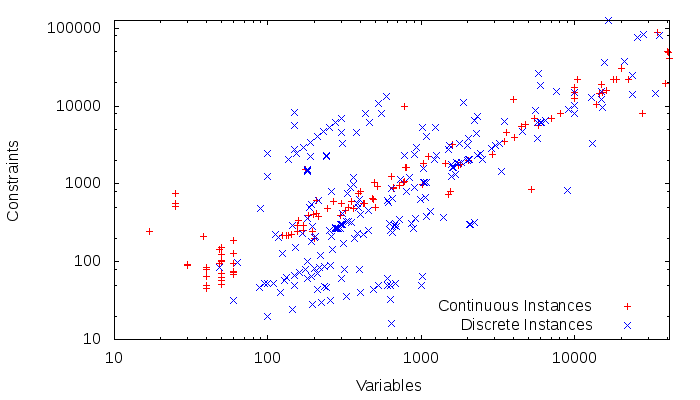
\includegraphics[width=0.85\textwidth]{pic_overview.png}
  \caption{Distribution of variables and constrains  of the qplib
instances \label{fig:distribution}}
\end{figure}

%Figure~\ref{fig:pic_var_small}, Figure~\ref{fig:pic_var_medium} and
Figure~\ref{fig:pic_var} 
describes how discrete and continuous
variables are distributed within the instances. The instances are
sorted accordingly to the total number of variables.
% and, for reason of
%readability, the graph is splitted in the three figures:
%Figure~\ref{fig:pic_var_small} describes the 100 smaller instances,
%Figure~\ref{fig:pic_var_medium} the 200 medium ones, and
%Figure~\ref{fig:pic_var_large} the 67 largest ones. 
For each instance we report the total number of variables with a ``$+$'', and the total number of discrete variables (binary or general integer) with a ``$\times$''. The pictures clearly show that instances with different percentages of integer and continuous variables are present in the library, and well distributed across the whole spectrum of variable sizes.

%%%%%%%%%%%%%%%%%%%%%%%%%%%%%%%
\begin{figure}\centering
  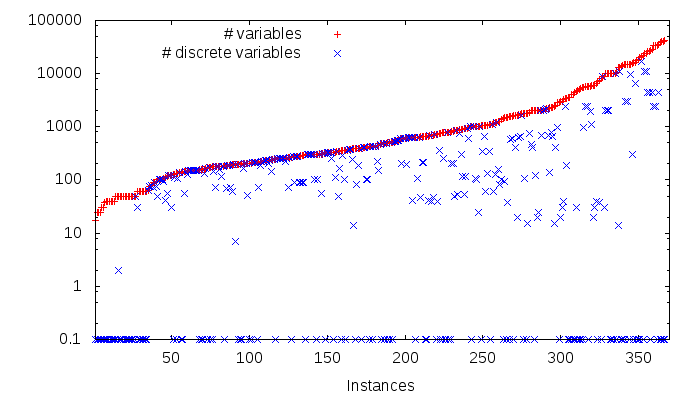
\includegraphics[width=0.85\textwidth]{pic_var.png}
  \caption{Number of variables \label{fig:pic_var}}
\end{figure}

%\begin{figure}\centering
%  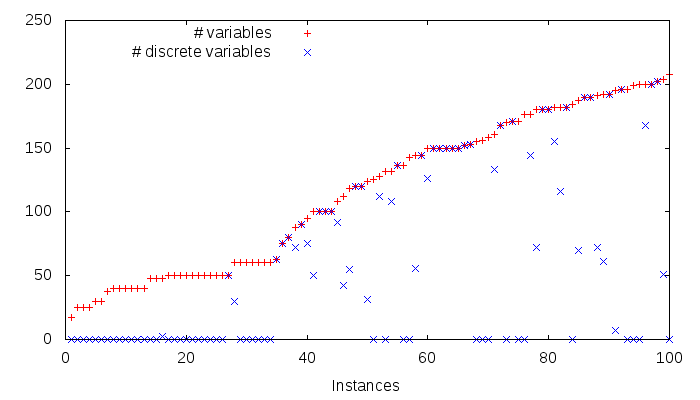
\includegraphics[width=0.85\textwidth]{pic_var_small.png}
%  \caption{Number of variables (a) \label{fig:pic_var_small}}
%\end{figure}
%
%\begin{figure}\centering
%  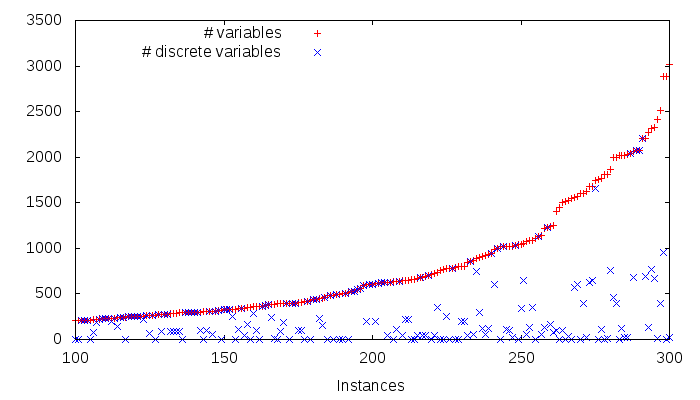
\includegraphics[width=0.85\textwidth]{pic_var_medium.png}
%  \caption{Number of variables (b) \label{fig:pic_var_medium}}
%\end{figure}
%
%\begin{figure}\centering
%  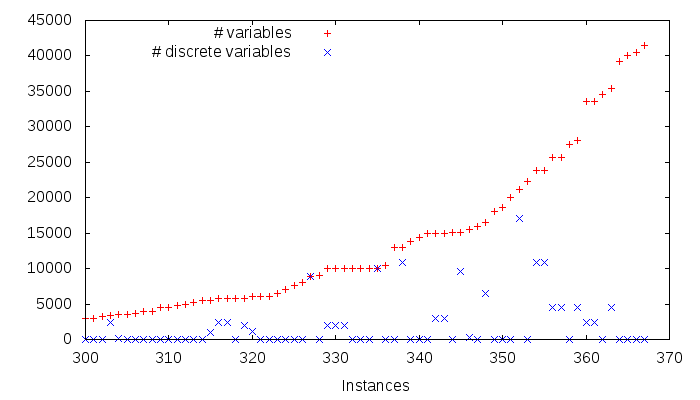
\includegraphics[width=0.85\textwidth]{pic_var_big.png}
%  \caption{Number of variables (c) \label{fig:pic_var_large}}
%\end{figure}

Similarly, Figures~\ref{fig:pic_constr} 
%Figure~\ref{fig:pic_constr_medium}
%and Figure~\ref{fig:pic_constr_big} 
describes how linear and quadratic
constraints are distributed within the instances. The instances are sorted
accordingly to the total number of constraints
% and divided in the same manner as for Figures~\ref{fig:pic_var_small}--\ref{fig:pic_var_large}.
For each instances we report the total number of constraints with a ``$+$''
and the total number of (either convex of nonconvex) quadratic constraints
with a ``$\times$''. Also in this case, different percentages of linear and
quadratic constraints are present and well-distributed across the spectrum
of constraint sizes, although both medium- and large-size instances show a
prevalence of lower percentages of quadratic constraints. In particular,
from Figure~\ref{fig:pic_constr} we learn that while the maximum number
of linear constraints exceeds 100000, the maximum number of quadratic
constraints tops up at around 10000. This is, however, reasonable, considering
how quadratic constraints can, in general, be expected to be much more
computationally challenging than linear ones, especially if nonconvex.

%%%%%%%%%%%%%%%%%%%%%%%%%%%%%%%%%%%%%%%
\begin{figure}\centering
  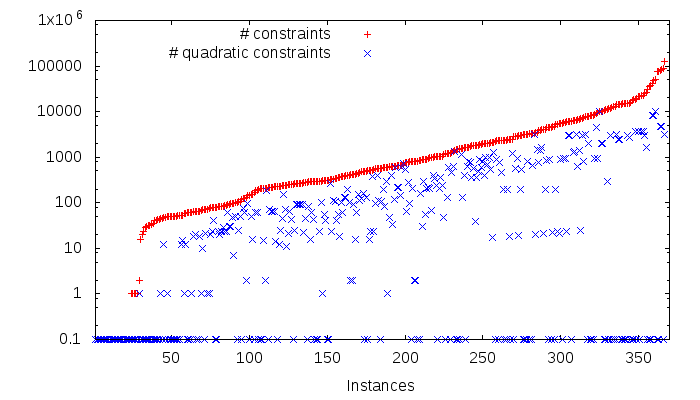
\includegraphics[width=0.85\textwidth]{pic_constr.png}
  \caption{Number of constraints \label{fig:pic_constr}}
\end{figure}

%\begin{figure}\centering
%  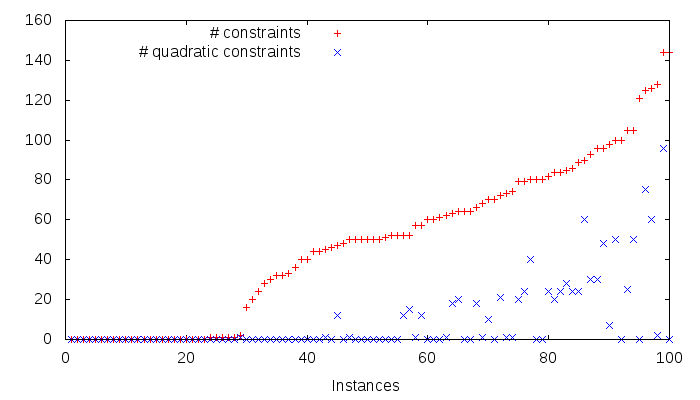
\includegraphics[width=0.85\textwidth]{pic_constr_small.png}
%  \caption{Number of constraints (a) \label{fig:pic_constr_small}}
%\end{figure}
%
%\begin{figure}\centering
%  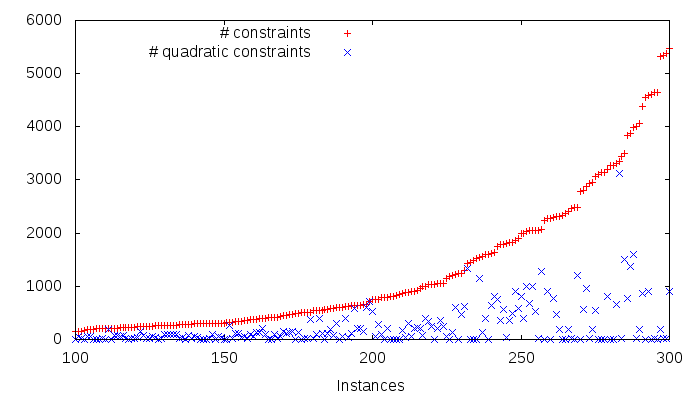
\includegraphics[width=0.85\textwidth]{pic_constr_medium.png}
%  \caption{Number of constraints (b) \label{fig:pic_constr_medium}}
%\end{figure}
%
%\begin{figure}\centering
%  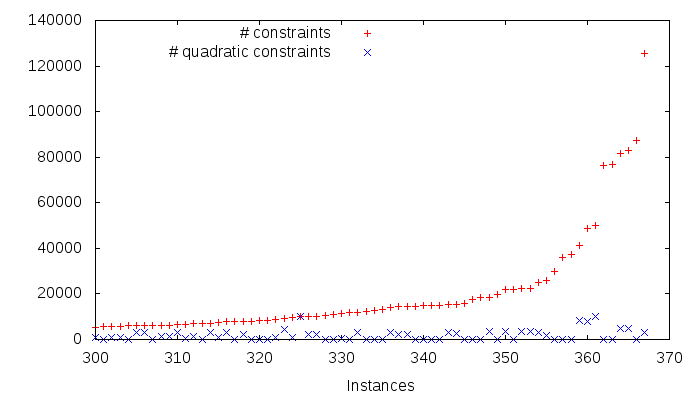
\includegraphics[width=0.85\textwidth]{pic_constr_big.png}
%  \caption{Number of constraints (c) \label{fig:pic_constr_big}}
%\end{figure}

Figure~\ref{fig:pic_conv_constr} shows the instances with at least a quadratic constraints sorted according to the number of quadratic constraints (vertical axis). For each instances we report the total number of constraints with a ``$+$''
and the total number of nonconvex quadratic constraints
with a ``$\times$''.

\begin{figure}\centering
  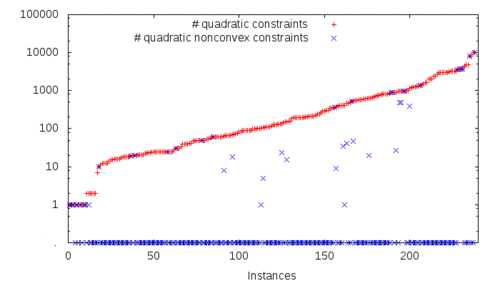
\includegraphics[width=0.85\textwidth]{pic_quad_conv_vs_nonconv.png}
  \caption{Quadratic constraints \label{fig:pic_conv_constr}}
\end{figure}





Speaking of nonconvexity, Figure~\ref{fig:pic_neg_eig} focuses on
the instances with a quadratic objective function, ordered by the
the percentage of negative eigenvalues (vertical axis). Although
almost all percentages are represented, the instances are mostly
clustered around two values. About 25\% of the instances are convex,
i.e., they have 0\% of negative eigenvalues. Among the others, a vast
majority have around 50\% of negative eigenvalues. However, instances
with high or low percentages of negative eigenvalues are present.

\begin{figure}\centering
  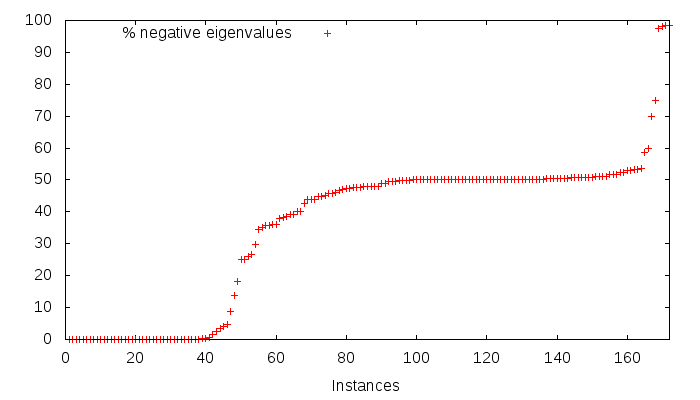
\includegraphics[width=0.85\textwidth]{pic_neg_eig.png}
  \caption{Negative eigenvalues \label{fig:pic_neg_eig}}
\end{figure}

Similarly, Figure~\ref{fig:pic_density} shows the instances with a
quadratic objective function sorted according to the density of the
$Q^0$ matrix (vertical axis). The majority of the instances have either
a very low or a rather high density: indeed, about 30\% of the instances
have density smaller that 5\%, and about 30\% of the instances have
density larger that 50\%. However, also intermediate values are present. 

\begin{figure}\centering
  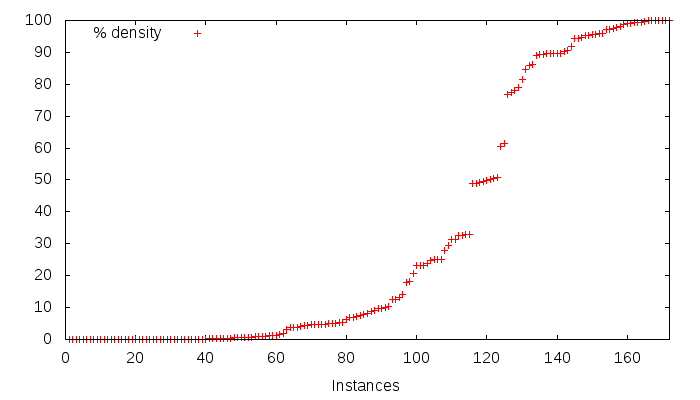
\includegraphics[width=0.85\textwidth]{pic_density.png}
  \caption{Density \label{fig:pic_density}}
\end{figure}


Additional details on the instance features can be found in \S~\ref{sec:instance_details}.
%- - - - - - - - - - - - - - - - - - - - - - - - - - - - - - - - - - - -
%- - - - - - - - - - - - - - - - - - - - - - - - - - - - - - - - - - - -
%  End QPLIB-3.tex
%- - - - - - - - - - - - - - - - - - - - - - - - - - - - - - - - - - - -
%- - - - - - - - - - - - - - - - - - - - - - - - - - - - - - - - - - - -


%- - - - - - - - - - - - - - - - - - - - - - - - - - - - - - - - - - - -

%- - - - - - - - - - - - - - - - - - - - - - - - - - - - - - - - - - - -

%%- - - - - - - - - - - - - - - - - - - - - - - - - - - - - - - - - - - -
%%- - - - - - - - - - - - - - - - - - - - - - - - - - - - - - - - - - - -
%%  QPLIB-4.tex
%%- - - - - - - - - - - - - - - - - - - - - - - - - - - - - - - - - - - -
%%- - - - - - - - - - - - - - - - - - - - - - - - - - - - - - - - - - - -
%
%\section{Software tools}\label{subsec:tools}
%
%%- - - - - - - - - - - - - - - - - - - - - - - - - - - - - - - - - - - -
%\subsection{instance translator}
%GAMS--LP--QPFORMAT
%\todo[inline]{TASK X : write }
%
%
%%- - - - - - - - - - - - - - - - - - - - - - - - - - - - - - - - - - - -
%\subsection{code that computes the features of an instance}
%\todo[inline]{TASK X : write }
%
%%- - - - - - - - - - - - - - - - - - - - - - - - - - - - - - - - - - - -
%\subsection{code that selects subsets of instances}
%\todo[inline]{TASK X : write }
%
%%- - - - - - - - - - - - - - - - - - - - - - - - - - - - - - - - - - - -
%\subsection{website, instance collector}
%Select subset or categories of instances (EXTRACT FROM THE LIBRARY A SUBSET OF INSTANCES WITH SPECIFIC CHARACTERISTICS)
%\todo[inline]{TASK X : write }
%
%The instances of QPLIB are publically accessible at the website \url{http://qplib.zib.de}.
%%
%Beyond links to the \texttt{gms} and \texttt{lp} format files, the website provides a rich set of metadata for each
%instance: the three letter problem classification, basic properties such as the number of variables and constraints of
%different types, the sense and curvature of the objective function, and information on the nonzero structure of the
%problem.
%%
%In addition, we display a visualization of the sparsity patterns of the Jacobian and the Hessian matrix of the
%Lagrangian function.  In the plots of the Jacobian nonzero pattern, the linear and nonlinear entries are distinguished
%by color.  Figure... shows an example for instance QPLIB...
%
%
%The entire set of instances can be explored in a searchable and sortable table of selected instance features: problem
%classification, convexity of the continuous relaxation, and number of variables, constraints, and nonzeros.
%%
%Finally, a statistics page displays diagrams on the composition of the library according to different criteria: the
%number instances according to problem type, variable types, convexity, number of variables and constraints, and density.
%%
%A table containing the relevant metadata for each instance can be downloaded in \texttt{csv} format and as spreadsheets
%such that researchers can easily compile their own subset of instances according to these statistics.
%
%
%The complete library can be downloaded as one archive, which contains the website for offline browsing and exploration.  
%%
%In the future, we plan to extend the website by the addition of contributor information and references to the literature.
%
%
%%- - - - - - - - - - - - - - - - - - - - - - - - - - - - - - - - - - - -
%\subsection{testing environment}
%RUN GAMS USING A SUBSET OF SOLVERS
%\todo[inline]{TASK X : write }
%
%%- - - - - - - - - - - - - - - - - - - - - - - - - - - - - - - - - - - -
%%- - - - - - - - - - - - - - - - - - - - - - - - - - - - - - - - - - - -
%%  End QPLIB-4.tex
%%- - - - - - - - - - - - - - - - - - - - - - - - - - - - - - - - - - - -
%%- - - - - - - - - - - - - - - - - - - - - - - - - - - - - - - - - - - -

%- - - - - - - - - - - - - - - - - - - - - - - - - - - - - - - - - - - -


%- - - - - - - - - - - - - - - - - - - - - - - - - - - - - - - - - - - -

\section{Conclusions}\label{sec:conclusions}

 This manuscript describes the first comprehensive library of instances for Quadratic Programming (QP). Since QP comprises  different and ``varied'' categories of problems, we propose a classification and then we describe the principal solution methods representing the state-of-the-art algorithms for QP.

We then describe the steps of the adopted process used to filter the gathered instances  in order to build the new library. The goals we purposed are of different natures and we tried to build a library which is computationally challenging and as broad as possible, i.e., it represents the largest possible categories of QP problems. 

We want to stress once again that we intentionally avoid to perform a computational comparison of the performances of the different solvers. Our goal is instead to provide a common test-bed of instances for practitioners and researchers in the field. This new library will hopefully serve as a point of reference to test new ideas and algorithms for QP problems.


%- - - - - - - - - - - - - - - - - - - - - - - - - - - - - - - - - - - -


%- - - - - - - - - - - - - - - - - - - - - - - - - - - - - - - - - - - -
%- - - - - - - - - - - - - - - - - - - - - - - - - - - - - - - - - - - -
\section{Acknowledgements}

%- - - - - - - - - - - - - - - - - - - - - - - - - - - - - - - - - - - -
%- - - - - - - - - - - - - - - - - - - - - - - - - - - - - - - - - - - -

\bibliography{biblio}

\ifMPC
 \bibliographystyle{spmpsci}
\else
 \bibliographystyle{plain}
\fi

%- - - - - - - - - - - - - - - - - - - - - - - - - - - - - - - - - - - -
%- - - - - - - - - - - - - - - - - - - - - - - - - - - - - - - - - - - -
\appendix

%- - - - - - - - - - - - - - - - - - - - - - - - - - - - - - - - - - - -
%- - - - - - - - - - - - - - - - - - - - - - - - - - - - - - - - - - - -
%  Appendix.tex
%- - - - - - - - - - - - - - - - - - - - - - - - - - - - - - - - - - - -
%- - - - - - - - - - - - - - - - - - - - - - - - - - - - - - - - - - - -

\section*{Appendix}\label{sec:appendix}

In this Appendix we provide detailed data on all the instances of the final library. This is done in Tables \ref{tab:A1}--\ref{tab:A10} for \emph{discrete} instances (*\{B,M,I,G\}*) and in Tables \ref{tab:B1}--\ref{tab:B5} for \emph{continuous} ones (*C*). In the former, the features of the instances are described by three sets of columns. The first (``\% eig'') describes the objective function by reporting the fraction of eigenvalues of $Q^0$ that are negative: a positive number implies that $Q^0$ is not SDP (hence, the instance is a Q**), ``0.000'' implies that $Q^0$ is SDP (hence, the instance is a C**), a blank implies that $Q^0 = 0$, i.e., the objective function is linear (hence, the instance is a L**). The following three columns describe the variables by reporting the number of binary ones (``\# bin''), general integer ones (``\# int''), and continuous ones (``\# cont''). Finally, the last three columns describe the constraints reporting the number of linear ones (``\# lin''), nonconvex quadratic ones (``\# quad''), and convex quadratic ones (``\# conv''). Tables \ref{tab:B1}--\ref{tab:B5} are similarly structured except that all variables are continuous, and hence only one column is present.

\begin{table}
 \centering
 %\scriptsize
 \setlength{\tabcolsep}{7pt}
 \renewcommand \arraystretch{1}
\begin{tabular}{lrrrrrrrrrrrr}
\toprule

	&		&		&	&	\multicolumn{3}{c}{Variables}					&	&	\multicolumn{4}{c}{Constraints}							\\
\cmidrule(lr){5-7} \cmidrule(lr){9-12}							 														
name	&	\% eig	&	\% dens	&	&	\# bin	&	\# int 	&	\# cont 	&	&	\# lin 	&	\# quad 	&	\# conv 	&	\# box	\\
\cmidrule(lr){5-7} \cmidrule(lr){9-12}																					

qplib\_1	&	2e-1	&	2e-1	&	&	30	&	0	&	30	&	&	32	&	0	&	0	&	30	\\
qplib\_2	&	3e-1	&	2e-1	&	&	50	&	0	&	50	&	&	52	&	0	&	0	&	50	\\
qplib\_3	&	5e-1	&	3e-1	&	&	90	&	0	&	0	&	&	1	&	0	&	0	&	90	\\
qplib\_4	&	5e-1	&	5e-1	&	&	100	&	0	&	0	&	&	1	&	0	&	0	&	100	\\
qplib\_5	&	5e-1	&	5e-1	&	&	90	&	0	&	0	&	&	1	&	0	&	0	&	90	\\
qplib\_6	&	5e-1	&	7e-1	&	&	100	&	0	&	0	&	&	1	&	0	&	0	&	100	\\
qplib\_7	&	5e-1	&	5e-1	&	&	70	&	0	&	0	&	&	1	&	0	&	0	&	70	\\
qplib\_8	&	5e-1	&	9e-1	&	&	90	&	0	&	0	&	&	1	&	0	&	0	&	90	\\
qplib\_9	&	4e-1	&	7e-1	&	&	50	&	0	&	0	&	&	1	&	0	&	0	&	50	\\
qplib\_10	&	5e-1	&	7e-1	&	&	80	&	0	&	0	&	&	1	&	0	&	0	&	80	\\
qplib\_11	&	5e-1	&	9e-1	&	&	80	&	0	&	0	&	&	1	&	0	&	0	&	80	\\
qplib\_12	&	5e-1	&	1e-1	&	&	144	&	0	&	0	&	&	24	&	0	&	0	&	144	\\
qplib\_13	&	3e-1	&	1e-2	&	&	536	&	0	&	0	&	&	138	&	0	&	0	&	536	\\
qplib\_14	&	5e-1	&	1e-2	&	&	750	&	0	&	0	&	&	253	&	0	&	0	&	750	\\
qplib\_15	&	5e-1	&	4e-2	&	&	400	&	0	&	0	&	&	104	&	0	&	0	&	400	\\
qplib\_16	&	5e-1	&	4e-2	&	&	300	&	0	&	0	&	&	103	&	0	&	0	&	300	\\
qplib\_17	&	5e-1	&	3e-2	&	&	300	&	0	&	0	&	&	103	&	0	&	0	&	300	\\
qplib\_18	&	5e-1	&	3e-2	&	&	300	&	0	&	0	&	&	103	&	0	&	0	&	300	\\
qplib\_19	&	2e-1	&	1e-2	&	&	402	&	0	&	0	&	&	137	&	0	&	0	&	402	\\
qplib\_20	&	5e-1	&	2e-2	&	&	496	&	0	&	0	&	&	128	&	0	&	0	&	496	\\
qplib\_21	&	5e-1	&	3e-2	&	&	300	&	0	&	0	&	&	103	&	0	&	0	&	300	\\
qplib\_22	&	5e-1	&	3e-2	&	&	400	&	0	&	0	&	&	104	&	0	&	0	&	400	\\
qplib\_23	&	5e-1	&	4e-2	&	&	400	&	0	&	0	&	&	104	&	0	&	0	&	400	\\
qplib\_24	&	5e-1	&	3e-2	&	&	400	&	0	&	0	&	&	104	&	0	&	0	&	400	\\
qplib\_25	&	4e-1	&	6e-3	&	&	1056	&	0	&	0	&	&	355	&	0	&	0	&	1056	\\
qplib\_26	&	5e-1	&	3e-2	&	&	400	&	0	&	0	&	&	104	&	0	&	0	&	400	\\
qplib\_27	&	3e-1	&	1e-2	&	&	670	&	0	&	0	&	&	139	&	0	&	0	&	670	\\
qplib\_28	&	4e-1	&	2e-2	&	&	372	&	0	&	0	&	&	127	&	0	&	0	&	372	\\
qplib\_29	&	5e-1	&	4e-2	&	&	372	&	0	&	0	&	&	127	&	0	&	0	&	372	\\
qplib\_30	&	5e-1	&	9e-1	&	&	50	&	0	&	0	&	&	1	&	0	&	0	&	50	\\
qplib\_31	&	6e-1	&	1e+0	&	&	50	&	0	&	0	&	&	1	&	0	&	0	&	50	\\
qplib\_32	&	5e-1	&	2e-1	&	&	50	&	0	&	0	&	&	1	&	0	&	0	&	50	\\
qplib\_33	&	5e-1	&	7e-1	&	&	50	&	0	&	0	&	&	1	&	0	&	0	&	50	\\
qplib\_34	&	5e-1	&	2e-1	&	&	75	&	0	&	0	&	&	1	&	0	&	0	&	75	\\
qplib\_35	&	5e-1	&	9e-1	&	&	75	&	0	&	0	&	&	1	&	0	&	0	&	75	\\
qplib\_36	&	6e-1	&	9e-1	&	&	75	&	0	&	0	&	&	1	&	0	&	0	&	75	\\
qplib\_37	&	5e-1	&	1e+0	&	&	75	&	0	&	0	&	&	1	&	0	&	0	&	75	\\
qplib\_38	&	5e-1	&	7e-1	&	&	75	&	0	&	0	&	&	1	&	0	&	0	&	75	\\
qplib\_39	&	5e-1	&	7e-1	&	&	50	&	0	&	0	&	&	1	&	0	&	0	&	50	\\
qplib\_40	&	6e-1	&	9e-1	&	&	75	&	0	&	0	&	&	1	&	0	&	0	&	75	\\
qplib\_41	&	5e-1	&	9e-1	&	&	50	&	0	&	0	&	&	1	&	0	&	0	&	50	\\
qplib\_42	&	5e-1	&	9e-1	&	&	75	&	0	&	0	&	&	1	&	0	&	0	&	75	\\
qplib\_43	&	6e-1	&	1e+0	&	&	75	&	0	&	0	&	&	1	&	0	&	0	&	75	\\
qplib\_44	&	5e-1	&	2e-1	&	&	50	&	0	&	0	&	&	1	&	0	&	0	&	50	\\
qplib\_45	&	5e-1	&	7e-1	&	&	75	&	0	&	0	&	&	1	&	0	&	0	&	75	\\
qplib\_46	&		&		&	&	9600	&	0	&	6497	&	&	8417	&	960	&	480	&	10337	\\
qplib\_47	&		&		&	&	87	&	0	&	205	&	&	730	&	48	&	0	&	246	\\
qplib\_48	&		&		&	&	87	&	0	&	299	&	&	1002	&	96	&	0	&	294	\\
qplib\_49	&		&		&	&	104	&	0	&	328	&	&	1032	&	96	&	0	&	336	\\
qplib\_50	&		&		&	&	124	&	0	&	412	&	&	1508	&	128	&	0	&	408	\\
qplib\_51	&		&		&	&	304	&	0	&	760	&	&	2868	&	192	&	0	&	872	\\
qplib\_52	&		&		&	&	760	&	0	&	2220	&	&	8196	&	640	&	0	&	2340	\\
qplib\_53	&		&		&	&	760	&	0	&	2540	&	&	9348	&	800	&	0	&	2500	\\
qplib\_54	&		&		&	&	2040	&	0	&	5500	&	&	28256	&	1600	&	0	&	5940	\\
qplib\_55	&		&		&	&	792	&	0	&	1436	&	&	11924	&	288	&	0	&	1940	\\
qplib\_56	&		&		&	&	6520	&	0	&	13340	&	&	128792	&	3200	&	0	&	16660	\\
qplib\_57	&		&		&	&	187	&	0	&	240	&	&	423	&	33	&	0	&	394	\\
qplib\_58	&		&		&	&	55	&	0	&	78	&	&	141	&	15	&	0	&	118	\\
qplib\_59	&	0e+0	&	3e-4	&	&	720	&	0	&	240	&	&	5329	&	0	&	0	&	730	\\
qplib\_60	&	5e-1	&	1e-1	&	&	250	&	0	&	0	&	&	1	&	0	&	0	&	250	\\




\bottomrule

\end{tabular}  
\label{tab:A1}
\caption{Discrete Instance Feature 1-60} 

\end{table}

%%%%%%%%%%%%%%%%%%%%%%%%%%%%%%%%%%%%%%%%%%%%%%%%%%%%%%%%%
%%%%%%%%%%%%%%%%%%%%%%%%%%%%%%%%%%%%%%%%%%%%%%%%%%%%%%%%%
%%%%%%%%%%%%%%%%%%%%%%%%%%%%%%%%%%%%%%%%%%%%%%%%%%%%%%%%%
\begin{table}
 \centering
 %\scriptsize
 \setlength{\tabcolsep}{7pt}
 \renewcommand \arraystretch{1}
\begin{tabular}{lrrrrrrrrrrrr}
\toprule

	&		&		&	&	\multicolumn{3}{c}{Variables}					&	&	\multicolumn{4}{c}{Constraints}							\\
\cmidrule(lr){5-7} \cmidrule(lr){9-12}							 														
name	&	\% eig	&	\% dens	&	&	\# bin	&	\# int 	&	\# cont 	&	&	\# lin 	&	\# quad 	&	\# conv 	&	\# box	\\
\cmidrule(lr){5-7} \cmidrule(lr){9-12}																					
qplib\_61	&	5e-1	&	1e-1	&	&	250	&	0	&	0	&	&	1	&	0	&	0	&	250	\\
qplib\_62	&	5e-1	&	1e-1	&	&	250	&	0	&	0	&	&	1	&	0	&	0	&	250	\\
qplib\_63	&	5e-1	&	1e-1	&	&	250	&	0	&	0	&	&	1	&	0	&	0	&	250	\\
qplib\_64	&	5e-1	&	1e-1	&	&	250	&	0	&	0	&	&	1	&	0	&	0	&	250	\\
qplib\_65	&	3e-1	&	6e-2	&	&	152	&	0	&	17	&	&	153	&	16	&	0	&	152	\\
qplib\_66	&	4e-1	&	5e-2	&	&	252	&	0	&	22	&	&	253	&	21	&	0	&	252	\\
qplib\_67	&	4e-1	&	4e-2	&	&	275	&	0	&	23	&	&	276	&	22	&	0	&	275	\\
qplib\_68	&	4e-1	&	4e-2	&	&	299	&	0	&	24	&	&	300	&	23	&	0	&	299	\\
qplib\_69	&	4e-1	&	4e-2	&	&	299	&	0	&	24	&	&	300	&	23	&	0	&	299	\\
qplib\_70	&	4e-1	&	4e-2	&	&	324	&	0	&	25	&	&	325	&	24	&	0	&	324	\\
qplib\_71	&	4e-1	&	4e-2	&	&	324	&	0	&	25	&	&	325	&	24	&	0	&	324	\\
qplib\_72	&	4e-1	&	4e-2	&	&	324	&	0	&	25	&	&	325	&	24	&	0	&	324	\\
qplib\_73	&		&		&	&	136	&	0	&	17	&	&	2057	&	17	&	0	&	136	\\
qplib\_74	&		&		&	&	153	&	0	&	18	&	&	2466	&	18	&	0	&	153	\\
qplib\_75	&		&		&	&	153	&	0	&	18	&	&	2466	&	18	&	0	&	153	\\
qplib\_76	&		&		&	&	153	&	0	&	18	&	&	2466	&	18	&	0	&	153	\\
qplib\_77	&		&		&	&	171	&	0	&	19	&	&	2926	&	19	&	0	&	171	\\
qplib\_78	&		&		&	&	171	&	0	&	19	&	&	2926	&	19	&	0	&	171	\\
qplib\_79	&		&		&	&	171	&	0	&	19	&	&	2926	&	19	&	0	&	171	\\
qplib\_80	&		&		&	&	171	&	0	&	19	&	&	2926	&	19	&	0	&	171	\\
qplib\_81	&		&		&	&	171	&	0	&	19	&	&	2926	&	19	&	0	&	171	\\
qplib\_82	&		&		&	&	190	&	0	&	20	&	&	3440	&	20	&	0	&	190	\\
qplib\_83	&		&		&	&	190	&	0	&	20	&	&	3440	&	20	&	0	&	190	\\
qplib\_84	&		&		&	&	190	&	0	&	20	&	&	3440	&	20	&	0	&	190	\\
qplib\_85	&		&		&	&	190	&	0	&	20	&	&	3440	&	20	&	0	&	190	\\
qplib\_86	&		&		&	&	190	&	0	&	20	&	&	3440	&	20	&	0	&	190	\\
qplib\_87	&		&		&	&	190	&	0	&	20	&	&	3440	&	20	&	0	&	190	\\
qplib\_88	&		&		&	&	210	&	0	&	21	&	&	4011	&	21	&	0	&	210	\\
qplib\_89	&		&		&	&	210	&	0	&	21	&	&	4011	&	21	&	0	&	210	\\
qplib\_90	&		&		&	&	210	&	0	&	21	&	&	4011	&	21	&	0	&	210	\\
qplib\_91	&		&		&	&	231	&	0	&	22	&	&	4642	&	22	&	0	&	231	\\
qplib\_92	&		&		&	&	253	&	0	&	23	&	&	5336	&	23	&	0	&	253	\\
qplib\_93	&		&		&	&	253	&	0	&	23	&	&	5336	&	23	&	0	&	253	\\
qplib\_94	&		&		&	&	253	&	0	&	23	&	&	5336	&	23	&	0	&	253	\\
qplib\_95	&		&		&	&	276	&	0	&	24	&	&	6096	&	24	&	0	&	276	\\
qplib\_96	&		&		&	&	276	&	0	&	24	&	&	6096	&	24	&	0	&	276	\\
qplib\_97	&		&		&	&	300	&	0	&	25	&	&	6925	&	25	&	0	&	300	\\
qplib\_98	&		&		&	&	300	&	0	&	25	&	&	6925	&	25	&	0	&	300	\\
qplib\_99	&		&		&	&	300	&	0	&	25	&	&	6925	&	25	&	0	&	300	\\
qplib\_100	&		&		&	&	192	&	0	&	2	&	&	65	&	1	&	0	&	192	\\
qplib\_101	&		&		&	&	683	&	0	&	1376	&	&	1366	&	683	&	0	&	683	\\
qplib\_102	&		&		&	&	345	&	0	&	697	&	&	690	&	345	&	0	&	345	\\
qplib\_103	&		&		&	&	61	&	0	&	131	&	&	122	&	61	&	0	&	61	\\
qplib\_104	&		&		&	&	214	&	0	&	438	&	&	428	&	214	&	0	&	214	\\
qplib\_105	&		&		&	&	297	&	0	&	608	&	&	594	&	297	&	0	&	297	\\
qplib\_106	&		&		&	&	351	&	0	&	736	&	&	702	&	351	&	0	&	351	\\
qplib\_107	&		&		&	&	150	&	0	&	305	&	&	300	&	150	&	0	&	150	\\
qplib\_108	&		&		&	&	150	&	0	&	305	&	&	300	&	150	&	0	&	150	\\
qplib\_109	&		&		&	&	215	&	0	&	436	&	&	430	&	215	&	0	&	215	\\
qplib\_110	&		&		&	&	768	&	0	&	1545	&	&	1536	&	768	&	0	&	768	\\
qplib\_111	&		&		&	&	90	&	0	&	190	&	&	180	&	90	&	0	&	90	\\
qplib\_112	&		&		&	&	90	&	0	&	195	&	&	180	&	90	&	0	&	90	\\
qplib\_113	&		&		&	&	90	&	0	&	200	&	&	180	&	90	&	0	&	90	\\
qplib\_114	&		&		&	&	90	&	0	&	205	&	&	180	&	90	&	0	&	90	\\
qplib\_115	&		&		&	&	90	&	0	&	185	&	&	180	&	90	&	0	&	90	\\
qplib\_116	&		&		&	&	100	&	0	&	205	&	&	200	&	100	&	0	&	100	\\
qplib\_117	&		&		&	&	110	&	0	&	225	&	&	220	&	110	&	0	&	110	\\
qplib\_118	&		&		&	&	958	&	0	&	1926	&	&	1916	&	958	&	0	&	958	\\
qplib\_119	&		&		&	&	194	&	0	&	421	&	&	388	&	194	&	0	&	194	\\
qplib\_120	&		&		&	&	0	&	100	&	2	&	&	4	&	1	&	1	&	0	\\

		
		
		
\bottomrule

\end{tabular}  
\label{tab:A2}
\caption{Discrete Instance Feature 61-120} 

\end{table}
%%%%%%%%%%%%%%%%%%%%%%%%%%%%%%%%%%%%%%%%%%%%%%%%%%%%%%%%%
%%%%%%%%%%%%%%%%%%%%%%%%%%%%%%%%%%%%%%%%%%%%%%%%%%%%%%%%%
%%%%%%%%%%%%%%%%%%%%%%%%%%%%%%%%%%%%%%%%%%%%%%%%%%%%%%%%%
\begin{table}
 \centering
 %\scriptsize
 \setlength{\tabcolsep}{7pt}
 \renewcommand \arraystretch{1}
\begin{tabular}{lrrrrrrrrrrrr}
\toprule

		&		&		&	&	\multicolumn{3}{c}{Variables}					&	&	\multicolumn{4}{c}{Constraints}							\\
\cmidrule(lr){5-7} \cmidrule(lr){9-12}							 														
name	&	\% eig	&	\% dens	&	&	\# bin	&	\# int 	&	\# cont 	&	&	\# lin 	&	\# quad 	&	\# conv 	&	\# box	\\
\cmidrule(lr){5-7} \cmidrule(lr){9-12}																					



qplib\_121	&		&		&	&	0	&	100	&	2	&	&	4	&	1	&	1	&	0	\\
qplib\_122	&		&		&	&	0	&	100	&	2	&	&	4	&	1	&	1	&	0	\\
qplib\_123	&		&		&	&	0	&	100	&	2	&	&	4	&	1	&	1	&	0	\\
qplib\_124	&		&		&	&	0	&	100	&	2	&	&	4	&	1	&	1	&	0	\\
qplib\_125	&		&		&	&	0	&	100	&	2	&	&	4	&	1	&	1	&	0	\\
qplib\_126	&		&		&	&	0	&	100	&	2	&	&	4	&	1	&	1	&	0	\\
qplib\_127	&		&		&	&	595	&	0	&	2	&	&	13091	&	1	&	0	&	595	\\
qplib\_128	&		&		&	&	435	&	0	&	2	&	&	8121	&	1	&	0	&	435	\\
qplib\_129	&		&		&	&	240	&	0	&	2	&	&	2241	&	1	&	0	&	240	\\
qplib\_130	&		&		&	&	240	&	0	&	2	&	&	2241	&	1	&	0	&	240	\\
qplib\_131	&		&		&	&	240	&	0	&	2	&	&	2241	&	1	&	0	&	240	\\
qplib\_132	&		&		&	&	240	&	0	&	2	&	&	2241	&	1	&	0	&	240	\\
qplib\_133	&		&		&	&	147	&	0	&	95	&	&	2241	&	1	&	0	&	240	\\
qplib\_134	&		&		&	&	240	&	0	&	2	&	&	2241	&	1	&	0	&	240	\\
qplib\_135	&		&		&	&	240	&	0	&	2	&	&	2241	&	1	&	0	&	240	\\
qplib\_136	&		&		&	&	240	&	0	&	2	&	&	2241	&	1	&	0	&	240	\\
qplib\_137	&		&		&	&	240	&	0	&	2	&	&	2241	&	1	&	0	&	240	\\
qplib\_138	&		&		&	&	306	&	0	&	2	&	&	3265	&	1	&	0	&	306	\\
qplib\_139	&		&		&	&	306	&	0	&	2	&	&	3265	&	1	&	0	&	306	\\
qplib\_140	&		&		&	&	190	&	0	&	2	&	&	2281	&	1	&	0	&	190	\\
qplib\_141	&	0e+0	&	3e-4	&	&	28	&	0	&	477	&	&	576	&	0	&	0	&	56	\\
qplib\_142	&	5e-1	&	9e-1	&	&	676	&	0	&	0	&	&	52	&	0	&	0	&	676	\\
qplib\_143	&	4e-1	&	9e-1	&	&	196	&	0	&	0	&	&	28	&	0	&	0	&	196	\\
qplib\_144	&	6e-1	&	3e-1	&	&	256	&	0	&	0	&	&	32	&	0	&	0	&	256	\\
qplib\_145	&	5e-1	&	8e-1	&	&	100	&	0	&	0	&	&	20	&	0	&	0	&	100	\\
qplib\_146	&		&		&	&	42	&	0	&	86	&	&	211	&	14	&	0	&	58	\\
qplib\_147	&		&		&	&	42	&	0	&	86	&	&	211	&	14	&	0	&	58	\\
qplib\_148	&		&		&	&	25	&	0	&	38	&	&	31	&	26	&	26	&	30	\\
qplib\_149	&	1e-2	&	2e-4	&	&	0	&	2213	&	4191	&	&	483	&	0	&	0	&	2213	\\
qplib\_150	&	5e-1	&	6e-1	&	&	625	&	0	&	0	&	&	50	&	0	&	0	&	625	\\
qplib\_151	&	4e-1	&	2e-1	&	&	1024	&	0	&	0	&	&	64	&	0	&	0	&	1024	\\
qplib\_152	&	3e-1	&	1e-1	&	&	256	&	0	&	0	&	&	32	&	0	&	0	&	256	\\
qplib\_153	&	5e-2	&	1e-2	&	&	259	&	0	&	1	&	&	212	&	0	&	0	&	259	\\
qplib\_154	&		&		&	&	108	&	0	&	568	&	&	369	&	30	&	0	&	661	\\
qplib\_155	&	4e-1	&	9e-1	&	&	324	&	0	&	0	&	&	36	&	0	&	0	&	324	\\
qplib\_156	&	5e-1	&	7e-2	&	&	625	&	0	&	0	&	&	50	&	0	&	0	&	625	\\
qplib\_157	&		&		&	&	30	&	0	&	68	&	&	157	&	12	&	0	&	44	\\
qplib\_158	&		&		&	&	42	&	0	&	86	&	&	211	&	14	&	0	&	58	\\
qplib\_159	&	3e-3	&	2e-4	&	&	252	&	0	&	1499	&	&	1913	&	0	&	0	&	1714	\\
qplib\_160	&	5e-1	&	9e-1	&	&	625	&	0	&	0	&	&	50	&	0	&	0	&	625	\\
qplib\_161	&		&		&	&	56	&	0	&	106	&	&	273	&	16	&	0	&	74	\\
qplib\_162	&	0e+0	&	2e-2	&	&	150	&	0	&	1	&	&	68	&	0	&	0	&	151	\\
qplib\_163	&	5e-1	&	3e-1	&	&	225	&	0	&	0	&	&	30	&	0	&	0	&	225	\\
qplib\_164	&		&		&	&	2	&	0	&	33	&	&	31	&	6	&	0	&	29	\\
qplib\_165	&		&		&	&	25	&	0	&	368	&	&	298	&	24	&	0	&	120	\\
qplib\_166	&	7e-1	&	6e-1	&	&	256	&	0	&	0	&	&	32	&	0	&	0	&	256	\\
qplib\_167	&		&		&	&	72	&	0	&	128	&	&	343	&	18	&	0	&	92	\\
qplib\_168	&	5e-1	&	6e-1	&	&	484	&	0	&	0	&	&	44	&	0	&	0	&	484	\\
qplib\_169	&		&		&	&	42	&	0	&	86	&	&	211	&	14	&	0	&	58	\\
qplib\_170	&	5e-1	&	9e-1	&	&	225	&	0	&	0	&	&	30	&	0	&	0	&	225	\\
qplib\_171	&	2e-2	&	3e-3	&	&	256	&	0	&	256	&	&	296	&	0	&	0	&	256	\\
qplib\_172	&	5e-1	&	1e-1	&	&	1024	&	0	&	0	&	&	64	&	0	&	0	&	1024	\\
qplib\_173	&		&		&	&	24	&	0	&	189	&	&	213	&	48	&	30	&	40	\\
qplib\_174	&	5e-1	&	9e-1	&	&	2500	&	0	&	0	&	&	100	&	0	&	0	&	2500	\\
qplib\_175	&	5e-1	&	4e-1	&	&	144	&	0	&	0	&	&	24	&	0	&	0	&	144	\\
qplib\_176	&	2e-3	&	2e-4	&	&	48	&	0	&	792	&	&	1192	&	0	&	0	&	48	\\
qplib\_177	&	4e-1	&	8e-1	&	&	144	&	0	&	0	&	&	24	&	0	&	0	&	144	\\
qplib\_178	&	5e-1	&	9e-1	&	&	676	&	0	&	0	&	&	52	&	0	&	0	&	676	\\
qplib\_179	&	2e-2	&	4e-3	&	&	169	&	0	&	169	&	&	195	&	0	&	0	&	169	\\
qplib\_180	&	5e-1	&	1e-1	&	&	144	&	0	&	0	&	&	24	&	0	&	0	&	144	\\



\bottomrule

\end{tabular}  
\label{tab:A3}
\caption{Discrete  Instance Feature 121-180} 

\end{table}

%%%%%%%%%%%%%%%%%%%%%%%%%%%%%%%%%%%%%%%%%%%%%%%%%%%%%%%%%
%%%%%%%%%%%%%%%%%%%%%%%%%%%%%%%%%%%%%%%%%%%%%%%%%%%%%%%%%
%%%%%%%%%%%%%%%%%%%%%%%%%%%%%%%%%%%%%%%%%%%%%%%%%%%%%%%%%
\begin{table}
 \centering
 %\scriptsize
 \setlength{\tabcolsep}{7pt}
 \renewcommand \arraystretch{1}
\begin{tabular}{lrrrrrrrrrrrr}
\toprule

		&		&		&	&	\multicolumn{3}{c}{Variables}					&	&	\multicolumn{4}{c}{Constraints}							\\
\cmidrule(lr){5-7} \cmidrule(lr){9-12}							 														
name	&	\% eig	&	\% dens	&	&	\# bin	&	\# int 	&	\# cont 	&	&	\# lin 	&	\# quad 	&	\# conv 	&	\# box	\\
\cmidrule(lr){5-7} \cmidrule(lr){9-12}																					


qplib\_181	&	0e+0	&	1e-4	&	&	17136	&	0	&	3988	&	&	36703	&	0	&	0	&	17912	\\
qplib\_182	&	5e-1	&	9e-1	&	&	1225	&	0	&	0	&	&	70	&	0	&	0	&	1225	\\
qplib\_183	&	6e-1	&	5e-1	&	&	256	&	0	&	0	&	&	32	&	0	&	0	&	256	\\
qplib\_184	&	3e-1	&	1e-1	&	&	256	&	0	&	0	&	&	32	&	0	&	0	&	256	\\
qplib\_185	&		&		&	&	84	&	0	&	328	&	&	200	&	16	&	0	&	406	\\
qplib\_186	&		&		&	&	25	&	0	&	574	&	&	378	&	150	&	0	&	180	\\
qplib\_187	&		&		&	&	56	&	0	&	273	&	&	170	&	16	&	0	&	321	\\
qplib\_188	&	5e-1	&	6e-1	&	&	256	&	0	&	0	&	&	32	&	0	&	0	&	256	\\
qplib\_189	&	5e-1	&	1e-1	&	&	225	&	0	&	0	&	&	30	&	0	&	0	&	225	\\
qplib\_190	&	5e-1	&	9e-1	&	&	676	&	0	&	0	&	&	52	&	0	&	0	&	676	\\
qplib\_191	&	5e-1	&	3e-1	&	&	1024	&	0	&	0	&	&	64	&	0	&	0	&	1024	\\
qplib\_192	&	4e-1	&	8e-1	&	&	144	&	0	&	0	&	&	24	&	0	&	0	&	144	\\
qplib\_193	&	3e-2	&	3e-4	&	&	8904	&	0	&	0	&	&	823	&	0	&	0	&	8904	\\
qplib\_194	&	5e-1	&	8e-1	&	&	144	&	0	&	0	&	&	24	&	0	&	0	&	144	\\
qplib\_195	&	5e-1	&	9e-2	&	&	400	&	0	&	0	&	&	40	&	0	&	0	&	400	\\
qplib\_196	&		&		&	&	42	&	0	&	86	&	&	211	&	14	&	0	&	58	\\
qplib\_197	&		&		&	&	200	&	56	&	136	&	&	687	&	64	&	8	&	264	\\
qplib\_198	&		&		&	&	90	&	0	&	2	&	&	481	&	1	&	0	&	90	\\
qplib\_199	&	0e+0	&	2e-3	&	&	10	&	0	&	400	&	&	440	&	0	&	0	&	10	\\
qplib\_200	&		&		&	&	10920	&	0	&	4180	&	&	2299	&	3130	&	0	&	10920	\\
qplib\_201	&		&		&	&	80	&	0	&	104	&	&	1457	&	1	&	0	&	182	\\
qplib\_202	&		&		&	&	201	&	0	&	603	&	&	605	&	2	&	0	&	402	\\
qplib\_203	&		&		&	&	496	&	0	&	2	&	&	1	&	1	&	0	&	496	\\
qplib\_204	&	0e+0	&	1e-3	&	&	25	&	0	&	625	&	&	650	&	0	&	0	&	25	\\
qplib\_205	&		&		&	&	2450	&	0	&	1782	&	&	990	&	1332	&	0	&	2450	\\
qplib\_206	&		&		&	&	101	&	0	&	303	&	&	305	&	2	&	0	&	202	\\
qplib\_207	&		&		&	&	105	&	0	&	977	&	&	4813	&	54	&	0	&	927	\\
qplib\_208	&		&		&	&	2450	&	0	&	4134	&	&	5792	&	1283	&	392	&	2450	\\
qplib\_209	&		&		&	&	87	&	0	&	157	&	&	622	&	24	&	0	&	222	\\
qplib\_210	&		&		&	&	126	&	0	&	2108	&	&	4104	&	882	&	0	&	720	\\
qplib\_211	&		&		&	&	15	&	0	&	1800	&	&	960	&	900	&	0	&	15	\\
qplib\_212	&		&		&	&	352	&	0	&	430	&	&	768	&	48	&	0	&	734	\\
qplib\_213	&		&		&	&	64	&	0	&	769	&	&	1739	&	256	&	0	&	286	\\
qplib\_214	&	0e+0	&	2e-4	&	&	180	&	0	&	111	&	&	406	&	0	&	0	&	200	\\
qplib\_215	&		&		&	&	112	&	0	&	1677	&	&	3405	&	672	&	0	&	571	\\
qplib\_216	&	5e-1	&	9e-1	&	&	600	&	0	&	0	&	&	50	&	0	&	0	&	600	\\
qplib\_217	&		&		&	&	42	&	0	&	630	&	&	254	&	42	&	0	&	42	\\
qplib\_218	&		&		&	&	155	&	0	&	29	&	&	1457	&	1	&	0	&	182	\\
qplib\_219	&		&		&	&	132	&	0	&	1141	&	&	3445	&	192	&	0	&	829	\\
qplib\_220	&	5e-1	&	5e-4	&	&	0	&	1662	&	126	&	&	91	&	39	&	0	&	1710	\\
qplib\_221	&		&		&	&	38	&	0	&	128	&	&	213	&	34	&	0	&	97	\\
qplib\_222	&		&		&	&	40	&	0	&	472	&	&	1016	&	160	&	0	&	172	\\
qplib\_223	&		&		&	&	38	&	0	&	2033	&	&	2253	&	544	&	0	&	982	\\
qplib\_224	&		&		&	&	0	&	100	&	2	&	&	4	&	1	&	1	&	0	\\
qplib\_225	&		&		&	&	240	&	0	&	168	&	&	201	&	25	&	0	&	269	\\
qplib\_226	&	5e-1	&	9e-1	&	&	525	&	0	&	0	&	&	50	&	0	&	0	&	525	\\
qplib\_227	&		&		&	&	10	&	0	&	800	&	&	440	&	400	&	0	&	10	\\
qplib\_228	&		&		&	&	9	&	0	&	60	&	&	82	&	20	&	0	&	49	\\
qplib\_229	&	5e-1	&	2e-2	&	&	243	&	0	&	0	&	&	81	&	0	&	0	&	243	\\
qplib\_230	&	0e+0	&	1e-3	&	&	20	&	0	&	800	&	&	840	&	0	&	0	&	20	\\
qplib\_231	&		&		&	&	70	&	0	&	1140	&	&	2102	&	490	&	0	&	376	\\
qplib\_232	&		&		&	&	70	&	0	&	1026	&	&	1998	&	420	&	0	&	340	\\
qplib\_233	&		&		&	&	44	&	0	&	48	&	&	481	&	1	&	0	&	90	\\
qplib\_234	&	0e+0	&	2e-6	&	&	462	&	0	&	1536	&	&	3137	&	0	&	0	&	462	\\
qplib\_235	&		&		&	&	650	&	0	&	1416	&	&	1709	&	583	&	175	&	650	\\
qplib\_236	&	0e+0	&	4e-2	&	&	14	&	0	&	19	&	&	28	&	0	&	0	&	26	\\
qplib\_237	&		&		&	&	36	&	0	&	78	&	&	213	&	12	&	0	&	102	\\
qplib\_238	&	0e+0	&	1e-3	&	&	15	&	0	&	900	&	&	960	&	0	&	0	&	15	\\
qplib\_239	&		&		&	&	182	&	0	&	2	&	&	1457	&	1	&	0	&	182	\\
qplib\_240	&	1e-1	&	2e-1	&	&	14	&	0	&	370	&	&	556	&	0	&	0	&	14	\\


\bottomrule

\end{tabular}  
\label{tab:A4}
\caption{Discrete  Instance Feature 181-240} 

\end{table}

%%%%%%%%%%%%%%%%%%%%%%%%%%%%%%%%%%%%%%%%%%%%%%%%%%%%%%%%%
%%%%%%%%%%%%%%%%%%%%%%%%%%%%%%%%%%%%%%%%%%%%%%%%%%%%%%%%%
%%%%%%%%%%%%%%%%%%%%%%%%%%%%%%%%%%%%%%%%%%%%%%%%%%%%%%%%%
\begin{table}
 \centering
 %\scriptsize
 \setlength{\tabcolsep}{7pt}
 \renewcommand \arraystretch{1}
\begin{tabular}{lrrrrrrrrrrrr}
\toprule

		&		&		&	&	\multicolumn{3}{c}{Variables}					&	&	\multicolumn{4}{c}{Constraints}							\\
\cmidrule(lr){5-7} \cmidrule(lr){9-12}							 														
name	&	\% eig	&	\% dens	&	&	\# bin	&	\# int 	&	\# cont 	&	&	\# lin 	&	\# quad 	&	\# conv 	&	\# box	\\
\cmidrule(lr){5-7} \cmidrule(lr){9-12}																					

				qplib\_241	&	5e-1	&	9e-1	&	&	525	&	0	&	0	&	&	50	&	0	&	0	&	525	\\
qplib\_242	&		&		&	&	0	&	100	&	2	&	&	4	&	1	&	1	&	0	\\
qplib\_243	&		&		&	&	126	&	0	&	1894	&	&	3908	&	756	&	0	&	648	\\
qplib\_244	&	6e-1	&	1e+0	&	&	50	&	0	&	0	&	&	1	&	0	&	0	&	50	\\
qplib\_245	&		&		&	&	12	&	36	&	3	&	&	54	&	3	&	0	&	48	\\
qplib\_246	&		&		&	&	7	&	56	&	7	&	&	42	&	7	&	0	&	63	\\
qplib\_247	&		&		&	&	276	&	0	&	2	&	&	1	&	1	&	0	&	276	\\
qplib\_248	&	6e-2	&	2e-1	&	&	12	&	0	&	54	&	&	33	&	0	&	0	&	66	\\
qplib\_249	&		&		&	&	182	&	0	&	2	&	&	1457	&	1	&	0	&	182	\\
qplib\_250	&		&		&	&	24	&	0	&	57	&	&	38	&	27	&	0	&	24	\\
qplib\_251	&		&		&	&	0	&	100	&	2	&	&	4	&	1	&	1	&	0	\\
qplib\_252	&		&		&	&	44	&	0	&	16	&	&	28	&	12	&	0	&	44	\\
qplib\_253	&		&		&	&	114	&	0	&	2114	&	&	3854	&	912	&	0	&	725	\\
qplib\_254	&		&		&	&	0	&	100	&	2	&	&	4	&	1	&	1	&	0	\\
qplib\_255	&	5e-1	&	4e-2	&	&	144	&	0	&	0	&	&	48	&	0	&	0	&	144	\\
qplib\_256	&		&		&	&	10	&	0	&	1600	&	&	880	&	800	&	0	&	10	\\
qplib\_257	&		&		&	&	108	&	0	&	24	&	&	45	&	18	&	0	&	108	\\
qplib\_258	&		&		&	&	184	&	0	&	32	&	&	60	&	24	&	0	&	184	\\
qplib\_259	&		&		&	&	528	&	0	&	2	&	&	10913	&	1	&	0	&	528	\\
qplib\_260	&		&		&	&	9	&	0	&	74	&	&	92	&	30	&	0	&	53	\\
qplib\_261	&	5e-1	&	1e-1	&	&	240	&	0	&	0	&	&	46	&	0	&	0	&	240	\\
qplib\_262	&		&		&	&	600	&	0	&	784	&	&	441	&	584	&	0	&	600	\\
qplib\_263	&	5e-1	&	2e-3	&	&	225	&	0	&	225	&	&	255	&	0	&	0	&	225	\\
qplib\_264	&	0e+0	&	3e-5	&	&	144	&	0	&	667	&	&	1045	&	0	&	0	&	162	\\
qplib\_265	&		&		&	&	0	&	100	&	2	&	&	4	&	1	&	1	&	0	\\
qplib\_266	&		&		&	&	107	&	0	&	1409	&	&	1666	&	132	&	132	&	624	\\
qplib\_267	&	5e-1	&	9e-1	&	&	600	&	0	&	0	&	&	50	&	0	&	0	&	600	\\
qplib\_268	&		&		&	&	112	&	0	&	16	&	&	45	&	12	&	0	&	112	\\
qplib\_269	&		&		&	&	168	&	0	&	366	&	&	233	&	267	&	70	&	168	\\
qplib\_270	&		&		&	&	552	&	0	&	2	&	&	8097	&	1	&	0	&	552	\\
qplib\_271	&		&		&	&	160	&	0	&	1268	&	&	4611	&	192	&	0	&	978	\\
qplib\_272	&		&		&	&	66	&	0	&	2	&	&	1	&	1	&	0	&	66	\\
qplib\_273	&		&		&	&	124	&	0	&	220	&	&	884	&	32	&	0	&	312	\\
qplib\_274	&		&		&	&	138	&	0	&	48	&	&	95	&	6	&	0	&	180	\\
qplib\_275	&		&		&	&	0	&	100	&	2	&	&	4	&	1	&	1	&	0	\\
qplib\_276	&	5e-1	&	1e-1	&	&	210	&	0	&	0	&	&	44	&	0	&	0	&	210	\\
qplib\_277	&		&		&	&	74	&	0	&	18	&	&	481	&	1	&	0	&	90	\\
qplib\_278	&		&		&	&	190	&	0	&	3602	&	&	6854	&	1520	&	0	&	1269	\\
qplib\_279	&		&		&	&	112	&	0	&	1866	&	&	3578	&	784	&	0	&	634	\\
qplib\_280	&		&		&	&	25	&	0	&	2000	&	&	1040	&	1000	&	0	&	25	\\
qplib\_281	&		&		&	&	120	&	0	&	2	&	&	1	&	1	&	0	&	120	\\
qplib\_282	&		&		&	&	40	&	0	&	6400	&	&	3280	&	3200	&	0	&	40	\\
qplib\_283	&		&		&	&	46	&	0	&	644	&	&	237	&	46	&	0	&	46	\\
qplib\_284	&	0e+0	&	1e-3	&	&	25	&	0	&	750	&	&	780	&	0	&	0	&	25	\\
qplib\_285	&		&		&	&	21	&	0	&	72	&	&	1	&	1	&	0	&	91	\\
qplib\_286	&		&		&	&	750	&	0	&	168	&	&	235	&	25	&	20	&	779	\\
qplib\_287	&	0e+0	&	2e-6	&	&	462	&	0	&	1179	&	&	2723	&	0	&	0	&	462	\\
qplib\_288	&		&		&	&	0	&	100	&	2	&	&	4	&	1	&	1	&	0	\\
qplib\_289	&	5e-1	&	2e-2	&	&	192	&	0	&	0	&	&	64	&	0	&	0	&	192	\\
qplib\_290	&		&		&	&	98	&	0	&	1460	&	&	2919	&	588	&	0	&	494	\\
qplib\_291	&		&		&	&	1035	&	0	&	2	&	&	1	&	1	&	0	&	1035	\\
qplib\_292	&		&		&	&	216	&	72	&	140	&	&	893	&	68	&	18	&	296	\\
qplib\_293	&		&		&	&	182	&	0	&	2	&	&	1457	&	1	&	0	&	182	\\
qplib\_294	&		&		&	&	101	&	0	&	303	&	&	305	&	2	&	1	&	202	\\
qplib\_295	&		&		&	&	20	&	0	&	2000	&	&	1050	&	1000	&	0	&	20	\\
qplib\_296	&	0e+0	&	1e-3	&	&	20	&	0	&	1000	&	&	1050	&	0	&	0	&	20	\\
qplib\_297	&		&		&	&	40	&	0	&	680	&	&	306	&	40	&	0	&	40	\\
qplib\_298	&		&		&	&	133	&	0	&	2486	&	&	4574	&	1064	&	0	&	861	\\
qplib\_299	&		&		&	&	946	&	0	&	2	&	&	1	&	1	&	0	&	946	\\
qplib\_300	&		&		&	&	140	&	0	&	2350	&	&	4647	&	980	&	0	&	806	\\
											


\bottomrule

\end{tabular}  
\label{tab:A5}
\caption{Discrete  Instance Feature 241-300} 

\end{table}

%%%%%%%%%%%%%%%%%%%%%%%%%%%%%%%%%%%%%%%%%%%%%%%%%%%%%%%%%
%%%%%%%%%%%%%%%%%%%%%%%%%%%%%%%%%%%%%%%%%%%%%%%%%%%%%%%%%
%%%%%%%%%%%%%%%%%%%%%%%%%%%%%%%%%%%%%%%%%%%%%%%%%%%%%%%%%
\begin{table}
 \centering
 %\scriptsize
 \setlength{\tabcolsep}{7pt}
 \renewcommand \arraystretch{1}
\begin{tabular}{lrrrrrrrrrrrr}
\toprule

		&		&		&	&	\multicolumn{3}{c}{Variables}					&	&	\multicolumn{4}{c}{Constraints}							\\
\cmidrule(lr){5-7} \cmidrule(lr){9-12}							 														
name	&	\% eig	&	\% dens	&	&	\# bin	&	\# int 	&	\# cont 	&	&	\# lin 	&	\# quad 	&	\# conv 	&	\# box	\\
\cmidrule(lr){5-7} \cmidrule(lr){9-12}																					

									
qplib\_301	&	0e+0	&	1e-3	&	&	10	&	0	&	800	&	&	880	&	0	&	0	&	10	\\
qplib\_302	&		&		&	&	0	&	960	&	5537	&	&	6497	&	960	&	480	&	1697	\\
qplib\_303	&		&		&	&	10816	&	0	&	15178	&	&	13205	&	3221	&	0	&	10816	\\
qplib\_304	&		&		&	&	144	&	0	&	32	&	&	55	&	24	&	0	&	144	\\
qplib\_305	&	5e-1	&	1e-2	&	&	300	&	0	&	0	&	&	100	&	0	&	0	&	300	\\
qplib\_306	&		&		&	&	120	&	0	&	216	&	&	860	&	32	&	0	&	304	\\
qplib\_307	&		&		&	&	0	&	100	&	2	&	&	4	&	1	&	1	&	0	\\
qplib\_308	&		&		&	&	54	&	0	&	864	&	&	305	&	54	&	0	&	54	\\
qplib\_309	&		&		&	&	462	&	0	&	2	&	&	6161	&	1	&	0	&	462	\\
qplib\_310	&		&		&	&	6	&	42	&	6	&	&	36	&	6	&	0	&	48	\\
qplib\_311	&		&		&	&	25	&	0	&	1250	&	&	650	&	625	&	0	&	25	\\
qplib\_312	&		&		&	&	435	&	0	&	2	&	&	8121	&	1	&	0	&	435	\\
qplib\_313	&		&		&	&	30	&	0	&	9000	&	&	4650	&	4500	&	0	&	30	\\
qplib\_314	&		&		&	&	30	&	0	&	6000	&	&	3100	&	3000	&	0	&	30	\\
qplib\_315	&		&		&	&	200	&	0	&	401	&	&	403	&	1	&	1	&	400	\\
qplib\_316	&		&		&	&	152	&	0	&	2858	&	&	5314	&	1216	&	0	&	997	\\
qplib\_317	&		&		&	&	92	&	0	&	16	&	&	40	&	12	&	0	&	92	\\
qplib\_318	&	5e-1	&	9e-1	&	&	600	&	0	&	0	&	&	50	&	0	&	0	&	600	\\
qplib\_319	&		&		&	&	126	&	0	&	24	&	&	48	&	18	&	0	&	126	\\
qplib\_320	&	5e-1	&	6e-2	&	&	108	&	0	&	0	&	&	36	&	0	&	0	&	108	\\
qplib\_321	&		&		&	&	72	&	0	&	868	&	&	2000	&	288	&	0	&	324	\\
qplib\_322	&		&		&	&	20	&	0	&	6000	&	&	3150	&	3000	&	0	&	20	\\
qplib\_323	&		&		&	&	128	&	0	&	2713	&	&	2506	&	528	&	0	&	1079	\\
qplib\_324	&		&		&	&	1128	&	0	&	2	&	&	1	&	1	&	0	&	1128	\\
qplib\_325	&	0e+0	&	3e-4	&	&	40	&	0	&	3200	&	&	3280	&	0	&	0	&	40	\\
qplib\_326	&		&		&	&	168	&	0	&	32	&	&	58	&	24	&	0	&	168	\\
qplib\_327	&	0e+0	&	3e-4	&	&	30	&	0	&	3000	&	&	3100	&	0	&	0	&	30	\\
qplib\_328	&		&		&	&	116	&	0	&	984	&	&	1900	&	192	&	0	&	657	\\
qplib\_329	&		&		&	&	60	&	0	&	1080	&	&	377	&	60	&	0	&	60	\\
qplib\_330	&	5e-1	&	8e-1	&	&	225	&	0	&	0	&	&	30	&	0	&	0	&	225	\\
qplib\_331	&		&		&	&	378	&	0	&	2	&	&	1	&	1	&	0	&	378	\\
qplib\_332	&		&		&	&	703	&	0	&	2	&	&	1	&	1	&	0	&	703	\\
qplib\_333	&	0e+0	&	-9e-6	&	&	14	&	0	&	89988	&	&	90997	&	0	&	0	&	1022	\\
qplib\_334	&	5e-1	&	9e-1	&	&	600	&	0	&	0	&	&	50	&	0	&	0	&	600	\\
qplib\_335	&	5e-1	&	6e-2	&	&	108	&	0	&	0	&	&	36	&	0	&	0	&	108	\\
qplib\_336	&		&		&	&	380	&	0	&	2	&	&	4561	&	1	&	0	&	380	\\
qplib\_337	&		&		&	&	42	&	0	&	630	&	&	254	&	42	&	0	&	42	\\
qplib\_338	&	1e+0	&	3e-1	&	&	120	&	0	&	0	&	&	40	&	0	&	0	&	120	\\
qplib\_339	&	5e-1	&	2e-2	&	&	243	&	0	&	0	&	&	81	&	0	&	0	&	243	\\
qplib\_340	&		&		&	&	90	&	0	&	2	&	&	481	&	1	&	0	&	90	\\
qplib\_341	&		&		&	&	133	&	0	&	28	&	&	51	&	21	&	0	&	133	\\
qplib\_342	&		&		&	&	80	&	0	&	967	&	&	2271	&	320	&	0	&	362	\\
qplib\_343	&		&		&	&	84	&	0	&	1382	&	&	2577	&	588	&	0	&	462	\\
qplib\_344	&		&		&	&	116	&	0	&	1008	&	&	2422	&	192	&	0	&	681	\\
qplib\_345	&		&		&	&	20	&	0	&	1600	&	&	840	&	800	&	0	&	20	\\
qplib\_346	&		&		&	&	72	&	0	&	16	&	&	35	&	12	&	0	&	72	\\
qplib\_347	&		&		&	&	650	&	0	&	816	&	&	459	&	608	&	0	&	650	\\
qplib\_348	&		&		&	&	72	&	0	&	24	&	&	55	&	4	&	0	&	92	\\
qplib\_349	&		&		&	&	46	&	0	&	644	&	&	237	&	46	&	0	&	46	\\
qplib\_350	&		&		&	&	38	&	0	&	10288	&	&	11093	&	2754	&	0	&	4817	\\
qplib\_351	&		&		&	&	25	&	0	&	1500	&	&	780	&	750	&	0	&	25	\\
qplib\_352	&		&		&	&	435	&	0	&	2	&	&	1	&	1	&	0	&	435	\\
qplib\_353	&		&		&	&	51	&	0	&	153	&	&	155	&	2	&	1	&	102	\\
qplib\_354	&		&		&	&	325	&	0	&	2	&	&	1	&	1	&	0	&	325	\\
qplib\_355	&		&		&	&	90	&	0	&	2	&	&	481	&	1	&	0	&	90	\\
qplib\_356	&		&		&	&	75	&	0	&	20	&	&	37	&	15	&	0	&	75	\\
qplib\_357	&	5e-1	&	7e-2	&	&	81	&	0	&	0	&	&	27	&	0	&	0	&	81	\\
qplib\_358	&	1e+0	&	3e-1	&	&	210	&	0	&	0	&	&	70	&	0	&	0	&	210	\\
qplib\_359	&	1e+0	&	3e-1	&	&	150	&	0	&	0	&	&	50	&	0	&	0	&	150	\\
qplib\_360	&		&		&	&	462	&	0	&	2	&	&	6161	&	1	&	0	&	462	\\


\bottomrule

\end{tabular}  
\label{tab:A6}
\caption{Discrete  Instance Feature 301-360} 

\end{table}

%%%%%%%%%%%%%%%%%%%%%%%%%%%%%%%%%%%%%%%%%%%%%%%%%%%%%%%%%
%%%%%%%%%%%%%%%%%%%%%%%%%%%%%%%%%%%%%%%%%%%%%%%%%%%%%%%%%
%%%%%%%%%%%%%%%%%%%%%%%%%%%%%%%%%%%%%%%%%%%%%%%%%%%%%%%%%
\begin{table}
 \centering
 %\scriptsize
 \setlength{\tabcolsep}{7pt}
 \renewcommand \arraystretch{1}
\begin{tabular}{lrrrrrrrrrrrr}
\toprule

		&		&		&	&	\multicolumn{3}{c}{Variables}					&	&	\multicolumn{4}{c}{Constraints}							\\
\cmidrule(lr){5-7} \cmidrule(lr){9-12}							 														
name	&	\% eig	&	\% dens	&	&	\# bin	&	\# int 	&	\# cont 	&	&	\# lin 	&	\# quad 	&	\# conv 	&	\# box	\\
\cmidrule(lr){5-7} \cmidrule(lr){9-12}																					

			

		qplib\_361	&		&		&	&	87	&	0	&	159	&	&	627	&	24	&	0	&	222	\\
qplib\_362	&		&		&	&	28	&	0	&	121	&	&	167	&	4	&	0	&	33	\\
qplib\_363	&		&		&	&	153	&	0	&	2	&	&	1	&	1	&	0	&	153	\\
qplib\_364	&		&		&	&	552	&	0	&	2	&	&	8097	&	1	&	0	&	552	\\
qplib\_365	&		&		&	&	48	&	0	&	571	&	&	1247	&	192	&	0	&	210	\\
qplib\_366	&	0e+0	&	3e-4	&	&	144	&	0	&	91	&	&	325	&	0	&	0	&	162	\\
qplib\_367	&		&		&	&	90	&	0	&	2	&	&	481	&	1	&	0	&	90	\\
qplib\_368	&		&		&	&	0	&	100	&	2	&	&	4	&	1	&	1	&	0	\\
qplib\_369	&		&		&	&	0	&	100	&	2	&	&	4	&	1	&	1	&	0	\\
qplib\_370	&		&		&	&	84	&	0	&	1243	&	&	2450	&	504	&	0	&	417	\\
qplib\_371	&		&		&	&	51	&	0	&	153	&	&	155	&	2	&	0	&	102	\\
qplib\_372	&		&		&	&	380	&	0	&	2	&	&	4561	&	1	&	0	&	380	\\
qplib\_373	&	1e+0	&	3e-1	&	&	180	&	0	&	0	&	&	60	&	0	&	0	&	180	\\
qplib\_374	&		&		&	&	90	&	0	&	2	&	&	481	&	1	&	0	&	90	\\
qplib\_375	&		&		&	&	12	&	156	&	12	&	&	72	&	12	&	0	&	168	\\
qplib\_376	&		&		&	&	3	&	0	&	30	&	&	30	&	6	&	0	&	27	\\
qplib\_377	&		&		&	&	200	&	0	&	32	&	&	62	&	24	&	0	&	200	\\
qplib\_378	&		&		&	&	24	&	0	&	93	&	&	135	&	5	&	1	&	106	\\
qplib\_379	&		&		&	&	0	&	100	&	2	&	&	4	&	1	&	1	&	0	\\
qplib\_380	&	0e+0	&	2e-5	&	&	180	&	0	&	831	&	&	1306	&	0	&	0	&	200	\\
qplib\_381	&	1e+0	&	3e-1	&	&	90	&	0	&	0	&	&	30	&	0	&	0	&	90	\\
qplib\_382	&	9e-2	&	2e-1	&	&	7	&	0	&	188	&	&	283	&	0	&	0	&	7	\\
qplib\_383	&	0e+0	&	3e-4	&	&	20	&	0	&	3000	&	&	3150	&	0	&	0	&	20	\\
qplib\_384	&		&		&	&	576	&	0	&	1396	&	&	1034	&	602	&	0	&	576	\\
qplib\_385	&		&		&	&	95	&	0	&	1742	&	&	3154	&	760	&	0	&	589	\\
qplib\_386	&		&		&	&	48	&	0	&	352	&	&	695	&	56	&	0	&	271	\\
qplib\_387	&		&		&	&	54	&	0	&	864	&	&	305	&	54	&	0	&	54	\\
qplib\_388	&		&		&	&	104	&	0	&	200	&	&	736	&	32	&	0	&	272	\\
qplib\_389	&		&		&	&	190	&	0	&	2	&	&	2281	&	1	&	0	&	190	\\
qplib\_390	&	5e-1	&	9e-1	&	&	525	&	0	&	0	&	&	50	&	0	&	0	&	525	\\
qplib\_391	&		&		&	&	5	&	30	&	5	&	&	44	&	5	&	0	&	35	\\
qplib\_392	&		&		&	&	30	&	0	&	47	&	&	72	&	8	&	0	&	30	\\
qplib\_393	&		&		&	&	224	&	0	&	32	&	&	65	&	24	&	0	&	224	\\
qplib\_394	&		&		&	&	0	&	100	&	2	&	&	4	&	1	&	1	&	0	\\
qplib\_395	&		&		&	&	56	&	0	&	670	&	&	1488	&	224	&	0	&	248	\\
qplib\_396	&		&		&	&	15	&	0	&	2400	&	&	1280	&	1200	&	0	&	15	\\
qplib\_397	&	3e-2	&	3e-3	&	&	2	&	0	&	70	&	&	37	&	28	&	0	&	46	\\
qplib\_398	&	5e-1	&	3e-2	&	&	192	&	0	&	0	&	&	64	&	0	&	0	&	192	\\
qplib\_399	&		&		&	&	87	&	0	&	159	&	&	606	&	24	&	0	&	222	\\
qplib\_400	&		&		&	&	36	&	0	&	199	&	&	284	&	147	&	0	&	86	\\
qplib\_401	&		&		&	&	116	&	0	&	1008	&	&	2416	&	192	&	0	&	681	\\
qplib\_402	&		&		&	&	0	&	100	&	2	&	&	4	&	1	&	1	&	0	\\
qplib\_403	&		&		&	&	190	&	0	&	2	&	&	1	&	1	&	0	&	190	\\
qplib\_404	&		&		&	&	861	&	0	&	2	&	&	1	&	1	&	0	&	861	\\
qplib\_405	&	0e+0	&	-7e-6	&	&	7	&	0	&	89429	&	&	89934	&	0	&	0	&	511	\\
qplib\_406	&		&		&	&	60	&	0	&	1080	&	&	377	&	60	&	0	&	60	\\
qplib\_407	&		&		&	&	182	&	0	&	2	&	&	1457	&	1	&	0	&	182	\\
qplib\_408	&	5e-1	&	4e-2	&	&	144	&	0	&	0	&	&	48	&	0	&	0	&	144	\\
qplib\_409	&		&		&	&	45	&	0	&	2	&	&	1	&	1	&	0	&	45	\\
qplib\_410	&		&		&	&	0	&	100	&	2	&	&	4	&	1	&	1	&	0	\\
qplib\_411	&		&		&	&	561	&	0	&	2	&	&	1	&	1	&	0	&	561	\\
qplib\_412	&	6e-1	&	1e+0	&	&	50	&	0	&	0	&	&	1	&	0	&	0	&	50	\\
qplib\_413	&	7e-2	&	1e-4	&	&	0	&	899	&	126	&	&	87	&	39	&	0	&	947	\\
qplib\_414	&	0e+0	&	4e-5	&	&	112	&	0	&	521	&	&	813	&	0	&	0	&	128	\\
qplib\_415	&		&		&	&	780	&	0	&	2	&	&	1	&	1	&	0	&	780	\\
qplib\_416	&	0e+0	&	4e-3	&	&	10	&	0	&	250	&	&	275	&	0	&	0	&	10	\\
qplib\_417	&		&		&	&	2401	&	0	&	4267	&	&	3432	&	1374	&	0	&	2401	\\
qplib\_418	&		&		&	&	300	&	0	&	2	&	&	4601	&	1	&	0	&	300	\\
qplib\_419	&	0e+0	&	6e-5	&	&	84	&	0	&	393	&	&	610	&	0	&	0	&	98	\\
qplib\_420	&		&		&	&	36	&	0	&	68	&	&	106	&	48	&	48	&	44	\\
							


\bottomrule

\end{tabular}  
\label{tab:A7}
\caption{Discrete  Instance Feature 361-420} 

\end{table}

%%%%%%%%%%%%%%%%%%%%%%%%%%%%%%%%%%%%%%%%%%%%%%%%%%%%%%%%%
%%%%%%%%%%%%%%%%%%%%%%%%%%%%%%%%%%%%%%%%%%%%%%%%%%%%%%%%%
%%%%%%%%%%%%%%%%%%%%%%%%%%%%%%%%%%%%%%%%%%%%%%%%%%%%%%%%%
\begin{table}
 \centering
 %\scriptsize
 \setlength{\tabcolsep}{7pt}
 \renewcommand \arraystretch{1}
\begin{tabular}{lrrrrrrrrrrrr}
\toprule

		&		&		&	&	\multicolumn{3}{c}{Variables}					&	&	\multicolumn{4}{c}{Constraints}							\\
\cmidrule(lr){5-7} \cmidrule(lr){9-12}							 														
name	&	\% eig	&	\% dens	&	&	\# bin	&	\# int 	&	\# cont 	&	&	\# lin 	&	\# quad 	&	\# conv 	&	\# box	\\
\cmidrule(lr){5-7} \cmidrule(lr){9-12}																					
qplib\_421	&		&		&	&	68	&	0	&	24	&	&	55	&	4	&	0	&	88	\\
qplib\_422	&		&		&	&	140	&	0	&	2111	&	&	4428	&	840	&	0	&	725	\\
qplib\_423	&		&		&	&	1225	&	0	&	2	&	&	1	&	1	&	0	&	1225	\\
qplib\_424	&		&		&	&	231	&	0	&	2	&	&	1	&	1	&	0	&	231	\\
qplib\_425	&		&		&	&	10	&	0	&	500	&	&	275	&	250	&	0	&	10	\\
qplib\_426	&		&		&	&	40	&	0	&	680	&	&	306	&	40	&	0	&	40	\\
qplib\_427	&		&		&	&	400	&	0	&	3452	&	&	1991	&	1368	&	0	&	450	\\
qplib\_428	&		&		&	&	168	&	0	&	366	&	&	233	&	267	&	0	&	168	\\
qplib\_429	&		&		&	&	201	&	0	&	603	&	&	605	&	2	&	1	&	402	\\
qplib\_430	&		&		&	&	600	&	0	&	1336	&	&	1593	&	560	&	168	&	600	\\
qplib\_431	&		&		&	&	435	&	0	&	2	&	&	8121	&	1	&	0	&	435	\\
qplib\_432	&	0e+0	&	2e-4	&	&	30	&	0	&	4500	&	&	4650	&	0	&	0	&	30	\\
qplib\_433	&		&		&	&	171	&	0	&	3230	&	&	6074	&	1368	&	0	&	1133	\\
qplib\_434	&		&		&	&	625	&	0	&	1481	&	&	1103	&	628	&	0	&	625	\\
qplib\_435	&		&		&	&	90	&	0	&	2	&	&	481	&	1	&	0	&	90	\\
qplib\_436	&	5e-1	&	9e-1	&	&	525	&	0	&	0	&	&	50	&	0	&	0	&	525	\\
qplib\_437	&		&		&	&	116	&	0	&	68	&	&	1457	&	1	&	0	&	182	\\
qplib\_438	&	0e+0	&	1e-3	&	&	25	&	0	&	1000	&	&	1040	&	0	&	0	&	25	\\
qplib\_439	&		&		&	&	98	&	0	&	1624	&	&	3069	&	686	&	0	&	548	\\
qplib\_440	&		&		&	&	182	&	0	&	2	&	&	1457	&	1	&	0	&	182	\\
qplib\_441	&	0e+0	&	2e-5	&	&	136	&	0	&	320	&	&	666	&	0	&	0	&	136	\\
qplib\_442	&		&		&	&	100	&	0	&	35	&	&	74	&	5	&	0	&	130	\\
qplib\_443	&		&		&	&	28	&	0	&	2	&	&	1	&	1	&	0	&	28	\\
qplib\_444	&		&		&	&	630	&	0	&	2	&	&	1	&	1	&	0	&	630	\\
qplib\_445	&		&		&	&	10920	&	0	&	14892	&	&	23931	&	3026	&	936	&	10920	\\
qplib\_446	&	5e-1	&	3e-2	&	&	192	&	0	&	0	&	&	64	&	0	&	0	&	192	\\
qplib\_447	&		&		&	&	182	&	0	&	2	&	&	1457	&	1	&	0	&	182	\\
qplib\_448	&		&		&	&	50	&	0	&	101	&	&	103	&	1	&	1	&	100	\\
qplib\_449	&		&		&	&	0	&	100	&	2	&	&	4	&	1	&	1	&	0	\\
qplib\_450	&	0e+0	&	8e-4	&	&	15	&	0	&	1200	&	&	1280	&	0	&	0	&	15	\\
qplib\_451	&	0e+0	&	1e+0	&	&	300	&	0	&	0	&	&	61	&	0	&	0	&	300	\\
qplib\_452	&	5e-1	&	7e-2	&	&	300	&	0	&	0	&	&	61	&	0	&	0	&	300	\\
qplib\_453	&	5e-1	&	7e-2	&	&	300	&	0	&	0	&	&	61	&	0	&	0	&	300	\\
qplib\_454	&	5e-1	&	7e-2	&	&	300	&	0	&	0	&	&	61	&	0	&	0	&	300	\\
qplib\_455	&	0e+0	&	1e+0	&	&	300	&	0	&	0	&	&	61	&	0	&	0	&	300	\\
qplib\_456	&	0e+0	&	1e+0	&	&	300	&	0	&	0	&	&	61	&	0	&	0	&	300	\\
qplib\_457	&	5e-1	&	5e-2	&	&	395	&	0	&	0	&	&	80	&	0	&	0	&	395	\\
qplib\_458	&	5e-1	&	5e-2	&	&	395	&	0	&	0	&	&	80	&	0	&	0	&	395	\\
qplib\_459	&	5e-1	&	4e-2	&	&	316	&	0	&	0	&	&	80	&	0	&	0	&	316	\\
qplib\_460	&	5e-1	&	4e-2	&	&	316	&	0	&	0	&	&	80	&	0	&	0	&	316	\\
qplib\_461	&	5e-1	&	5e-2	&	&	395	&	0	&	0	&	&	80	&	0	&	0	&	395	\\
qplib\_462	&	5e-1	&	4e-2	&	&	316	&	0	&	0	&	&	80	&	0	&	0	&	316	\\
qplib\_463	&	0e+0	&	1e+0	&	&	235	&	0	&	0	&	&	48	&	0	&	0	&	235	\\
qplib\_464	&	5e-1	&	1e-1	&	&	235	&	0	&	0	&	&	48	&	0	&	0	&	235	\\
qplib\_465	&	0e+0	&	1e+0	&	&	235	&	0	&	0	&	&	48	&	0	&	0	&	235	\\
qplib\_466	&	5e-1	&	1e-1	&	&	235	&	0	&	0	&	&	48	&	0	&	0	&	235	\\
qplib\_467	&	0e+0	&	1e+0	&	&	235	&	0	&	0	&	&	48	&	0	&	0	&	235	\\
qplib\_468	&	0e+0	&	1e+0	&	&	235	&	0	&	0	&	&	48	&	0	&	0	&	235	\\
qplib\_469	&	0e+0	&	1e+0	&	&	235	&	0	&	0	&	&	48	&	0	&	0	&	235	\\
qplib\_470	&	5e-1	&	1e-1	&	&	235	&	0	&	0	&	&	48	&	0	&	0	&	235	\\
qplib\_471	&	0e+0	&	1e+0	&	&	235	&	0	&	0	&	&	48	&	0	&	0	&	235	\\
qplib\_472	&	0e+0	&	4e-2	&	&	400	&	0	&	1600	&	&	1603	&	400	&	0	&	400	\\
qplib\_473	&	0e+0	&	6e-2	&	&	400	&	0	&	1200	&	&	1603	&	0	&	0	&	400	\\
qplib\_474	&	0e+0	&	4e-2	&	&	400	&	0	&	1600	&	&	1603	&	400	&	0	&	400	\\
qplib\_475	&	0e+0	&	4e-2	&	&	400	&	0	&	1600	&	&	1603	&	400	&	0	&	400	\\
qplib\_476	&	0e+0	&	6e-2	&	&	400	&	0	&	1200	&	&	1603	&	0	&	0	&	400	\\
qplib\_477	&		&		&	&	2000	&	0	&	8000	&	&	6001	&	2000	&	0	&	2000	\\
qplib\_478	&		&		&	&	3000	&	0	&	12000	&	&	9001	&	3000	&	0	&	3000	\\
qplib\_479	&		&		&	&	2000	&	0	&	8000	&	&	6001	&	2000	&	0	&	2000	\\
qplib\_480	&		&		&	&	2000	&	0	&	8000	&	&	6074	&	2000	&	0	&	2000	\\



\bottomrule

\end{tabular}  
\label{tab:A8}
\caption{Discrete  Instance Feature 421-480} 

\end{table}

%%%%%%%%%%%%%%%%%%%%%%%%%%%%%%%%%%%%%%%%%%%%%%%%%%%%%%%%%
%%%%%%%%%%%%%%%%%%%%%%%%%%%%%%%%%%%%%%%%%%%%%%%%%%%%%%%%%
%%%%%%%%%%%%%%%%%%%%%%%%%%%%%%%%%%%%%%%%%%%%%%%%%%%%%%%%%
\begin{table}
 \centering
 %\scriptsize
 \setlength{\tabcolsep}{7pt}
 \renewcommand \arraystretch{1}
\begin{tabular}{lrrrrrrrrrrrr}
\toprule

		&		&		&	&	\multicolumn{3}{c}{Variables}					&	&	\multicolumn{4}{c}{Constraints}							\\
\cmidrule(lr){5-7} \cmidrule(lr){9-12}							 														
name	&	\% eig	&	\% dens	&	&	\# bin	&	\# int 	&	\# cont 	&	&	\# lin 	&	\# quad 	&	\# conv 	&	\# box	\\
\cmidrule(lr){5-7} \cmidrule(lr){9-12}																					

qplib\_481	&		&		&	&	3000	&	0	&	12000	&	&	9155	&	3000	&	0	&	3000	\\
qplib\_482	&		&		&	&	2000	&	0	&	7999	&	&	6089	&	2000	&	0	&	2000	\\
qplib\_483	&	0e+0	&	7e-6	&	&	4639	&	0	&	21658	&	&	66685	&	0	&	0	&	16961	\\
qplib\_484	&	0e+0	&	7e-6	&	&	4662	&	0	&	21683	&	&	66283	&	0	&	0	&	16972	\\
qplib\_485	&		&		&	&	4639	&	0	&	31258	&	&	66637	&	4800	&	0	&	16961	\\
qplib\_486	&		&		&	&	4646	&	0	&	24042	&	&	75036	&	4800	&	0	&	9754	\\
qplib\_487	&	0e+0	&	3e-5	&	&	1152	&	0	&	5054	&	&	16322	&	0	&	0	&	3878	\\
qplib\_488	&	5e-1	&	1e+0	&	&	150	&	0	&	0	&	&	0	&	0	&	0	&	150	\\
qplib\_489	&	5e-1	&	8e-1	&	&	300	&	0	&	0	&	&	0	&	0	&	0	&	300	\\
qplib\_490	&	5e-1	&	2e-2	&	&	343	&	0	&	0	&	&	0	&	0	&	0	&	343	\\
qplib\_491	&	5e-1	&	2e-2	&	&	225	&	0	&	0	&	&	0	&	0	&	0	&	225	\\
qplib\_492	&	5e-1	&	8e-1	&	&	250	&	0	&	0	&	&	0	&	0	&	0	&	250	\\
qplib\_493	&	5e-1	&	1e+0	&	&	150	&	0	&	0	&	&	0	&	0	&	0	&	150	\\
qplib\_494	&	5e-1	&	5e-1	&	&	200	&	0	&	0	&	&	0	&	0	&	0	&	200	\\
qplib\_495	&	5e-1	&	1e-2	&	&	400	&	0	&	0	&	&	0	&	0	&	0	&	400	\\
qplib\_496	&	5e-1	&	3e-1	&	&	200	&	0	&	0	&	&	0	&	0	&	0	&	200	\\
qplib\_497	&	5e-1	&	5e-1	&	&	500	&	0	&	0	&	&	0	&	0	&	0	&	500	\\
qplib\_498	&	5e-1	&	8e-1	&	&	120	&	0	&	0	&	&	0	&	0	&	0	&	120	\\
qplib\_499	&	5e-1	&	1e-1	&	&	250	&	0	&	0	&	&	0	&	0	&	0	&	250	\\
qplib\_500	&	5e-1	&	3e-1	&	&	120	&	0	&	0	&	&	0	&	0	&	0	&	120	\\
qplib\_501	&	5e-1	&	3e-1	&	&	150	&	0	&	0	&	&	0	&	0	&	0	&	150	\\
qplib\_502	&	5e-1	&	8e-1	&	&	200	&	0	&	0	&	&	0	&	0	&	0	&	200	\\
qplib\_503	&	5e-1	&	8e-1	&	&	120	&	0	&	0	&	&	0	&	0	&	0	&	120	\\
qplib\_504	&	5e-1	&	3e-1	&	&	200	&	0	&	0	&	&	0	&	0	&	0	&	200	\\
qplib\_505	&	5e-1	&	3e-1	&	&	150	&	0	&	0	&	&	0	&	0	&	0	&	150	\\
qplib\_506	&	5e-1	&	8e-1	&	&	200	&	0	&	0	&	&	0	&	0	&	0	&	200	\\
qplib\_507	&	5e-1	&	1e-1	&	&	250	&	0	&	0	&	&	0	&	0	&	0	&	250	\\
qplib\_508	&	5e-1	&	8e-1	&	&	120	&	0	&	0	&	&	0	&	0	&	0	&	120	\\
qplib\_509	&	5e-1	&	8e-1	&	&	150	&	0	&	0	&	&	0	&	0	&	0	&	150	\\
qplib\_510	&	5e-1	&	8e-1	&	&	200	&	0	&	0	&	&	0	&	0	&	0	&	200	\\
qplib\_511	&	5e-1	&	3e-1	&	&	120	&	0	&	0	&	&	0	&	0	&	0	&	120	\\
qplib\_512	&	5e-1	&	8e-1	&	&	150	&	0	&	0	&	&	0	&	0	&	0	&	150	\\
qplib\_513	&	5e-1	&	1e-1	&	&	250	&	0	&	0	&	&	0	&	0	&	0	&	250	\\
qplib\_514	&	5e-1	&	1e-1	&	&	500	&	0	&	0	&	&	0	&	0	&	0	&	500	\\
qplib\_515	&	5e-1	&	1e-1	&	&	250	&	0	&	0	&	&	0	&	0	&	0	&	250	\\
qplib\_516	&	5e-1	&	1e-1	&	&	500	&	0	&	0	&	&	0	&	0	&	0	&	500	\\
qplib\_517	&	0e+0	&	3e-6	&	&	60	&	0	&	3033	&	&	7153	&	0	&	0	&	60	\\
qplib\_518	&	0e+0	&	6e-7	&	&	300	&	0	&	15221	&	&	36061	&	0	&	0	&	300	\\
qplib\_519	&		&		&	&	100	&	0	&	1301	&	&	271	&	100	&	0	&	100	\\
qplib\_520	&		&		&	&	2400	&	0	&	31201	&	&	11923	&	2400	&	0	&	2400	\\
qplib\_521	&		&		&	&	2400	&	0	&	31201	&	&	11963	&	2400	&	0	&	2400	\\
qplib\_522	&	5e-1	&	1e+0	&	&	100	&	0	&	0	&	&	1237	&	0	&	0	&	100	\\
qplib\_523	&	5e-1	&	1e+0	&	&	100	&	0	&	0	&	&	1237	&	0	&	0	&	100	\\
qplib\_524	&	5e-1	&	1e+0	&	&	100	&	0	&	0	&	&	1237	&	0	&	0	&	100	\\
qplib\_525	&	5e-1	&	1e+0	&	&	100	&	0	&	0	&	&	2475	&	0	&	0	&	100	\\
qplib\_526	&	5e-1	&	1e+0	&	&	100	&	0	&	0	&	&	2475	&	0	&	0	&	100	\\
qplib\_527	&	5e-1	&	1e+0	&	&	100	&	0	&	0	&	&	2475	&	0	&	0	&	100	\\
qplib\_528	&	5e-1	&	1e+0	&	&	100	&	0	&	0	&	&	3712	&	0	&	0	&	100	\\
qplib\_529	&	5e-1	&	1e+0	&	&	100	&	0	&	0	&	&	3712	&	0	&	0	&	100	\\
qplib\_530	&	5e-1	&	1e+0	&	&	100	&	0	&	0	&	&	3712	&	0	&	0	&	100	\\
qplib\_531	&	5e-1	&	1e+0	&	&	150	&	0	&	0	&	&	2793	&	0	&	0	&	150	\\
qplib\_532	&	5e-1	&	1e+0	&	&	150	&	0	&	0	&	&	2793	&	0	&	0	&	150	\\
qplib\_533	&	5e-1	&	1e+0	&	&	150	&	0	&	0	&	&	2793	&	0	&	0	&	150	\\
qplib\_534	&	5e-1	&	1e+0	&	&	150	&	0	&	0	&	&	5587	&	0	&	0	&	150	\\
qplib\_535	&	5e-1	&	1e+0	&	&	150	&	0	&	0	&	&	5587	&	0	&	0	&	150	\\
qplib\_536	&	5e-1	&	1e+0	&	&	150	&	0	&	0	&	&	5587	&	0	&	0	&	150	\\
qplib\_537	&	5e-1	&	1e+0	&	&	150	&	0	&	0	&	&	8381	&	0	&	0	&	150	\\
qplib\_538	&	5e-1	&	1e+0	&	&	150	&	0	&	0	&	&	8381	&	0	&	0	&	150	\\
qplib\_539	&	5e-1	&	1e+0	&	&	150	&	0	&	0	&	&	8381	&	0	&	0	&	150	\\
qplib\_540	&	5e-1	&	5e-2	&	&	4010	&	0	&	0	&	&	100	&	0	&	0	&	4010	\\


\bottomrule

\end{tabular}  
\label{tab:A9}
\caption{Discrete  Instance Feature 481-540} 

\end{table}

%%%%%%%%%%%%%%%%%%%%%%%%%%%%%%%%%%%%%%%%%%%%%%%%%%%%%%%%%
%%%%%%%%%%%%%%%%%%%%%%%%%%%%%%%%%%%%%%%%%%%%%%%%%%%%%%%%%
%%%%%%%%%%%%%%%%%%%%%%%%%%%%%%%%%%%%%%%%%%%%%%%%%%%%%%%%%
\begin{table}
 \centering
 %\scriptsize
 \setlength{\tabcolsep}{7pt}
 \renewcommand \arraystretch{1}
\begin{tabular}{lrrrrrrrrrrrr}
\toprule

		&		&		&	&	\multicolumn{3}{c}{Variables}					&	&	\multicolumn{4}{c}{Constraints}							\\
\cmidrule(lr){5-7} \cmidrule(lr){9-12}							 														
name	&	\% eig	&	\% dens	&	&	\# bin	&	\# int 	&	\# cont 	&	&	\# lin 	&	\# quad 	&	\# conv 	&	\# box	\\
\cmidrule(lr){5-7} \cmidrule(lr){9-12}																					


			qplib\_541	&	5e-1	&	5e-2	&	&	3708	&	0	&	0	&	&	100	&	0	&	0	&	3708	\\
qplib\_542	&	5e-1	&	3e-1	&	&	640	&	0	&	0	&	&	16	&	0	&	0	&	640	\\
qplib\_543	&	5e-1	&	9e-1	&	&	1738	&	0	&	0	&	&	1097130	&	0	&	0	&	1738	\\
qplib\_544	&	5e-1	&	9e-1	&	&	2242	&	0	&	0	&	&	2393767	&	0	&	0	&	2242	\\
qplib\_545	&	0e+0	&	7e-2	&	&	11726	&	0	&	0	&	&	300	&	0	&	0	&	11726	\\
qplib\_546	&	0e+0	&	4e-2	&	&	21994	&	0	&	0	&	&	400	&	0	&	0	&	21994	\\
qplib\_547	&	4e-1	&	1e-1	&	&	6745	&	0	&	0	&	&	200	&	0	&	0	&	6745	\\
qplib\_548	&	4e-1	&	7e-2	&	&	8821	&	0	&	0	&	&	250	&	0	&	0	&	8821	\\
qplib\_549	&	4e-1	&	1e+0	&	&	812	&	0	&	0	&	&	30	&	0	&	0	&	812	\\
qplib\_550	&	0e+0	&	7e-2	&	&	15203	&	0	&	0	&	&	350	&	0	&	0	&	15203	\\
qplib\_551	&	2e-1	&	4e-2	&	&	1403	&	0	&	0	&	&	1094	&	0	&	0	&	1403	\\
qplib\_552	&	5e-1	&	9e-1	&	&	4692	&	0	&	0	&	&	36	&	0	&	0	&	4692	\\
qplib\_553	&	5e-1	&	9e-1	&	&	4220	&	0	&	0	&	&	37	&	0	&	0	&	4220	\\
qplib\_554	&	5e-1	&	1e+0	&	&	600	&	0	&	0	&	&	60	&	0	&	0	&	600	\\
qplib\_555	&	5e-1	&	1e+0	&	&	1200	&	0	&	0	&	&	60	&	0	&	0	&	1200	\\
qplib\_556	&	5e-1	&	1e+0	&	&	600	&	0	&	0	&	&	60	&	0	&	0	&	600	\\
qplib\_557	&	5e-1	&	1e+0	&	&	900	&	0	&	0	&	&	60	&	0	&	0	&	900	\\
qplib\_558	&	7e-1	&	9e-2	&	&	405	&	0	&	0	&	&	27	&	0	&	0	&	405	\\
qplib\_559	&	7e-1	&	7e-2	&	&	627	&	0	&	0	&	&	33	&	0	&	0	&	627	\\
qplib\_560	&	5e-1	&	8e-2	&	&	316	&	0	&	0	&	&	33	&	0	&	0	&	316	\\
qplib\_561	&	5e-1	&	4e-2	&	&	235	&	0	&	0	&	&	47	&	0	&	0	&	235	\\
qplib\_562	&	7e-1	&	5e-2	&	&	120	&	0	&	0	&	&	30	&	0	&	0	&	120	\\
qplib\_563	&	5e-1	&	5e-2	&	&	188	&	0	&	0	&	&	47	&	0	&	0	&	188	\\
qplib\_564	&	5e-1	&	7e-2	&	&	141	&	0	&	0	&	&	47	&	0	&	0	&	141	\\
qplib\_565	&	7e-1	&	6e-2	&	&	90	&	0	&	0	&	&	30	&	0	&	0	&	90	\\
qplib\_566	&	4e-1	&	5e-2	&	&	2046	&	0	&	0	&	&	297	&	0	&	0	&	2046	\\
qplib\_567	&	4e-1	&	5e-2	&	&	2071	&	0	&	0	&	&	297	&	0	&	0	&	2071	\\
qplib\_568	&	4e-1	&	5e-2	&	&	2075	&	0	&	0	&	&	297	&	0	&	0	&	2075	\\
qplib\_569	&	4e-1	&	4e-2	&	&	2203	&	0	&	0	&	&	315	&	0	&	0	&	2203	\\
qplib\_570	&	5e-1	&	7e-2	&	&	1000	&	0	&	0	&	&	50	&	0	&	0	&	1000	\\
qplib\_571	&	5e-1	&	9e-2	&	&	1000	&	0	&	0	&	&	50	&	0	&	0	&	1000	\\
qplib\_572	&	5e-1	&	7e-2	&	&	1000	&	0	&	0	&	&	50	&	0	&	0	&	1000	\\
qplib\_573	&	5e-1	&	7e-2	&	&	1000	&	0	&	0	&	&	50	&	0	&	0	&	1000	\\
qplib\_574	&	5e-1	&	7e-2	&	&	1000	&	0	&	0	&	&	50	&	0	&	0	&	1000	\\
qplib\_575	&	5e-1	&	8e-2	&	&	1000	&	0	&	0	&	&	50	&	0	&	0	&	1000	\\
qplib\_576	&	5e-1	&	7e-2	&	&	1000	&	0	&	0	&	&	50	&	0	&	0	&	1000	\\
qplib\_577	&	5e-1	&	8e-2	&	&	316	&	0	&	0	&	&	33	&	0	&	0	&	316	\\
qplib\_578	&	5e-1	&	8e-2	&	&	327	&	0	&	0	&	&	33	&	0	&	0	&	327	\\
qplib\_579	&	5e-1	&	9e-1	&	&	180	&	0	&	0	&	&	100	&	0	&	0	&	180	\\
qplib\_580	&	5e-1	&	9e-1	&	&	220	&	0	&	0	&	&	121	&	0	&	0	&	220	\\
qplib\_581	&	5e-1	&	9e-1	&	&	264	&	0	&	0	&	&	144	&	0	&	0	&	264	\\
qplib\_582	&	5e-1	&	9e-1	&	&	312	&	0	&	0	&	&	169	&	0	&	0	&	312	\\
qplib\_583	&	5e-1	&	9e-1	&	&	364	&	0	&	0	&	&	196	&	0	&	0	&	364	\\
qplib\_584	&	5e-1	&	9e-1	&	&	420	&	0	&	0	&	&	225	&	0	&	0	&	420	\\
qplib\_585	&		&		&	&	40	&	0	&	81	&	&	83	&	1	&	0	&	80	\\
qplib\_586	&		&		&	&	50	&	0	&	101	&	&	103	&	1	&	0	&	100	\\
qplib\_587	&		&		&	&	50	&	0	&	101	&	&	103	&	1	&	0	&	100	\\
qplib\_588	&		&		&	&	100	&	0	&	201	&	&	203	&	1	&	0	&	200	\\
qplib\_589	&		&		&	&	41	&	0	&	123	&	&	125	&	2	&	0	&	82	\\
qplib\_590	&		&		&	&	41	&	0	&	123	&	&	125	&	2	&	0	&	82	\\
qplib\_591	&		&		&	&	41	&	0	&	123	&	&	125	&	2	&	0	&	82	\\
qplib\_592	&		&		&	&	51	&	0	&	153	&	&	155	&	2	&	0	&	102	\\
qplib\_593	&		&		&	&	101	&	0	&	303	&	&	305	&	2	&	0	&	202	\\
qplib\_594	&		&		&	&	21	&	0	&	63	&	&	65	&	2	&	0	&	42	\\
qplib\_595	&		&		&	&	31	&	0	&	93	&	&	95	&	2	&	0	&	62	\\
qplib\_596	&		&		&	&	51	&	0	&	153	&	&	155	&	2	&	0	&	102	\\
qplib\_597	&	2e-2	&	2e-4	&	&	252	&	0	&	1499	&	&	1913	&	0	&	0	&	1714	\\
qplib\_598	&	2e-3	&	7e-4	&	&	0	&	10000	&	0	&	&	5000	&	0	&	0	&	10000	\\
qplib\_599	&	0e+0	&	1e-3	&	&	0	&	151	&	1851	&	&	1000	&	0	&	0	&	1000	\\
qplib\_600	&	3e-1	&	2e-1	&	&	0	&	202	&	0	&	&	1	&	0	&	0	&	202	\\
														


\bottomrule

\end{tabular}  
\label{tab:A10}
\caption{Discrete  Instance Feature 541-600} 

\end{table}




%%%%%%%%%%%%%%%%%%%%%%%%%%%%%%%%%%%%%%%%%%%%%%%%%%%%%%%%%
%%%%%%%%%%%%%%%%%%%%%%%%%%%%%%%%%%%%%%%%%%%%%%%%%%%%%%%%%
%%%%%%%%%%%%%%%%%%%%%%%%%%%%%%%%%%%%%%%%%%%%%%%%%%%%%%%%%
\begin{table}
 \centering
 %\scriptsize
 \setlength{\tabcolsep}{11pt}
 \renewcommand \arraystretch{1}
\begin{tabular}{lrrrrrrrrrrrr}
\toprule

			&		&		&	&	\multicolumn{1}{c}{Variables}	&	&	\multicolumn{3}{c}{Constraints}							\\
\cmidrule(lr){5-5} \cmidrule(lr){7-10}																	
name	&	\% eig	&	\% dens	&	&	\# cont 	&	&	\# lin 	&	\# quad 	&	\# conv 	&	\# box	\\
\cmidrule(lr){5-5} \cmidrule(lr){7-10}																	

qplib\_1	&	5e-1	&	1e+0	&	&	50	&	&	1	&	0	&	0	&	0	\\
qplib\_2	&	5e-1	&	1e+0	&	&	50	&	&	1	&	0	&	0	&	0	\\
qplib\_3	&	4e-1	&	1e+0	&	&	50	&	&	1	&	0	&	0	&	50	\\
qplib\_4	&	5e-1	&	1e+0	&	&	50	&	&	1	&	0	&	0	&	50	\\
qplib\_5	&	3e-1	&	1e-1	&	&	60	&	&	20	&	20	&	0	&	40	\\
qplib\_6	&	5e-1	&	3e-1	&	&	40	&	&	0	&	0	&	0	&	40	\\
qplib\_7	&	3e-1	&	2e-1	&	&	45	&	&	15	&	15	&	0	&	30	\\
qplib\_8	&	3e-1	&	3e-1	&	&	60	&	&	30	&	30	&	29	&	30	\\
qplib\_9	&	3e-1	&	2e-1	&	&	60	&	&	20	&	20	&	0	&	40	\\
qplib\_10	&	4e-1	&	2e-1	&	&	48	&	&	8	&	8	&	0	&	40	\\
qplib\_11	&	4e-1	&	4e-1	&	&	48	&	&	8	&	8	&	8	&	40	\\
qplib\_12	&	2e-1	&	1e-1	&	&	100	&	&	50	&	50	&	50	&	50	\\
qplib\_13	&	3e-1	&	3e-1	&	&	40	&	&	20	&	20	&	20	&	20	\\
qplib\_14	&	5e-1	&	5e-1	&	&	50	&	&	0	&	0	&	0	&	50	\\
qplib\_15	&	4e-1	&	4e-1	&	&	60	&	&	10	&	10	&	10	&	50	\\
qplib\_16	&	2e-1	&	1e-1	&	&	60	&	&	30	&	30	&	0	&	30	\\
qplib\_17	&	5e-1	&	1e+0	&	&	40	&	&	0	&	0	&	0	&	40	\\
qplib\_18	&	3e-1	&	4e-1	&	&	45	&	&	15	&	15	&	15	&	30	\\
qplib\_19	&	3e-1	&	4e-1	&	&	60	&	&	20	&	20	&	19	&	40	\\
qplib\_20	&	5e-1	&	5e-1	&	&	40	&	&	0	&	0	&	0	&	40	\\
qplib\_21	&	3e-1	&	4e-1	&	&	60	&	&	24	&	20	&	20	&	40	\\
qplib\_22	&	3e-1	&	4e-1	&	&	45	&	&	18	&	15	&	15	&	30	\\
qplib\_23	&	5e-1	&	5e-1	&	&	41	&	&	9	&	1	&	0	&	40	\\
qplib\_24	&	3e-1	&	4e-1	&	&	60	&	&	24	&	20	&	0	&	40	\\
qplib\_25	&	2e-1	&	9e-1	&	&	41	&	&	9	&	1	&	1	&	40	\\
qplib\_26	&	3e-1	&	2e-1	&	&	90	&	&	36	&	30	&	0	&	60	\\
qplib\_27	&	2e-1	&	6e-2	&	&	100	&	&	55	&	50	&	0	&	50	\\
qplib\_28	&	5e-1	&	4e-1	&	&	60	&	&	24	&	20	&	20	&	40	\\
qplib\_29	&	2e-1	&	4e-1	&	&	75	&	&	30	&	25	&	25	&	50	\\
qplib\_30	&	1e+0	&	9e-1	&	&	51	&	&	11	&	1	&	1	&	50	\\
qplib\_31	&	1e-1	&	2e-1	&	&	40	&	&	22	&	20	&	20	&	20	\\
qplib\_32	&	3e-1	&	6e-2	&	&	40	&	&	22	&	20	&	0	&	20	\\
qplib\_33	&	3e-1	&	9e-1	&	&	51	&	&	6	&	1	&	1	&	50	\\
qplib\_34	&	3e-1	&	1e-1	&	&	40	&	&	22	&	20	&	0	&	20	\\
qplib\_35	&	2e-1	&	1e-1	&	&	120	&	&	66	&	60	&	0	&	60	\\
qplib\_36	&	3e-1	&	2e-1	&	&	40	&	&	22	&	20	&	20	&	20	\\
qplib\_37	&	5e-1	&	4e-1	&	&	60	&	&	24	&	20	&	20	&	40	\\
qplib\_38	&	5e-1	&	9e-1	&	&	51	&	&	11	&	1	&	1	&	50	\\
qplib\_39	&	3e-1	&	1e-1	&	&	120	&	&	66	&	60	&	0	&	60	\\
qplib\_40	&	5e-1	&	5e-1	&	&	41	&	&	5	&	1	&	0	&	40	\\
qplib\_41	&	3e-1	&	2e-1	&	&	100	&	&	55	&	50	&	50	&	50	\\
qplib\_42	&	5e-1	&	9e-1	&	&	41	&	&	5	&	1	&	0	&	40	\\
qplib\_43	&	1e-1	&	2e-1	&	&	60	&	&	33	&	30	&	30	&	30	\\
qplib\_44	&	5e-1	&	4e-1	&	&	45	&	&	18	&	15	&	15	&	30	\\
qplib\_45	&	3e-1	&	2e-1	&	&	120	&	&	66	&	60	&	60	&	60	\\
qplib\_46	&	7e-1	&	4e-1	&	&	75	&	&	30	&	25	&	25	&	50	\\
qplib\_47	&	3e-1	&	2e-1	&	&	40	&	&	22	&	20	&	0	&	20	\\
qplib\_48	&	3e-1	&	4e-1	&	&	75	&	&	30	&	25	&	0	&	50	\\
qplib\_49	&	3e-1	&	2e-1	&	&	60	&	&	33	&	30	&	30	&	30	\\
qplib\_50	&	5e-1	&	9e-1	&	&	61	&	&	13	&	1	&	1	&	60	\\




														


\bottomrule

\end{tabular}  
\label{tab:B1}
\caption{Continuous  Instance Feature 1-50} 

\end{table}


%%%%%%%%%%%%%%%%%%%%%%%%%%%%%%%%%%%%%%%%%%%%%%%%%%%%%%%%%
%%%%%%%%%%%%%%%%%%%%%%%%%%%%%%%%%%%%%%%%%%%%%%%%%%%%%%%%%
%%%%%%%%%%%%%%%%%%%%%%%%%%%%%%%%%%%%%%%%%%%%%%%%%%%%%%%%%
\begin{table}
 \centering
 %\scriptsize
 \setlength{\tabcolsep}{11pt}
 \renewcommand \arraystretch{1}
\begin{tabular}{lrrrrrrrrrrrr}
\toprule

		&		&		&	&	\multicolumn{1}{c}{Variables}	&	&	\multicolumn{3}{c}{Constraints}							\\
\cmidrule(lr){5-5} \cmidrule(lr){7-10}																	
name	&	\% eig	&	\% dens	&	&	\# cont 	&	&	\# lin 	&	\# quad 	&	\# conv 	&	\# box	\\
\cmidrule(lr){5-5} \cmidrule(lr){7-10}																	
							
qplib\_51	&	5e-1	&	5e-1	&	&	61	&	&	13	&	1	&	0	&	60	\\
qplib\_52	&	3e-1	&	4e-1	&	&	90	&	&	36	&	30	&	0	&	60	\\
qplib\_53	&	5e-1	&	9e-1	&	&	41	&	&	9	&	1	&	1	&	40	\\
qplib\_54	&	5e-1	&	9e-1	&	&	41	&	&	5	&	1	&	1	&	40	\\
qplib\_55	&	3e-1	&	1e-1	&	&	100	&	&	55	&	50	&	0	&	50	\\
qplib\_56	&	6e-1	&	4e-1	&	&	45	&	&	18	&	15	&	15	&	30	\\
qplib\_57	&	5e-1	&	9e-1	&	&	61	&	&	7	&	1	&	1	&	60	\\
qplib\_58	&	5e-1	&	7e-1	&	&	40	&	&	0	&	0	&	0	&	40	\\
qplib\_59	&	5e-1	&	3e-1	&	&	50	&	&	0	&	0	&	0	&	50	\\
qplib\_60	&	5e-1	&	3e-1	&	&	40	&	&	0	&	0	&	0	&	40	\\
qplib\_61	&	5e-1	&	8e-1	&	&	40	&	&	0	&	0	&	0	&	40	\\
qplib\_62	&	2e-1	&	1e-1	&	&	60	&	&	40	&	40	&	0	&	20	\\
qplib\_63	&	2e-1	&	3e-2	&	&	60	&	&	40	&	40	&	0	&	20	\\
qplib\_64	&	3e-1	&	6e-2	&	&	56	&	&	28	&	28	&	0	&	28	\\
qplib\_65	&	2e-1	&	4e-2	&	&	70	&	&	42	&	42	&	0	&	28	\\
qplib\_66	&	3e-1	&	1e-1	&	&	100	&	&	50	&	50	&	0	&	50	\\
qplib\_67	&	3e-1	&	6e-2	&	&	96	&	&	48	&	48	&	0	&	48	\\
qplib\_68	&	3e-1	&	6e-2	&	&	96	&	&	48	&	48	&	0	&	48	\\
qplib\_69	&	2e-1	&	6e-2	&	&	90	&	&	60	&	60	&	0	&	30	\\
qplib\_70	&	3e-1	&	1e-1	&	&	80	&	&	40	&	40	&	0	&	40	\\
qplib\_71	&	2e-1	&	3e-2	&	&	144	&	&	96	&	96	&	0	&	48	\\
qplib\_72	&	3e-1	&	6e-2	&	&	80	&	&	40	&	40	&	0	&	40	\\
qplib\_73	&	2e-1	&	2e-1	&	&	125	&	&	75	&	75	&	0	&	50	\\
qplib\_74	&		&		&	&	558	&	&	689	&	533	&	0	&	25	\\
qplib\_75	&	0e+0	&	3e-4	&	&	3203	&	&	3042	&	0	&	0	&	1	\\
qplib\_76	&		&		&	&	5006	&	&	4	&	2	&	0	&	5000	\\
qplib\_77	&		&		&	&	1256	&	&	4	&	2	&	0	&	1250	\\
qplib\_78	&		&		&	&	141	&	&	43	&	65	&	0	&	126	\\
qplib\_79	&	0e+0	&	1e-4	&	&	4725	&	&	4563	&	1521	&	0	&	0	\\
qplib\_80	&		&		&	&	212	&	&	135	&	66	&	0	&	146	\\
qplib\_81	&		&		&	&	6846	&	&	5500	&	1369	&	1369	&	0	\\
qplib\_82	&	0e+0	&	5e-4	&	&	1030	&	&	513	&	0	&	0	&	0	\\
qplib\_83	&		&		&	&	18606	&	&	14924	&	3721	&	3721	&	0	\\
qplib\_84	&		&		&	&	402	&	&	202	&	201	&	0	&	398	\\
qplib\_85	&		&		&	&	2167	&	&	1779	&	361	&	0	&	0	\\
qplib\_86	&		&		&	&	998	&	&	538	&	240	&	0	&	760	\\
qplib\_87	&		&		&	&	810	&	&	256	&	256	&	16	&	0	\\
qplib\_88	&		&		&	&	649	&	&	598	&	297	&	205	&	0	\\
qplib\_89	&		&		&	&	1519	&	&	782	&	480	&	0	&	1039	\\
qplib\_90	&		&		&	&	3756	&	&	4	&	2	&	0	&	3750	\\
qplib\_91	&		&		&	&	5767	&	&	4763	&	961	&	961	&	0	\\
qplib\_92	&		&		&	&	708	&	&	551	&	210	&	0	&	498	\\
qplib\_93	&	0e+0	&	4e-4	&	&	1816	&	&	1393	&	400	&	0	&	0	\\
qplib\_94	&	5e-1	&	1e+0	&	&	200	&	&	1	&	0	&	0	&	200	\\
qplib\_95	&		&		&	&	426	&	&	497	&	401	&	0	&	25	\\
qplib\_96	&		&		&	&	1397	&	&	1197	&	200	&	0	&	0	\\
qplib\_97	&	0e+0	&	2e-3	&	&	2500	&	&	0	&	0	&	0	&	0	\\
qplib\_98	&		&		&	&	2506	&	&	4	&	2	&	0	&	2500	\\
qplib\_99	&		&		&	&	26048	&	&	18484	&	3721	&	3721	&	0	\\
qplib\_100	&		&		&	&	601	&	&	486	&	100	&	100	&	0	\\


\bottomrule

\end{tabular}  
\label{tab:B2}
\caption{Continuous  Instance Feature 51-100} 

\end{table}

%%%%%%%%%%%%%%%%%%%%%%%%%%%%%%%%%%%%%%%%%%%%%%%%%%%%%%%%%
%%%%%%%%%%%%%%%%%%%%%%%%%%%%%%%%%%%%%%%%%%%%%%%%%%%%%%%%%
%%%%%%%%%%%%%%%%%%%%%%%%%%%%%%%%%%%%%%%%%%%%%%%%%%%%%%%%%
\begin{table}
 \centering
 %\scriptsize
 \setlength{\tabcolsep}{11pt}
 \renewcommand \arraystretch{1}
\begin{tabular}{lrrrrrrrrrrrr}
\toprule

		&		&		&	&	\multicolumn{1}{c}{Variables}	&	&	\multicolumn{3}{c}{Constraints}							\\
\cmidrule(lr){5-5} \cmidrule(lr){7-10}																	
name	&	\% eig	&	\% dens	&	&	\# cont 	&	&	\# lin 	&	\# quad 	&	\# conv 	&	\# box	\\
\cmidrule(lr){5-5} \cmidrule(lr){7-10}																	


		qplib\_101	&		&		&	&	300	&	&	102	&	100	&	0	&	1	\\
qplib\_102	&		&		&	&	1685	&	&	1503	&	1154	&	0	&	9	\\
qplib\_103	&		&		&	&	2014	&	&	1134	&	904	&	0	&	1110	\\
qplib\_104	&		&		&	&	316	&	&	191	&	133	&	23	&	184	\\
qplib\_105	&	0e+0	&	3e-4	&	&	1219	&	&	1058	&	0	&	0	&	1	\\
qplib\_106	&	0e+0	&	1e-3	&	&	3750	&	&	0	&	0	&	0	&	0	\\
qplib\_107	&		&		&	&	1806	&	&	1456	&	361	&	0	&	0	\\
qplib\_108	&	0e+0	&	8e-7	&	&	1600	&	&	1599	&	0	&	0	&	800	\\
qplib\_109	&		&		&	&	1422	&	&	816	&	631	&	20	&	791	\\
qplib\_110	&	8e-3	&	2e-5	&	&	6502	&	&	4996	&	1500	&	0	&	1	\\
qplib\_111	&		&		&	&	207	&	&	57	&	11	&	0	&	196	\\
qplib\_112	&		&		&	&	802	&	&	402	&	401	&	1	&	798	\\
qplib\_113	&	5e-1	&	1e+0	&	&	500	&	&	1	&	0	&	0	&	500	\\
qplib\_114	&		&		&	&	1097	&	&	616	&	466	&	0	&	586	\\
qplib\_115	&	5e-1	&	1e+0	&	&	200	&	&	1	&	0	&	0	&	200	\\
qplib\_116	&		&		&	&	650	&	&	599	&	298	&	205	&	0	\\
qplib\_117	&		&		&	&	202	&	&	102	&	101	&	1	&	198	\\
qplib\_118	&		&		&	&	528	&	&	487	&	157	&	0	&	2	\\
qplib\_119	&		&		&	&	415	&	&	251	&	112	&	0	&	303	\\
qplib\_120	&	5e-1	&	1e+0	&	&	500	&	&	1	&	0	&	0	&	500	\\
qplib\_121	&		&		&	&	5401	&	&	4580	&	900	&	900	&	0	\\
qplib\_122	&		&		&	&	467	&	&	287	&	132	&	0	&	336	\\
qplib\_123	&		&		&	&	671	&	&	386	&	283	&	32	&	374	\\
qplib\_124	&		&		&	&	230	&	&	153	&	72	&	0	&	158	\\
qplib\_125	&		&		&	&	48601	&	&	40740	&	8100	&	8100	&	0	\\
qplib\_126	&		&		&	&	398	&	&	83	&	16	&	0	&	382	\\
qplib\_127	&		&		&	&	11196	&	&	9596	&	1600	&	0	&	0	\\
qplib\_128	&		&		&	&	2232	&	&	720	&	720	&	0	&	0	\\
qplib\_129	&		&		&	&	2528	&	&	1768	&	361	&	0	&	0	\\
qplib\_130	&		&		&	&	171	&	&	218	&	154	&	7	&	17	\\
qplib\_131	&	0e+0	&	4e-3	&	&	1250	&	&	0	&	0	&	0	&	0	\\
qplib\_132	&		&		&	&	503	&	&	201	&	200	&	0	&	102	\\
qplib\_133	&	8e-2	&	1e-3	&	&	230	&	&	191	&	190	&	0	&	21	\\
qplib\_134	&	0e+0	&	7e-5	&	&	3616	&	&	2793	&	800	&	0	&	0	\\
qplib\_135	&		&		&	&	298	&	&	204	&	90	&	0	&	208	\\
qplib\_136	&	0e+0	&	1e+0	&	&	301	&	&	1	&	0	&	0	&	0	\\
qplib\_137	&		&		&	&	350	&	&	319	&	84	&	0	&	266	\\
qplib\_138	&	0e+0	&	1e-4	&	&	2402	&	&	1600	&	0	&	0	&	1600	\\
qplib\_139	&		&		&	&	1003	&	&	401	&	400	&	400	&	202	\\
qplib\_140	&		&		&	&	6728	&	&	4744	&	961	&	961	&	0	\\
qplib\_141	&		&		&	&	1020	&	&	540	&	240	&	0	&	780	\\
qplib\_142	&	3e-3	&	4e-6	&	&	13002	&	&	9996	&	3000	&	0	&	1	\\
qplib\_143	&		&		&	&	722	&	&	225	&	225	&	0	&	0	\\
qplib\_144	&	0e+0	&	4e-6	&	&	7216	&	&	5593	&	1600	&	0	&	0	\\
qplib\_145	&		&		&	&	369	&	&	233	&	126	&	0	&	243	\\
qplib\_146	&		&		&	&	4501	&	&	3680	&	900	&	0	&	0	\\
qplib\_147	&		&		&	&	204	&	&	162	&	72	&	0	&	132	\\
qplib\_148	&		&		&	&	22327	&	&	18523	&	3721	&	3721	&	0	\\
qplib\_149	&		&		&	&	2003	&	&	801	&	800	&	0	&	402	\\
qplib\_150	&		&		&	&	871	&	&	431	&	204	&	0	&	668	\\
												


\bottomrule

\end{tabular}  
\label{tab:B3}
\caption{Continuous  Instance Feature 101-150} 

\end{table}

%%%%%%%%%%%%%%%%%%%%%%%%%%%%%%%%%%%%%%%%%%%%%%%%%%%%%%%%%
%%%%%%%%%%%%%%%%%%%%%%%%%%%%%%%%%%%%%%%%%%%%%%%%%%%%%%%%%
%%%%%%%%%%%%%%%%%%%%%%%%%%%%%%%%%%%%%%%%%%%%%%%%%%%%%%%%%
\begin{table}
 \centering
 %\scriptsize
 \setlength{\tabcolsep}{11pt}
 \renewcommand \arraystretch{1}
\begin{tabular}{lrrrrrrrrrrrr}
\toprule

		&		&		&	&	\multicolumn{1}{c}{Variables}	&	&	\multicolumn{3}{c}{Constraints}							\\
\cmidrule(lr){5-5} \cmidrule(lr){7-10}																	
name	&	\% eig	&	\% dens	&	&	\# cont 	&	&	\# lin 	&	\# quad 	&	\# conv 	&	\# box	\\
\cmidrule(lr){5-5} \cmidrule(lr){7-10}																	

qplib\_151	&	1e+0	&	1e-2	&	&	951	&	&	4	&	4	&	0	&	0	\\
qplib\_152	&		&		&	&	532	&	&	244	&	108	&	0	&	424	\\
qplib\_153	&	0e+0	&	2e-4	&	&	517	&	&	286	&	0	&	0	&	63	\\
qplib\_154	&		&		&	&	290	&	&	111	&	90	&	0	&	0	\\
qplib\_155	&		&		&	&	820	&	&	380	&	160	&	0	&	660	\\
qplib\_156	&		&		&	&	1602	&	&	802	&	801	&	0	&	1598	\\
qplib\_157	&		&		&	&	21601	&	&	18160	&	3600	&	3600	&	0	\\
qplib\_158	&		&		&	&	627	&	&	323	&	145	&	0	&	482	\\
qplib\_159	&		&		&	&	2797	&	&	2397	&	400	&	0	&	0	\\
qplib\_160	&		&		&	&	4003	&	&	1601	&	1600	&	1600	&	802	\\
qplib\_161	&		&		&	&	205	&	&	135	&	66	&	0	&	139	\\
qplib\_162	&		&		&	&	736	&	&	407	&	220	&	0	&	516	\\
qplib\_163	&		&		&	&	520	&	&	479	&	157	&	149	&	2	\\
qplib\_164	&	0e+0	&	1e-3	&	&	650	&	&	500	&	0	&	0	&	0	\\
qplib\_165	&		&		&	&	1015	&	&	827	&	169	&	169	&	0	\\
qplib\_166	&	0e+0	&	1e-6	&	&	14416	&	&	11193	&	3200	&	0	&	0	\\
qplib\_167	&	0e+0	&	1e-4	&	&	2400	&	&	2398	&	0	&	0	&	1598	\\
qplib\_168	&		&		&	&	652	&	&	196	&	196	&	14	&	0	\\
qplib\_169	&		&		&	&	49687	&	&	41283	&	8281	&	8281	&	0	\\
qplib\_170	&		&		&	&	406	&	&	477	&	381	&	0	&	25	\\
qplib\_171	&	0e+0	&	1e-4	&	&	1200	&	&	201	&	0	&	0	&	0	\\
qplib\_172	&	2e-2	&	6e-5	&	&	3252	&	&	2496	&	750	&	0	&	1	\\
qplib\_173	&		&		&	&	930	&	&	450	&	210	&	0	&	720	\\
qplib\_174	&		&		&	&	500	&	&	202	&	198	&	0	&	200	\\
qplib\_175	&		&		&	&	434	&	&	239	&	110	&	0	&	324	\\
qplib\_176	&	0e+0	&	1e-3	&	&	5000	&	&	0	&	0	&	0	&	0	\\
qplib\_177	&		&		&	&	5597	&	&	4797	&	800	&	0	&	0	\\
qplib\_178	&		&		&	&	264	&	&	174	&	106	&	0	&	158	\\
qplib\_179	&		&		&	&	604	&	&	268	&	116	&	0	&	488	\\
qplib\_180	&		&		&	&	215	&	&	137	&	60	&	0	&	155	\\
qplib\_181	&		&		&	&	240	&	&	132	&	65	&	0	&	175	\\
qplib\_182	&	0e+0	&	1e-4	&	&	2400	&	&	2398	&	0	&	0	&	1598	\\
qplib\_183	&		&		&	&	528	&	&	208	&	96	&	0	&	432	\\
qplib\_184	&	5e-1	&	1e+0	&	&	1000	&	&	1	&	0	&	0	&	1000	\\
qplib\_185	&		&		&	&	290	&	&	110	&	90	&	0	&	0	\\
qplib\_186	&	3e-1	&	1e+0	&	&	50	&	&	35	&	0	&	0	&	0	\\
qplib\_187	&	5e-1	&	7e-1	&	&	40	&	&	28	&	0	&	0	&	0	\\
qplib\_188	&	2e-1	&	2e-2	&	&	172	&	&	31	&	100	&	0	&	172	\\
qplib\_189	&		&		&	&	171	&	&	37	&	81	&	0	&	171	\\
qplib\_190	&		&		&	&	208	&	&	24	&	390	&	0	&	208	\\
qplib\_191	&		&		&	&	212	&	&	43	&	128	&	0	&	212	\\
qplib\_192	&	2e-1	&	2e-5	&	&	20002	&	&	15002	&	0	&	0	&	0	\\
qplib\_193	&	3e-1	&	3e-5	&	&	19017	&	&	14017	&	0	&	0	&	0	\\
qplib\_194	&	2e-1	&	2e-5	&	&	20002	&	&	15002	&	0	&	0	&	0	\\
qplib\_195	&	3e-1	&	3e-5	&	&	19017	&	&	14017	&	0	&	0	&	0	\\
qplib\_196	&	2e-1	&	2e-5	&	&	20002	&	&	15002	&	0	&	0	&	0	\\
qplib\_197	&	2e-1	&	2e-4	&	&	2300	&	&	1800	&	0	&	0	&	0	\\
qplib\_198	&	0e+0	&	1e-4	&	&	10000	&	&	0	&	1	&	1	&	0	\\
qplib\_199	&	0e+0	&	5e-5	&	&	20200	&	&	10000	&	0	&	0	&	0	\\
qplib\_200	&	0e+0	&	3e-5	&	&	27543	&	&	8000	&	0	&	0	&	0	\\


														


\bottomrule

\end{tabular}  
\label{tab:B4}
\caption{Continuous  Instance Feature 151-200} 

\end{table}

%%%%%%%%%%%%%%%%%%%%%%%%%%%%%%%%%%%%%%%%%%%%%%%%%%%%%%%%%
%%%%%%%%%%%%%%%%%%%%%%%%%%%%%%%%%%%%%%%%%%%%%%%%%%%%%%%%%
%%%%%%%%%%%%%%%%%%%%%%%%%%%%%%%%%%%%%%%%%%%%%%%%%%%%%%%%%
\begin{table}
 \centering
 %\scriptsize
 \setlength{\tabcolsep}{11pt}
 \renewcommand \arraystretch{1}
\begin{tabular}{lrrrrrrrrrrrr}
\toprule

		&		&		&	&	\multicolumn{1}{c}{Variables}	&	&	\multicolumn{3}{c}{Constraints}							\\
\cmidrule(lr){5-5} \cmidrule(lr){7-10}																	
name	&	\% eig	&	\% dens	&	&	\# cont 	&	&	\# lin 	&	\# quad 	&	\# conv 	&	\# box	\\
\cmidrule(lr){5-5} \cmidrule(lr){7-10}																	
		 

qplib\_201	&	0e+0	&	5e-5	&	&	20050	&	&	10001	&	0	&	0	&	20050	\\
qplib\_202	&	0e+0	&	1e-4	&	&	10010	&	&	5001	&	0	&	0	&	10010	\\
qplib\_203	&	0e+0	&	2e-4	&	&	16002	&	&	8002	&	0	&	0	&	8001	\\
qplib\_204	&	0e+0	&	4e-3	&	&	2003	&	&	0	&	0	&	0	&	2003	\\
qplib\_205	&	0e+0	&	7e-4	&	&	10000	&	&	5000	&	0	&	0	&	10000	\\
qplib\_206	&	0e+0	&	7e-4	&	&	10000	&	&	7500	&	0	&	0	&	10000	\\
qplib\_207	&	0e+0	&	6e-5	&	&	16514	&	&	405	&	0	&	0	&	14931	\\
qplib\_208	&	5e-2	&	5e-2	&	&	6000	&	&	320	&	0	&	0	&	5700	\\
qplib\_209	&	0e+0	&	3e-5	&	&	34552	&	&	52983	&	0	&	0	&	34552	\\
qplib\_210	&	0e+0	&	2e-4	&	&	5000	&	&	0	&	1	&	1	&	0	\\
qplib\_211	&	0e+0	&	7e-5	&	&	13870	&	&	10404	&	0	&	0	&	4	\\
qplib\_212	&	0e+0	&	2e-4	&	&	4096	&	&	5376	&	0	&	0	&	3564	\\
qplib\_213	&	0e+0	&	1e-4	&	&	10000	&	&	2	&	0	&	0	&	0	\\
qplib\_214	&	0e+0	&	3e-4	&	&	15129	&	&	0	&	0	&	0	&	0	\\
qplib\_215	&	0e+0	&	3e-4	&	&	15129	&	&	0	&	0	&	0	&	0	\\
qplib\_216	&	0e+0	&	1e-3	&	&	772	&	&	0	&	10000	&	0	&	0	\\
qplib\_217	&	0e+0	&	1e-4	&	&	1530	&	&	2220	&	0	&	0	&	407	\\
qplib\_218	&	0e+0	&	1e-4	&	&	10001	&	&	10000	&	0	&	0	&	0	\\
qplib\_219	&	0e+0	&	1e-4	&	&	10002	&	&	10000	&	0	&	0	&	0	\\
qplib\_220	&	0e+0	&	5e-4	&	&	2002	&	&	2000	&	0	&	0	&	0	\\
qplib\_221	&	0e+0	&	1e-4	&	&	10002	&	&	10000	&	0	&	0	&	0	\\
qplib\_222	&	0e+0	&	1e-4	&	&	10001	&	&	10000	&	0	&	0	&	0	\\
qplib\_223	&	0e+0	&	4e-4	&	&	2500	&	&	700	&	0	&	0	&	0	\\
qplib\_224	&	0e+0	&	2e-4	&	&	1530	&	&	2329	&	0	&	0	&	610	\\
qplib\_225	&	0e+0	&	8e-5	&	&	2300	&	&	3664	&	0	&	0	&	907	\\
qplib\_226	&	0e+0	&	2e-4	&	&	1530	&	&	2329	&	0	&	0	&	610	\\
qplib\_227	&	0e+0	&	2e-4	&	&	1530	&	&	2329	&	0	&	0	&	610	\\
qplib\_228	&	3e-1	&	7e-4	&	&	10000	&	&	2500	&	0	&	0	&	10000	\\
qplib\_229	&	0e+0	&	1e-4	&	&	10399	&	&	11362	&	0	&	0	&	10399	\\
qplib\_230	&	0e+0	&	1e-4	&	&	39204	&	&	0	&	0	&	0	&	19602	\\
qplib\_231	&	0e+0	&	3e-4	&	&	15129	&	&	0	&	0	&	0	&	15129	\\
qplib\_232	&	0e+0	&	1e-4	&	&	10201	&	&	202	&	0	&	0	&	10000	\\
qplib\_233	&	0e+0	&	1e-4	&	&	10000	&	&	10000	&	0	&	0	&	0	\\
qplib\_234	&	0e+0	&	7e-4	&	&	1489	&	&	75	&	0	&	0	&	0	\\
qplib\_235	&	0e+0	&	2e-3	&	&	520	&	&	8	&	0	&	0	&	0	\\
qplib\_236	&	0e+0	&	5e-2	&	&	1571	&	&	820	&	0	&	0	&	18	\\
qplib\_237	&	0e+0	&	2e-4	&	&	1066	&	&	590	&	0	&	0	&	258	\\
qplib\_238	&	0e+0	&	1e-3	&	&	1371	&	&	990	&	0	&	0	&	99	\\
qplib\_239	&	0e+0	&	6e-4	&	&	2750	&	&	397	&	0	&	0	&	0	\\
qplib\_240	&	0e+0	&	4e-3	&	&	5360	&	&	975	&	0	&	0	&	0	\\
qplib\_241	&	0e+0	&	5e-5	&	&	20000	&	&	10001	&	0	&	0	&	20000	\\
qplib\_242	&	0e+0	&	2e-4	&	&	4001	&	&	11999	&	0	&	0	&	0	\\
qplib\_243	&	0e+0	&	2e-4	&	&	4992	&	&	2464	&	0	&	0	&	2397	\\
qplib\_244	&	0e+0	&	5e-4	&	&	9604	&	&	0	&	0	&	0	&	9604	\\
qplib\_245	&	0e+0	&	1e-3	&	&	5184	&	&	0	&	0	&	0	&	5184	\\
qplib\_246	&	0e+0	&	3e-4	&	&	14400	&	&	0	&	0	&	0	&	14400	\\
qplib\_247	&	0e+0	&	3e-4	&	&	2890	&	&	1649	&	0	&	0	&	727	\\
qplib\_248	&	0e+0	&	1e-5	&	&	40003	&	&	10001	&	10001	&	10001	&	20003	\\
qplib\_249	&	0e+0	&	7e-6	&	&	45003	&	&	30000	&	0	&	0	&	15009	\\
qplib\_250	&	0e+0	&	5e-4	&	&	2000	&	&	2000	&	0	&	0	&	0	\\

														


\bottomrule

\end{tabular}  
\label{tab:B5}
\caption{Continuous  Instance Feature 201-250} 

\end{table}

%- - - - - - - - - - - - - - - - - - - - - - - - - - - - - - - - - - - -
%- - - - - - - - - - - - - - - - - - - - - - - - - - - - - - - - - - - -
%  End Appendix.tex
%- - - - - - - - - - - - - - - - - - - - - - - - - - - - - - - - - - - -
%- - - - - - - - - - - - - - - - - - - - - - - - - - - - - - - - - - - -


%  QPLIB format. Move to main text?

\section{The file format}\label{sec:format}

\newcommand{\vect}[1]{\left(\begin{array}{c}#1\end{array}\right)}
\newcommand{\mat}[2]{\left(\begin{array}{#1}#2\end{array}\right)}
\newcommand{\arr}[2]{\begin{array}{#1}#2\end{array}}
\newcommand{\mininx}[1]{ {\renewcommand{\arraystretch}{0.8}
                     \begin{array}[t]{c}
                     \mbox{minimize} \vspace*{-1mm} \\
                     \mbox{ $\scriptstyle x \in \smallRe^n #1 $ }
                     \end{array} \;} }
\newcommand{\s}[1]{^{\mbox{\protect\tiny #1}}}
\newcommand{\smallRe}
     {\mbox{\raisebox{-0.8pt}{\footnotesize I\hskip -1.5pt R\hskip -0.5pt}}}
\newcommand{\tim}[1]{\;\; \mbox{#1} \;\;}
\newcommand{\st}{\mbox{subject to}\;\;}
\newcommand{\lbox}[1]{\parbox[t]{105mm}{#1}\vspace*{1mm}}


%Accordingly, the QPLIB format is designed to cope with a variety of linear and quadratic programs.
%We distinguish, in particular,
%linear programs (LP)
%\begin{align*}
% \mininx{} & l^T x + f \\
% \st & c\s{L} \leq A x \leq c\s{U} \tim{and} x\s{L} \leq x \leq x\s{U}, \\
%\intertext{linear programs with quadratic constraints (LPQC)}
% \mininx{} & l^T x + f \\
% \st & c\s{L} \leq A x + \half  [x,Q\s{C},x] \leq c\s{U}
%     \tim{and} x\s{L} \leq x \leq x\s{U}, \\
%\intertext{bound-constrained quadratic programs (BQP)}
% \mininx{} & \half x^T Q x + l^T x + f \\
% \st & x\s{L} \leq x \leq x\s{U}, \\
%\intertext{quadratic programs (QP)}
% \mininx{} & \half x^T Q x + l^T x + f \\
% \st & c\s{L} \leq A x \leq c\s{U} \tim{and} x\s{L} \leq x \leq x\s{U}, \\
%\intertext{and quadratic program with quadratic constraints (QPQC)}
% \mininx{} & \half x^T Q x + l^T x + f \\
% \st & c\s{L} \leq A x + \half [x,Q\s{C},x] \leq c\s{U}
%     \tim{and} x\s{L} \leq x \leq x\s{U},
%\end{align*}
%where $Q\s{C}$ is the diagonal matrix with blocks $Q\s{C}_k$, $k=1,\ldots,m$,
%$Q$ and the $Q\s{C}_k$ are symmetric $n$ by $n$ Hessian matrices,
%$A$ is a rectangular $m$ by $n$ constraint matrix,
%$l$, $x\s{L}$, $x\s{U}$, $c\s{L}$, $c\s{U}$
%are vectors of appropriate sizes and $f$ is a scalar; the notation
%$[ x, Q\s{C},x]$ denotes the vector whose $k$-th component is
%$x^T Q\s{C}_k x$.
%In addition, all or a subset of the variables $x$ may be required to be
%integer, while further restrictions (such as a variable being binary)
%may be imposed via explicit constraints.

The QPLIB format is defined in Table~\ref{tab-qplib-format}, with the notation of \S\ref{sec:QPbasic}.

The data is in free format (blanks separate values), but must occur in
the order given here. Any blank lines, or lines starting with any of the
characters !, \% or \# are ignored. Each term in the first column of
Table~\ref{tab-qplib-format} denotes a required value. Any strings beyond
those required on a given line will be regarded as comments and ignored.
Real values may either by in decimal or exponential formats; for the latter,
the exponent may be preceded by either the character \texttt{D} or \texttt{E},
e.g. \texttt{12.56D+2} or \texttt{12.56E+2}. Variable and constraint indices
are \textbf{1-based}.

\begin{longtable}{|lp{.7\textwidth}r|}
\caption{\label{tab-qplib-format}{The QPLIB file format: refer to the notes
after the table for more details.}}\\
\hline
data & description & note \\
\hline
\endfirsthead
\caption{The QPLIB file format (continued)}\\
\hline
data & description & note \\
\hline
\endhead
\hline
\endfoot
\hline
\endlastfoot
name & problem name (character string) & \\
type & problem type (character string) & [1] \\
sense & one of the words minimize or maximize (character string, case irrelevant) & \\
\hline
$n$  & number of variables (integer) & \\
$m$  & number of constraints (integer) & [2] \\
\hline
$n^{Q^0}$ & number of nonzeros  (integer) in lower triangle of $Q^0$  & [3] \\
$h$\; $k$\; $Q_{hk}^0$ & row and column indices (integers) and value (real)
for each nonzero entry of $Q^0$, if $n^{Q^0} > 0$, one triple on each line & [3]\\
\hline
$b^0_d$ & default value (real) for entries in $b^0$ & \\
$n^{b^0}$ & number of non-default entries (integer) in $b^0$ & \\
$j$\; $b^0_j$ & index (integer) and value (real) for each non-default
term in $b^0$, if $n^{b^0} > 0$, one pair per line & \\
\hline
$q^0$ & constant part of the objective function & \\ \hline
$\sum_{i\in\Mcm} n^{Q^i}$ & number of nonzeros (integer) in lower triangles of
$Q^i$, sum up over all $i\in\Mcm$  & [2,4] \\
$i$\; $h$\; $k$\; $Q^{i}_{hk}$
& $i$, row and column indices (integers) and value (real) for
 each entry of $Q^{i}$ for every $i \in \Mcm$,  if $n^{Q^i}>0$,
 one quadruple on each line & \\
\hline
$\sum_{i\in\Mcm} n^{b^i}$ & number of nonzeros (integer) in $b^i$, sum up over all $i \in \Mcm$ &
 [2] \\
$i$\; $j$\; $b^i_{j}$ & $i$ and index (integers) and value (real)
for each nonzero entry of $b^i$ for every $i \in \Mcm$, if $n^{b^i} > 0$,
one triple on each line & [2] \\
\hline
$c_{\infty}$ & value (real) for infinity for constraint or variable
bounds---any bound greater than or equal to this in, absolute value,
is infinite & \\
\hline
$c_{l,d}$ & default value (real) for entries in $c_{l}$            & [2] \\
$n^{c_{l,d}}$ & number of non-default entries (integer) in $c_{l}$    & [2] \\
$i$\;\ $c^i_{l}$ & index (integer) and value (real) for each non-default
term
in $c_{l,d}$, if $n^{c_{l,d}} > 0$, one pair per line        & [2] \\
\hline
$c_{u,d}$ & default value (real) for entries in $c_{u}$            & [2] \\
$n^{c_{u,d}}$ & number of non-default entries (integer) in $c_{u}$    & [2] \\
$i$\;\ $c^i_{u}$ & index (integer) and value (real) for each non-default
term in $c_{u,d}$, if $n^{c_{u,d}} > 0$, one pair per line        & [2] \\
\hline
$l_{d}$ & default value (real) for entries in $l$            & [6] \\
$n^{l_{d}}$ & number of non-default entries (integer) in $l$    & [6] \\
$i$\;\ $l_{i}$ & index (integer) and value (real) for each non-default
term
in $l$, if $n^{l_{d}}> 0$, one pair per line        &  [6] \\
\hline
$u_{d}$ & default value (real) for entries in $u$            & [6] \\
$n^{u_{d}}$ & number of non-default entries (integer) in $u$    &  [6] \\
$i$\;\ $u_{i}$ & index (integer) and value (real) for each non-default
term
in $u$, if $n^{u_{d}}> 0$, one pair per line        & [6] \\
\hline
$v_d$ & default variable type  (integer, 0 for continuous variables,
 1 for integer variables, 2 for binary variables) & [5] \\
$n^v$ & number of non-default variables (integer)  & [5] \\
$i$\; $v_i$ & index  and type (integers) for each non-default
variable type, if  $n^v > 0$, one pair per line & [5] \\
\hline
$x\s{0}_d$ & default value (real) for the components of the starting
point  $x^0$ for the  variables $x$ & \\
$n^{x^0}$ & number of non-default starting entries (integer) in $x$ & \\
$i$\; $x_i^0$ & index (integer) and value (real) for each non-default
starting value in $x^0$, if $n^{x^0} > 0$, one pair per line &  \\
\hline
$y\s{0}_d$ & default value (real) for the components of the starting
point $y^0$ for the Lagrange multipliers $y$ for the general
constraints &  [2] \\
$n^{y^0}$ & number of non-default starting entries  (integer) in $y$ &  [2] \\
$i$\; $y_i^0$ & index (integer) and value (real) for each non-default
starting value in $y^0$, if $n^{y^0} > 0$, one pair per line &  [2] \\
\hline
$z\s{0}_d$ & default value (real) for the components of the starting
point $z^0$ for the dual variables $z$ for the simple bound constraints & \\
$n^{z^0}$ & number of non-default starting entries (integer) in $z$ & \\
$i$\; $z_i^0$ & index (integer) and value (real) for each
non-default starting value in $z^0$, if $n^{z^0} > 0$, one pair per line &  \\
\hline
$n^x_d$ & number of non-default names (integer) of variables---default
for variable $i$ is the character string representing the numerical
value $i$ &  \\
$j$\; $\texttt{var\_name}_j$ & index (integer) and name (character string)
for each non-default variable name, if $n^x_d > 0$,  one pair per line & \\
\hline
$n^c_d$ & number of non-default names (integer) of general
constraints---default for constraint $i$ is the character string representing
the numerical value $i$ &  \\
$i$\; $\texttt{cons\_name}_i$ & index  (integer) and name (character string) for each
non-default constraint name, if $n^c_d > 0$,  one pair per line & \\
\hline
\end{longtable}

\renewcommand{\descriptionlabel}[1]{\hspace{\labelsep}\texttt{#1}}
\begin{description}
\item [{[1]}]
%\todo[inline]{\small Fabio and Emiliano: we think that, if possible, we should follow the classification proposed in Section 2.}
The problem type is represented by a three character string as given
in \S\ref{ssec:taxonomy}
%\begin{description}
%\item For continuous problems (i.e., all variables are continuous):
%\begin{description}[leftmargin=!,labelwidth=\widthof{\texttt{SMILQPC}}]
%\item [LP]   a problem with linear objective and linear constraints,
%\item [QCP]  a problem with linear objective and linear and quadratic constraints,
%\item [BQP]  a problem with quadratic objective and variable bounds,
%\item [QP]   a problem with quadratic objective and linear constraints, and
%\item [QCQP] a problem with quadratic objective and linear and quadratic constraints.
%\end{description}
%\item For integer problems (i.e., all variables are integer valued):
%\begin{description}[leftmargin=!,labelwidth=\widthof{\texttt{SMILQPC}}]
%\item [ILP]   an LP plus integer requirement for all variables,
%\item [IQCP]  an QCP plus integer requirement for all variables,
%\item [IBQP]  an BQP plus integer requirement for all variables,
%\item [IQP]   an QP plus integer requirement for all variables, and
%\item [IQCQP] an QCQP plus integer requirement for all variables.
%\end{description}
%\item For mixed-integer problems (i.e., there is a mix of continuous and
%integer variables):
%\begin{description}[leftmargin=!,labelwidth=\widthof{\texttt{SMILQPC}}]
%\item [MILP]   an LP plus integer requirement for some variables,
%\item [MIQCP]  an QCP plus integer requirement for some variables,
%\item [MIBQP]  an BQP plus integer requirement for some variables,
%\item [MIQP]   an QP plus integer requirement for some variables, and
%\item [MIQCQP] an QCQP plus integer requirement for some variables.
%\end{description}
%\end{description}

\item [{[2]}]
For problems of type \texttt{**N} or \texttt{**B}, these lines/sections
are omitted.
\item [{[3]}]
For problems of type \texttt{L**}, this section is omitted.
\item [{[4]}]
For problems of type \texttt{**N}, \texttt{**B} or \texttt{**L},
this section is omitted.
\item [{[5]}]
For problems of type \texttt{*C*}, \texttt{*B*} or \texttt{*I*},
this section is omitted. For problems of type \texttt{*I*}, binary variables
should be specified as integer variables with lower and upper bounds 0 and 1.
\item [{[6]}]
For problems of type \texttt{*B*}, this section is omitted.
%Bounds for binary variables must not be specified in this section.
\end{description}
Binary variables defined either implicitly via the type \texttt{*B*}
or explicitly in the variable type section will be assumed to
have lower and upper bounds 0 and 1, and this will override any
explicit bounds $l_d$, $u_d$, $l_i$, and $u_i$ set in the lower and upper
bound sections.
To fix a binary variable to 0 or 1, its variable type should be changed
to continuous or general integer and the corresponding lower and upper
bounds set accordingly in the lower and upper bound sections.

As a simple example, consider the mixed-integer QP
\[\arr{l}{\min_{x \in \smallRe^3} x_1^2 + x_2^2 + x_3^2 - x_1 x_2 - x_2 x_3
  - 0.2 x_1  -0.4 x_2 - 0.2 x_3 \\
\st 1 \leq x_1 + x_2, \; 1 \leq x_1 + x_3, \; 0 \leq x_1 \leq 1,
\; 0 \leq x_2 \leq 2, \; \mbox{and binary} \; x_3,}
\]
for which the Hessian of the objective function is
\[Q^0 = \mat{ccc}{2 & -1 & 0 \\ -1 & 2 & -1 \\ 0 & -1 & 2}.\]
This may then be represent in QPLIB format as follows:

{\small
\begin{verbatim}
! ---------------
! example problem
! ---------------
MIPBAND   # problem name
QML       # problem is a mixed-integer quadratic program
Minimize  # minimize the objective function
3         # variables
2         # general linear constraints
5         # nonzeros in lower triangle of Q^0
1 1 2.0   5 lines row & column index & value of nonzero in lower triangle Q^0
2 1 -1.0  |
2 2 2.0   |
3 2 -1.0  |
3 3 2.0   |
-0.2      default value for entries in b_0
1         # non default entries in b_0
2 -0.4    1 line of index & value of non-default values in b_0
0.0       value of q^0
4         # nonzeros in vectors b^i (i=0,...,m)
1 1 1.0   4 lines constraint, index & value of nonzero in b^i (i=0,...,m)
1 2 1.0   |
2 1 1.0   |
2 3 1.0   |
1.0E+20   infinity
1.0       default value for entries in c_l
0         # non default entries in c_l
1.0E+20   default value for entries in c_u
0         # non default entries in c_u
0.0       default value for entries in l
0         # non default entries in l
1.0       default value for entries in u
1         # non default entries in u
2 2.0     1 line of non-default indices and values in u
0         default variable type is continuous
1         # non default variable types
3 2       variable 3 is binary
1.0       default value for initial values for x
0         # non default entries in x
0.0       default value for initial values for y
0         # non default entries in y
0.0       default value for initial values for z
0         # non default entries in z
0         # non default names for variables
0         # non default names for constraints
\end{verbatim}
}


%- - - - - - - - - - - - - - - - - - - - - - - - - - - - - - - - - - - -
%- - - - - - - - - - - - - - - - - - - - - - - - - - - - - - - - - - - -

\end{document}

%- - - - - - - - - - - - - - - - - - - - - - - - - - - - - - - - - - - -
%- - - - - - - - - - - - - - - - - - - - - - - - - - - - - - - - - - - -
%  End QPLIB.tex
%- - - - - - - - - - - - - - - - - - - - - - - - - - - - - - - - - - - -
%- - - - - - - - - - - - - - - - - - - - - - - - - - - - - - - - - - - -
